%% Compile pdflatex > biber > pdflatex > pdflatex, or: latexmk -pdf thesisv4
%% Set \workingdocfalse before final submission to hide 
\newif\ifworkingdoc
\workingdocfalse

\documentclass[11pt,a4paper]{article}

\usepackage[utf8]{inputenc}
\usepackage[T1]{fontenc}
\usepackage{textcomp}
\usepackage{lmodern}
\usepackage[british]{babel}

\usepackage[
  a4paper,
  top    = 2.5cm,
  bottom = 2.5cm,
  left   = 3.0cm,
  right  = 2.5cm,
]{geometry}

\usepackage{setspace}
\onehalfspacing
\setlength{\parindent}{0pt}
\setlength{\parskip}{6pt plus 2pt minus 1pt}

\usepackage{csquotes}
\usepackage[
  backend = biber,
  style   = apa,
  sorting = nyt,
  natbib  = true,
]{biblatex}
\DeclareLanguageMapping{british}{british-apa}
\addbibresource{bibliography.bib}

\usepackage{amsmath,amssymb}
\usepackage{bm}

\usepackage{booktabs}
\usepackage{longtable}
\usepackage{tabularx}
\usepackage{array}
\usepackage{multirow}
\usepackage{graphicx}
\usepackage{float}
\usepackage{rotating}
\usepackage{pdflscape}
\usepackage{enumitem}

\usepackage{tikz}
\usetikzlibrary{positioning, arrows, calc, shapes.geometric, shapes.misc,
  fit, backgrounds, decorations.pathmorphing, decorations.pathreplacing,
  shadows, chains, matrix}

\definecolor{thesisNavy}{HTML}{1F3A5F}
\definecolor{thesisTeal}{HTML}{2A7F8C}
\definecolor{thesisOrange}{HTML}{D97706}
\definecolor{thesisRed}{HTML}{C44536}
\definecolor{thesisGreen}{HTML}{4A7C59}
\definecolor{thesisGrey}{HTML}{6B7280}
\definecolor{thesisLight}{HTML}{F3F4F6}
\definecolor{thesisMid}{HTML}{D1D5DB}

\tikzset{
  thesis stage/.style={
    draw=thesisNavy, line width=0.8pt, rounded corners=3pt,
    fill=thesisLight, minimum width=2.7cm, minimum height=1.5cm,
    align=center, font=\small, drop shadow={shadow xshift=1pt,
    shadow yshift=-1pt, opacity=0.15}
  },
  thesis alloc/.style={
    draw=thesisTeal, line width=0.8pt, rounded corners=3pt,
    fill=thesisTeal!10, minimum width=2.2cm, minimum height=1.5cm,
    align=center, font=\small, drop shadow={shadow xshift=1pt,
    shadow yshift=-1pt, opacity=0.15}
  },
  thesis arrow/.style={-latex, draw=thesisNavy, line width=0.8pt},
  thesis dashedbox/.style={
    draw=thesisGrey, dashed, rounded corners=6pt, line width=0.6pt,
    inner sep=12pt
  },
  thesis factor/.style={
    draw=thesisOrange, line width=0.5pt, fill=thesisOrange!10,
    rounded corners=2pt, inner sep=2pt, font=\scriptsize,
    text=thesisOrange!70!black
  },
  fcell0/.style={fill=thesisLight, draw=thesisGrey!60, line width=0.25pt},
  fcell1/.style={fill=thesisOrange!70, draw=thesisGrey!60, line width=0.25pt},
}

\usepackage{adjustbox}
\newcolumntype{L}[1]{>{\raggedright\arraybackslash}p{#1}}
\newcolumntype{C}[1]{>{\centering\arraybackslash}p{#1}}

\usepackage[font=small, labelfont=bf, skip=4pt]{caption}

\usepackage{xcolor}

\usepackage[
  colorlinks        = true,
  linkcolor         = blue!60!black,
  citecolor         = blue!60!black,
  urlcolor          = blue!60!black,
  pdftitle          = {Decomposition of Global Minimum Tax Revenue Using CbCR Data},
  pdfauthor         = {Maurits de Haan},
  pdfsubject        = {MSc Economic Policy Thesis - Utrecht University},
  pdfkeywords       = {global minimum tax; Pillar Two; CbCR; revenue estimation; ETR; profit shifting; BEPS},
  pdfstartview      = FitH,
  bookmarksopen     = true,
  bookmarksnumbered = true,
]{hyperref}

\setlength{\marginparwidth}{2cm}
\usepackage[colorinlistoftodos]{todonotes}

\usepackage{titlesec}
\titleformat{\section}{\large\bfseries}{\thesection}{1em}{}
\titleformat{\subsection}{\normalsize\bfseries}{\thesubsection}{1em}{}
\titleformat{\subsubsection}{\normalsize\itshape}{\thesubsubsection}{1em}{}

\makeatletter
\renewcommand{\l@section}{\@dottedtocline{1}{0em}{2.8em}}
\renewcommand{\l@subsection}{\@dottedtocline{2}{2.8em}{3.6em}}
\renewcommand{\l@subsubsection}{\@dottedtocline{3}{6.4em}{4.2em}}
\makeatother

\usepackage{fancyhdr}
\pagestyle{fancy}
\fancyhf{}
\fancyhead[L]{\small\itshape\leftmark}
\fancyhead[R]{\small\itshape de Haan (\the\year)}
\fancyfoot[C]{\small\thepage}
\renewcommand{\headrulewidth}{0.4pt}
\renewcommand{\footrulewidth}{0pt}

\fancypagestyle{plain}{%
  \fancyhf{}
  \fancyfoot[C]{\small\thepage}
  \renewcommand{\headrulewidth}{0pt}
}

\makeatletter
\renewcommand{\listoftables}{%
  \section*{\listtablename}%
  \markboth{\MakeUppercase{\listtablename}}{\MakeUppercase{\listtablename}}%
  \@starttoc{lot}%
}
\renewcommand{\listoffigures}{%
  \section*{\listfigurename}%
  \markboth{\MakeUppercase{\listfigurename}}{\MakeUppercase{\listfigurename}}%
  \@starttoc{lof}%
}
\makeatother

\usepackage{adjustbox}

\newcommand{\workingnote}[1]{\ifworkingdoc\textcolor{red}{\textit{[Working note: #1]}}\fi}

\newcommand{\GMT}{GMT}
\newcommand{\GloBE}{GloBE}
\newcommand{\ETR}{ETR}
\newcommand{\SBIE}{SBIE}
\newcommand{\IIR}{IIR}
\newcommand{\UTPR}{UTPR}
\newcommand{\STTR}{STTR}
\newcommand{\CbCR}{CbCR}
\newcommand{\MNE}{MNE}
\newcommand{\pp}{\text{pp}}
\newcommand{\EUR}{\texteuro}
\newcommand{\code}[1]{\texttt{#1}}
\newcommand{\assumption}[2]{\noindent\textbf{Assumption #1.} \textit{#2}\medskip}

\begin{document}

\hypersetup{pageanchor=false}
\begin{titlepage}
  \thispagestyle{empty}
  \begin{center}

    \vspace*{1.5em}
    {\large\bfseries Utrecht University School of Economics Master Thesis}\\[1em]

    
\includegraphics[height=2.5cm]{UU_logo_2021_EN_RGB.png}\\[1em]

    \rule{\textwidth}{1pt}\\[1em]

    {\LARGE\bfseries
      Decomposition of Global Minimum Tax\\[0.3em]
      revenue using CbCR data%
      \footnote{The copyright of this thesis rests with the author. The author is responsible for its contents and opinions expressed in the thesis. U.S.E.\ is only responsible for the academic coaching and supervision and cannot be held liable for the content. I am grateful to dr. Peter Gerbrands for the valuable comments and discussions.}}%
    \\[1em]

    \rule{\textwidth}{1pt}\\[1em]

    {\large Maurits de Haan}\\[0.3em]
    {\normalsize\href{mailto:m.c.p.dehaan@students.uu.nl}
      {m.c.p.dehaan@students.uu.nl}}\\
    {\normalsize\href{mailto:maurits.cpdehaan@gmail.com}
      {maurits.cpdehaan@gmail.com}}\\[1em]

    \begin{tabular}{@{}rl@{}}
      \textbf{Supervisor:} & dr.\ Peter Gerbrands \\[0.4em]
      \textbf{Second reader:} & dr.\ Adriaan Kalwij \\[0.4em]
      \textbf{Programme:} & MSc Economic Policy \\[0.4em]
      \textbf{University:} & Utrecht University \\[0.4em]
      \textbf{Academic year:} & 2025--2026 \\[0.4em]
      \textbf{Date:} & \today \\
    \end{tabular}

    \vfill

    \begin{tabular}{@{}ll@{}}
      \textbf{JEL codes:} &
        H25, H26, H87, F23, C54 \\[0.5em]
      \textbf{Keywords:} &
        \parbox[t]{0.75\textwidth}{global minimum tax, Pillar Two, country-by-country reporting,\\ revenue estimation, profit shifting}
    \end{tabular}

  \end{center}
\end{titlepage}
\hypersetup{pageanchor=true}

\newpage
\thispagestyle{plain}
\setcounter{page}{1}

\phantomsection
\addcontentsline{toc}{section}{Abstract}
\begin{center}
  {\large\bfseries Abstract}
\end{center}

\noindent

This paper estimates how much revenue EU Member States could collect under the Global Minimum Tax and which sources of uncertainty explain the spread across public-data estimates. The central question is how much of the uncertainty in EU Global Minimum Tax revenue estimates from public 2017--2022 OECD Country-by-Country Reporting data is generated by low-taxed-base measurement, substance exclusions, behavioural responses and legal allocation under QDMTT, IIR, UTPR and Side-by-Side rules. The design is hierarchical. Stage 1 measures the low-taxed profit base. Stage 4 allocates top-up tax and decomposes the scenario spread. Stage 3 supplies a behavioural semi-elasticity with reliability diagnostics, while Stage 2 adds the substance-exclusion and tax-incentive exposure layer. I construct a corrected parent--affiliate--year CbCR panel, identify low-taxed profit using jurisdiction-average, direct Table IV and imputed distributional ETR measurement, and embed the resulting base in a $2^5$ factorial revenue model with QDMTT, IIR and UTPR allocation. Across the 32 scenarios, cumulative EU revenue over 2017--2022 ranges from US\$127.7 billion to US\$517.4 billion. ETR measurement explains 69.1\% of pooled scenario variance and the Side-by-Side regime explains 15.0\%. This ranking strengthens in the higher-measurement windows: ETR measurement explains 77.5\% in 2019--2022 and 82.1\% in 2021--2022. A PCA-informed country typology separates high-salience conduit exposure, QDMTT-protected smaller exposures, residual IIR/UTPR exposure states and zero-current-exposure states. The panel estimate used in the behavioural scenario is a statistically significant linear semi-elasticity of 1.50, but the BIC selects the linear Hines--Rice specification over nonlinear alternatives and the behavioural response explains only 5.1\% of pooled variance as a main effect. The fiscal uncertainty surrounding Pillar Two is therefore driven mainly by whether public data identify the low-taxed profit base with sufficient precision and whether source-country QDMTTs preserve taxing rights when residual IIR and UTPR collection is curtailed.

\newpage

\tableofcontents

\newpage
\phantomsection
\addcontentsline{toc}{section}{List of Tables}
\listoftables

\phantomsection
\addcontentsline{toc}{section}{List of Figures}
\listoffigures

\newpage
\phantomsection
\addcontentsline{toc}{section}{List of Abbreviations}
\section*{List of Abbreviations}

\begin{tabular}{@{}ll@{}}
  \toprule
  \textbf{Abbreviation} & \textbf{Definition} \\
  \midrule
  BEA & Bureau of Economic Analysis (US) \\
  BEPS & Base Erosion and Profit Shifting \\
  BSPI & Bracket-Share Panel Imputation \\
  CbCR & Country-by-Country Reporting \\
  CFC & Controlled Foreign Corporation \\
  CIT & Corporate Income Tax \\
  CTS & Corporate Tax Statistics \\
  EATR & Effective Average Tax Rate \\
  EMTR & Effective Marginal Tax Rate \\
  ETR & Effective Tax Rate \\
  EU & European Union \\
  EUKLEMS & EU KLEMS \& INTANProd productivity and capital database \\
  FATS & Foreign Affiliates Statistics \\
  FDI & Foreign Direct Investment \\
  GloBE & Global Anti-Base Erosion (Rules) \\
  GMT & Global Minimum Tax \\
  IIR & Income Inclusion Rule \\
  IP & Intellectual Property \\
  MNE & Multinational Enterprise \\
  NACE & Statistical Classification of Economic Activities (EU) \\
  OECD & Organisation for Economic Co-operation and Development \\
  QDMTT & Qualified Domestic Minimum Top-up Tax \\
  QRTC & Qualified Refundable Tax Credit \\
  QTI & Qualifying Tax Incentive \\
  SBIE & Substance-Based Income Exclusion \\
  SbS & Side-by-Side (package) \\
  SBTI & Substance-Based Tax Incentive \\
  SESH & Simplified ETR Safe Harbour \\
  UPE & Ultimate Parent Entity \\
  UTPR & Undertaxed Profits Rule \\
  \bottomrule
\end{tabular}

\newpage

\section{Introduction}\label{sec:introduction}

The Global Minimum Tax (GMT) is the most consequential reform of international corporate taxation since the post-war tax treaty network. Agreed in October 2021 by 137 jurisdictions under the Organisation for Economic Co-operation and Development (OECD)/G20 Inclusive Framework, the GMT imposes a minimum effective tax rate (ETR) of 15\% on profits of multinational enterprises (MNEs) with consolidated revenues above \EUR750 million. When the ETR falls below 15\%, a \emph{top-up tax} closes the gap to the minimum. The reform responds to four decades of profit shifting estimated at \$300--850 billion annually \citep{torslov2023,garcia-bernardo2024,blouin2023,cobham2018}. The policy question is how much revenue the Global Minimum Tax will raise, where that revenue will accrue, and which modelling choices explain the disagreement across estimates. By 2025, EU Member States have written GMT revenue projections into their national budgets. The Dutch government, for instance, projected \EUR466 million per year, of which 86\% was attributed to the behavioural response from reduced profit shifting \citep{36369_3}. The Side-by-Side package in January 2026 then reduced that projection by \EUR122 million \citep{1028}. When a revenue forecast moves by a quarter because a legal allocation rule changes, policy-makers need to know which part of the estimate is robust and which part depends on assumptions they can debate.

The estimation of the revenue that the Global Minimum Tax, also called Pillar Two, brings is not answered clearly in the literature. \citet{barake2022} compute a global gain of approximately \EUR179 billion using 2017 Country-by-Country Reporting (CbCR) data, with roughly \EUR67 billion accruing to the EU. \citet{boukal2026} project a 4.3--5.3\% rise in Slovak corporate tax revenue, with about half from top-up tax and half from reduced outward profit shifting. A finance ministry that reads two studies and sees a twofold difference in projected revenue cannot tell whether the gap comes from how low-taxed profit was measured, how substance exclusions were treated, what behavioural response was assumed, or which collection rule was applied. That uncertainty is invisible in any single headline estimate. Estimating the revenue from the GMT therefore requires answering four empirical questions in sequence. How much multinational profit is taxed below the 15\% floor? How much of that low-taxed profit is shielded by real economic substance? How much of the remaining profit will multinationals relocate once the floor binds? And which government collects the top-up tax on whatever is left? Each question introduces a modelling choice, and each choice can shift the revenue estimate by tens of billions of euros. This paper opens all four layers, measures them on a common dataset, and decomposes which layer drives the disagreement across estimates.

The structure of a GMT revenue calculation makes this uncertainty tractable. Think of the calculation as a series of filters applied to the same pool of reported multinational profit. The first filter separates the profit mass taxed below 15\% from the rest. This is a measurement problem: jurisdiction-level averages treat all profit in a country as either fully above or fully below the floor, while the within-jurisdiction ETR distribution reveals that many individual affiliates face low effective rates even in nominally high-tax countries. \citet{hugger2026} show that 53.2\% of all low-taxed profit globally sits in jurisdictions whose average ETR exceeds 15\%. Averaging over affiliates therefore misses more than half the relevant base.

The second filter removes the part of low-taxed profit that the system treats as backed by real economic activity: employees, factories, equipment. This substance-based income exclusion (SBIE) shields a fixed share of payroll and tangible assets from the top-up calculation, so that the effective tax floor on total profit falls well below the headline 15\%. \citet{devereux2023} estimate this effective floor at 6.45\% in the first transition year for the average in-scope EU subsidiary, roughly half the headline rate. For affiliates with high payroll or asset intensity, the entire low-taxed profit can be excluded.

The third filter is a behavioural counterfactual. Once the floor binds, multinationals have a weaker incentive to book profits in low-tax jurisdictions, and some will relocate reported income. The magnitude of this response depends on the tax semi-elasticity of reported profits, a parameter that the literature has not pinned down. \citet{heckemeyer2017} meta-analyse 27 studies and report a consensus semi-elasticity of 0.8, \citet{dowd2017} find responses exceeding 4.7 at very low tax rates, and \citet{garcia-bernardo2024} estimate still steeper responses using a logarithmic specification. These three values produce very different revenue predictions, and they diverge most in exactly the ETR range where the GMT base concentrates.

The fourth step is allocation. The profit that survives the first three filters generates a top-up tax, and the rules determine which government collects it. Three collection mechanisms operate in a strict sequence. The source-country top-up tax (Qualified Domestic Minimum Top-up Tax, or QDMTT) gives the host country first collection rights. If no source-country top-up applies, the parent-country backstop (Income Inclusion Rule, or IIR) allows the headquarters jurisdiction to collect. Any residual is covered by the enforcement backstop (Undertaxed Profits Rule, or UTPR), which allocates liability to implementing jurisdictions based on their share of the MNE group's payroll and tangible assets.\footnote{For the formal collection waterfall, see \citet{oecd2025}. \citet{devereux2022} show that the source-country priority effectively reverses the original parent-first logic, creating incentives for all host countries to enact their own top-up tax.} The January 2026 Side-by-Side (SbS) Safe Harbour changed this allocation: MNE groups headquartered in jurisdictions with a qualifying regime (currently only the United States) are removed from the parent-country and enforcement backstops, leaving only source-country top-up taxes operative for those groups \citep{oecd2026}. The rule leaves the volume of low-taxed profit unchanged and redirects tens of billions in collection rights across countries.

The paper follows reported multinational profit through these four stages. Figure \ref{fig:gmt_mechanics_intro} shows the first three as successive reductions in the profit bar: the ETR filter isolates the low-taxed mass, the substance filter shields the activity-backed portion, and the behavioural counterfactual removes the share that firms are expected to reallocate. Only the residual generates a top-up tax. The fourth stage then distributes that tax across governments. Five policy and measurement choices are switched on and off to see which choice moves the revenue estimate most. This creates 32 scenarios, and their variance is decomposed into main effects and interactions using a factorial design comparable to the Oaxaca--Blinder logic for wage decompositions: some factors change the measured base, others change the coefficient applied to that base \citep{oaxaca1973,blinder1973,shorrocks2013}.

\begin{figure}[H]
\centering
\resizebox{\textwidth}{!}{%
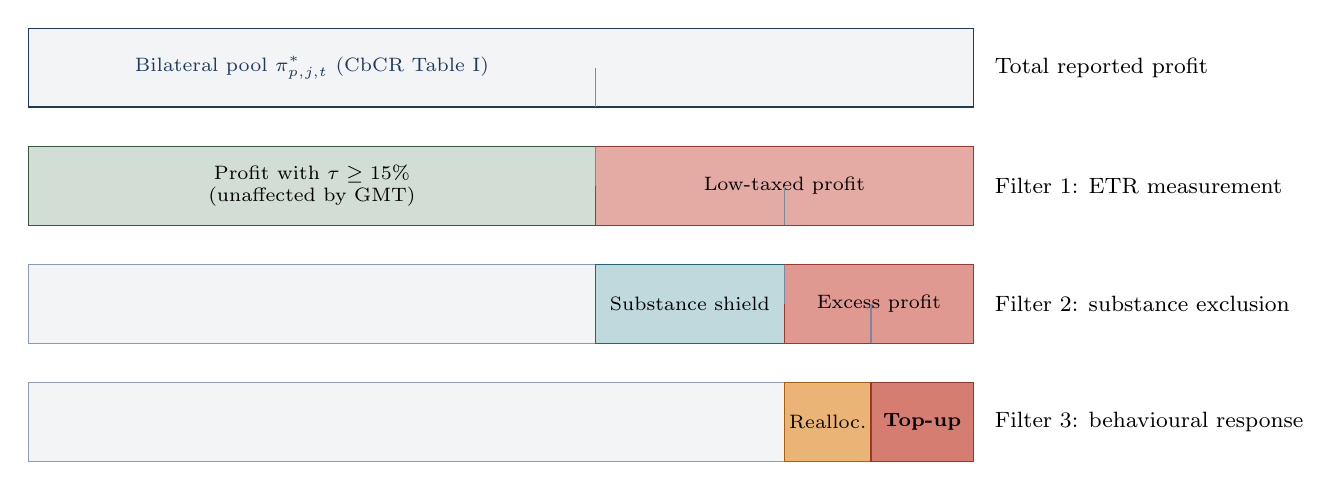
\begin{tikzpicture}[font=\small]
  % Total profit bar
  \def\tw{12}
  \def\th{1.0}

  % Layer 1: total profit
  \fill[thesisLight, draw=thesisNavy, line width=0.6pt] (0,4) rectangle (\tw, 4+\th);
  \node[font=\footnotesize, anchor=west] at (\tw+0.15, 4+\th/2) {Total reported profit};

  % Layer 2: split into above-15 (left) and below-15 (right)
  \fill[thesisGreen!25, draw=thesisGreen!70!black] (0,2.5) rectangle (7.2, 2.5+\th);
  \fill[thesisRed!45, draw=thesisRed!80!black] (7.2,2.5) rectangle (\tw, 2.5+\th);
  \node[font=\scriptsize, align=center] at (3.6, 2.5+\th/2) {Profit with $\tau \geq 15\%$\\(unaffected by GMT)};
  \node[font=\scriptsize, align=center] at (9.6, 2.5+\th/2) {Low-taxed profit};
  \node[font=\footnotesize, anchor=west] at (\tw+0.15, 2.5+\th/2) {Filter 1: ETR measurement};

  % Layer 3: SBIE shield on the low-taxed portion
  \fill[thesisLight, draw=thesisNavy!50] (0,1.0) rectangle (7.2, 1.0+\th);
  \fill[thesisTeal!30, draw=thesisTeal!80!black] (7.2,1.0) rectangle (9.6, 1.0+\th);
  \fill[thesisRed!55, draw=thesisRed!80!black] (9.6,1.0) rectangle (\tw, 1.0+\th);
  \node[font=\scriptsize] at (8.4, 1.0+\th/2) {Substance shield};
  \node[font=\scriptsize, align=center] at (10.8, 1.0+\th/2) {Excess profit};
  \node[font=\footnotesize, anchor=west] at (\tw+0.15, 1.0+\th/2) {Filter 2: substance exclusion};

  % Layer 4: behavioural response carves into the excess profit
  \fill[thesisLight, draw=thesisNavy!50] (0,-0.5) rectangle (9.6, -0.5+\th);
  \fill[thesisOrange!55, draw=thesisOrange!80!black] (9.6,-0.5) rectangle (10.7, -0.5+\th);
  \fill[thesisRed!70, draw=thesisRed!80!black] (10.7,-0.5) rectangle (\tw, -0.5+\th);
  \node[font=\scriptsize, align=center] at (10.15, -0.5+\th/2) {\rotatebox{0}{Realloc.}};
  \node[font=\scriptsize, align=center] at (11.35, -0.5+\th/2) {\textbf{Top-up}};
  \node[font=\footnotesize, anchor=west] at (\tw+0.15, -0.5+\th/2) {Filter 3: behavioural response};

  % Connecting brackets
  \draw[thesisNavy!60, line width=0.4pt] (7.2, 4) -- (7.2, 3.5+\th);
  \draw[thesisNavy!60, line width=0.4pt] (7.2, 2.5+\th) -- (7.2, 2.0+\th);
  \draw[thesisNavy!60, line width=0.4pt] (9.6, 2.5) -- (9.6, 2.0+\th);
  \draw[thesisNavy!60, line width=0.4pt] (9.6, 1.0+\th) -- (9.6, 0.5+\th);
  \draw[thesisNavy!60, line width=0.4pt] (10.7, 1.0) -- (10.7, 0.5+\th);

  % Annotations
  \node[font=\scriptsize, thesisNavy] at (3.6, 4+\th/2) {Bilateral pool $\pi^{*}_{p,j,t}$ (CbCR Table I)};
\end{tikzpicture}
}
\caption[GMT revenue as successive filters on the multinational profit pool.]{GMT revenue as successive filters on the bilateral CbCR profit pool. Reading from top to bottom, the figure starts with total reported profit, isolates the profit taxed below 15\%, removes the substance-protected share, subtracts the behavioural reallocation response, and leaves the residual top-up tax base. These filters correspond to the measurement, substance and behavioural factors in the variance decomposition in Section \ref{sec:decomposition}.}
\label{fig:gmt_mechanics_intro}
\end{figure}

This paper addresses the following research question:

\begin{quote}
\textit{How much of the uncertainty in EU Global Minimum Tax revenue estimates from public 2017--2022 OECD CbCR data is generated by low-taxed-base measurement, substance exclusions, behavioural responses, and legal allocation rules?}
\end{quote}

Five subquestions break this into empirically tractable parts:
\begin{enumerate}[nosep,label=\textit{SQ\arabic*},leftmargin=2.5em]
  \item How much low-taxed profit is identified under jurisdiction-average, direct subsidiary-level and imputed distributional ETR measurement?
  \item How much do the substance exclusion and the substance-based tax incentive exposure reduce the effective tax floor across EU countries and sectors?
  \item What behavioural semi-elasticity is supported by the 2017--2022 CbCR panel, and how reliable is that estimate under fixed-effect, model-selection, IV and tail-support diagnostics?
  \item How do the source-country top-up, the parent-country backstop, the enforcement backstop and the Side-by-Side safe harbour redistribute or extinguish top-up tax across EU Member States?
  \item Do EU Member States separate into policy-relevant types once fiscal exposure, legal allocation risk and measurement uncertainty are observed jointly?
\end{enumerate}

Across the 32 scenarios, cumulative EU top-up tax revenue over 2017--2022 ranges from US\$128 billion to US\$517 billion. The decomposition reveals a clear ranking. ETR measurement explains 69.1\% of pooled scenario variance: moving from jurisdiction-average to distributional measurement nearly doubles the estimated revenue. The allocation regime explains 15.0\%: the Side-by-Side safe harbour reduces average cumulative EU revenue from US\$326 billion to US\$238 billion by removing US-parented groups from the parent-country and enforcement backstops while leaving source-country top-up taxes in place. The behavioural response explains 5.1\% as a main effect. In the preferred scenario, applying the estimated linear semi-elasticity of 1.50 reduces cumulative EU revenue by approximately US\$47 billion. The semi-elasticity itself exceeds the \citet{heckemeyer2017} consensus of 0.8 but is well below the steep low-rate response in \citet{dowd2017}. The Bayesian information criterion selects the linear Hines--Rice specification over logarithmic and quadratic alternatives. Interactions across all five factors account for 6.0\% of variance, confirming that the main effects dominate. The substance exclusion lowers the EU-wide profit-weighted effective floor from 14.2\% to 11.9\%, with the largest reductions in capital-intensive sector-country cells. A PCA-informed country typology separates EU Member States into four groups: high-salience conduit-exposed states, states protected by their own source-country top-up tax, states with residual parent-country backstop exposure, and states with negligible current exposure.

The paper contributes to the GMT revenue literature in five ways. First, it translates the public OECD CbCR data into a replicable measurement framework that shows the profits that are shifted and the decomposition within countries of shifted profit. Existing studies either use jurisdiction averages \citep{barake2022} or access confidential micro-data \citep{hugger2026}. This paper shows what public data can and cannot reveal about the low-taxed base. Second, it embeds the measured base in a full factorial design and decomposes the scenario spread through an orthogonal variance identity, attributing variation to five main effects and all interactions. Existing studies vary assumptions one at a time or decompose revenue for a single country \citep{boukal2026}. The factorial approach is the first to show that measurement and allocation dominate the spread jointly. Third, it provides a panel semi-elasticity estimate on the 2017--2022 CbCR data with bilateral parent-affiliate fixed effects, absorbing time-invariant confounders such as treaty networks and legal-system proximity that cross-sectional estimates cannot control for \citep{garcia-bernardo2024}. Three functional forms are estimated on the same sample and ranked by information criteria, producing directly comparable semi-elasticity schedules. Fourth, it constructs sector-specific effective tax floors for 27 EU Member States by combining CbCR data with Eurostat Foreign Affiliates Statistics and EU KLEMS capital-stock data, measuring how much the substance exclusion varies across sectors. Fifth, it adds an unsupervised country typology that compresses cross-country heterogeneity into policy-facing groups using PCA and clustering. The typology is a classification device for the revenue results. It does not make causal claims.

Section \ref{sec:litreview} reviews the profit-shifting literature, the Global Minimum Tax rules and the tax-competition mechanisms that motivate the hypotheses. Section \ref{sec:data} documents how the CbCR panel is constructed and cleaned and introduces the supplementary substance, sectoral, macro, tax-rate and legal-status data. Section \ref{sec:measurement_framework} turns those inputs into measured revenue objects. Section \ref{sec:methodology} estimates the behavioural semi-elasticity, maps it into a counterfactual reallocation factor, applies the allocation rules, defines the revenue equation, decomposes the 32-scenario spread and constructs the country typology. Section \ref{sec:results} reports the results in the same order: measured low-taxed profit, substance and SBTI exposure, behavioural estimates, allocation and factorial decomposition, country heterogeneity and hypothesis tests. Section \ref{sec:discussion} interprets the uncertainty ranking, policy implications and limitations. The appendices mirror this order. Appendix \ref{app:data} audits data construction, Appendices \ref{app:stage1_measurement}--\ref{app:stage4_allocation} document the four empirical stages, Appendix \ref{app:country_policy} collects country-level policy material, and the online replication material is separated from the reader appendix.

\section{Literature and institutional framework}\label{sec:literature}\label{sec:litreview}

Revenue uncertainty surrounding the Global Minimum Tax decomposes into four distinct channels: measurement of the low-taxed profit base, the behavioural semi-elasticity governing how MNEs reallocate profits in response to the new floor, substance-based exclusions that reduce the effective minimum rate below its headline 15\%, and the legal allocation rules that determine which government collects the top-up tax. Plausible alternatives within any single channel produce revenue estimates that differ by factors of two or more. Section \ref{sec:beps} establishes the profit-shifting magnitudes the GMT targets. Section \ref{sec:design} describes the legal mechanics. Section \ref{sec:theory_lit} connects tax-competition welfare models to the contested semi-elasticity values. Sections \ref{sec:measurement}--\ref{sec:allocation_lit} ground each uncertainty channel in institutional detail and empirical evidence, and Section \ref{sec:theoretical_framework} synthesises them into testable hypotheses.

\subsection{From profit shifting to GMT revenue uncertainty}\label{sec:beps}

The foundational approach to estimating profit shifting uses the Hines--Rice framework, which regresses pre-tax profit on local GDP, labour inputs and the statutory tax rate to recover a semi-elasticity of reported profits with respect to taxation \citep{hines1994}. \citet{heckemeyer2017} meta-regress 27 studies conducted in this tradition and find a consensus tax semi-elasticity of approximately 0.8. 

\citet{dowd2017} demonstrate this nonlinearity using US Internal Revenue Service (IRS) administrative data on Controlled Foreign Corporations (CFCs) covering the period 2002--2012. Their quadratic specification yields a semi-elasticity of approximately 4.7 at a 5\% statutory rate, compared to only 0.7 at 30\%. \citet{garcia-bernardo2024} formalise the insight with a logarithmic specification applied to Organisation for Economic Co-operation and Development (OECD) Country-by-Country Reporting (CbCR) data, estimating \$850 billion in shifted profits in 2017. Both estimates exceed the \$616 billion that \citet{torslov2023} report for 2015 using Foreign Affiliates Statistics (FATS), partly because the nonlinear specifications capture the concentration of shifting at very low rates. \citet{garcia-bernardo2022a} find that the share of US multinational enterprise (MNE) foreign profits booked in tax havens remained stable at approximately 50\% after the 2017 Tax Cuts and Jobs Act (TCJA), despite a 3--5 percentage point (pp) decline in the share booked abroad overall. This indirectly shows that the shifting incentive at very low effective tax rates (ETRs) survived a reform that narrowed the differential at moderate rates.

The magnitudes of profit shifting are contested. \citet{blouin2023} demonstrate that standard data sources suffer from systematic double counting through equity-method accounting and intermediate holding structures. When they replicate \citet{clausing2016} using corrected `Net Income Excluding Equity Income', the US revenue-loss estimate falls by approximately 90\%. Their reanalysis of \citet{torslov2023} suggests that removing equity income reduces the bilateral imputation by approximately half. The correction is directly relevant to the present study: CbCR-based revenue estimates inherit the same double-counting exposure, and this thesis applies a profit correction in Stage 1 (Section \ref{sec:doublecounting}) to address it.

\citet{garcia-bernardo2023} provide country-level ETR estimates for 47 countries using Orbis unconsolidated data for 2011--2015, finding that ETRs diverge substantially from statutory rates in several conduit jurisdictions (Luxembourg: 1--8\% ETR versus 29\% statutory). \citet{johansson2017} confirm that the largest MNEs reduce ETRs by 4--8.5 pp through profit shifting, with global corporate income tax (CIT) losses of 4--10\%. \citet{bilicka2026} exploit variation in German municipal business tax rates and find that subsidiaries of MNEs with haven affiliates respond more aggressively to local tax increases, consistent with the nonlinear pattern identified by \citet{dowd2017}.\footnote{\citet{cobham2018} show that lower-income countries lose a larger share of CIT revenue to profit shifting. \citet{riedel2018} provides a review that confirms the consensus semi-elasticity while emphasising identification challenges in developing-country settings.}


\subsection{Global Minimum Tax mechanics}\label{sec:design}

The Global Minimum Tax imposes a minimum effective tax rate of 15\% on the GloBE income of MNE groups with consolidated revenue above EUR 750 million \citep{oecd2025}. The top-up tax equals the difference between 15\% and the jurisdictional ETR, applied to the excess profit base, defined as GloBE income minus the Substance-Based Income Exclusion (SBIE). \citet{barake2022} provide the first systematic estimate of GMT revenue: approximately EUR 179 billion globally under an Income Inclusion Rule (IIR)-first scenario, assuming no behavioural response. They acknowledge a binding limitation: their calculation applies jurisdiction-average ETRs, treating all profit within a jurisdiction as either entirely above or entirely below the 15\% threshold.

Three collection mechanisms operate in a strict waterfall. The Qualified Domestic Minimum Top-Up Tax (QDMTT) gives the source jurisdiction first collection rights. If no QDMTT exists, the IIR allows the parent jurisdiction to collect. The Undertaxed Profits Rule (UTPR) serves as the backstop, allocating residual liability to jurisdictions where the MNE has tangible assets and employees. \citet{devereux2022} show that the QDMTT priority effectively reverses the original IIR-first logic, creating a `QDMTT race' in which source jurisdictions pre-emptively raise their tax floor to retain revenue domestically. The result is a Nash equilibrium in which adoption is a dominant strategy: every jurisdiction that expects to host low-taxed MNE affiliates enacts a QDMTT regardless of what other jurisdictions do.\footnote{\citet{hanlon2023} notes that GloBE income diverges from CbCR financial profit through timing differences, loss carryforwards and permanent differences, creating a wedge between CbCR-based ETRs and the actual GloBE ETR. This wedge introduces measurement noise that all CbCR-based revenue estimates, including the present study, must acknowledge.}

The January 2026 Side-by-Side (SbS) Safe Harbour disrupts this waterfall \citep{oecd2026}. MNE groups headquartered in jurisdictions with a `Qualified SbS Regime' may elect a deemed top-up of zero under both IIR and UTPR, leaving QDMTTs as the only operative top-up channel for those groups. The pipeline source used in this paper lists the United States as the qualified SbS jurisdiction \citep{oecdCentralRecord2026}. The SbS creates a sharp discontinuity in collection rights without altering the underlying volume of low-taxed profit. For EU Member States that have enacted a QDMTT, collection against US-owned affiliates is unaffected. For those that have not, the residual IIR and UTPR claim disappears entirely. This asymmetry makes the allocation rule a first-order source of cross-country revenue heterogeneity.

\subsection{Tax competition and welfare under minimum taxation}\label{sec:theory_lit}

The welfare effect of a minimum tax is theoretically ambiguous. \citet{johannesen2022} models a large non-haven and a small haven competing for mobile profits. A minimum tax raises non-haven welfare when it eliminates more profit shifting than the associated compliance and distortion costs destroy. The net effect depends on two parameters: the semi-elasticity of profit shifting and the government's relative weight on firm-owner consumption versus public goods. At the \citet{heckemeyer2017} consensus semi-elasticity of 0.8, the welfare effect is negative: the minimum tax reduces shifting too little to compensate for the distortion it introduces. At the \citet{dowd2017} quadratic values exceeding 1.8 at low ETRs, the effect turns positive. This threshold dependence explains why the semi-elasticity channel matters for economic policy planning: the same institutional reform is welfare-enhancing or welfare-reducing depending on a coefficient that the literature has not pinned down.

\citet{hebous2023} identify conditions under which a minimum tax can be Pareto-improving: all countries can be made better off if appropriate lump-sum transfers accompany the minimum. The result requires that the minimum rate stay below the cooperative optimum, a condition that is empirically testable and depends on the same contested semi-elasticity. \citet{vantriet2025} provide the first quantitative welfare assessment, simulating the GMT in the CORTAX computable general equilibrium model for the EU-27, the United States, the United Kingdom, Japan and a stylised tax haven. The welfare-optimal minimum rate is 16\% (1 pp higher than the enacted 15\% GMT) and the simulation satisfies the Hicks--Kaldor compensation test: aggregate gains exceed aggregate losses, so winners could in principle compensate losers. Crucially, their robustness analysis varies the semi-elasticity from 0.54 to 1.03 (the \citet{heckemeyer2017} 95\% confidence interval) and the optimal rate is robust while the welfare-gain magnitude changes substantially, confirming that coefficient uncertainty translates to policy conclusions.

\citet{janeba2023} model the strategic interaction after GMT implementation. The GMT eliminates the incentive for havens to set statutory rates below 15\%, but simultaneously increases the incentive for non-havens to compete for real economic activity through subsidies, infrastructure provision and regulatory concessions. When competition uses lump-sum instruments, the revenue gains from reduced profit shifting are exactly offset by increased subsidy expenditure. The practical implication is that Pillar Two shifts tax competition from headline rates toward opaque instruments that the SBIE and the Substance-Based Tax Incentive (SBTI) Safe Harbour partially accommodate.

Two further theoretical results bear on the revenue estimate. \citet{schjelderup2024} show that the SBIE does more than reduce the top-up tax base. Because payroll costs and tangible assets are partly deductible again for Pillar Two purposes, the SBIE acts like an implicit production subsidy for affiliates in low-tax jurisdictions with real activity. In their calibration, the effective rental cost of capital falls by 0.50--0.96\% (for machinery and buildings), while the wage-cost reduction is bounded at 0.88\%. The mechanism therefore tends to favour capital-intensive affiliates, partly offsets the reduction in transfer-pricing incentives, and creates a remaining margin of real-activity competition under Pillar Two. \citet{jean2026} introduce an enforcement dimension: the GMT may reduce the incentive for low-tax countries to cooperate on transfer-pricing enforcement, because the top-up tax is collected by the high-tax parent or QDMTT jurisdiction rather than by the source country that bears the enforcement cost. When the minimum rate exceeds a critical threshold, the low-tax country withdraws from enforcement cooperation entirely, potentially \textit{increasing} profit shifting in the long run. The implication for revenue estimates is that assuming a fixed semi-elasticity may overstate the GMT's behavioural effect in jurisdictions that respond by reducing enforcement effort.

\subsection{Measuring the low-taxed base}\label{sec:measurement}

\citet{hugger2026} provide the central empirical fact for this channel: 53.2\% of all globally low-taxed profit (below a 15\% ETR) lies in jurisdictions where the \textit{average} ETR exceeds 15\%. The within-jurisdiction dispersion in ETRs (driven by firm-level variation in loss histories, incentive claims and financing structures) is often larger than the cross-jurisdiction dispersion. This finding implies that jurisdiction-level analyses substantially underestimate the volume of low-taxed profit and correspondingly the revenue from the GMT. Their estimates place annual low-taxed profit of large MNEs at USD 2,143 billion, with more than half located outside the traditional investment hubs that dominate BEPS discussions.

Earlier revenue estimates do not incorporate this within-jurisdiction heterogeneity. \citet{barake2022} apply jurisdiction-average ETRs, explicitly acknowledging that this approach understates the GMT base. The bias is large: their estimate of EUR 179 billion assumes that all profit within a jurisdiction faces the jurisdiction-average ETR, so that a jurisdiction with an average ETR above 15\% contributes zero low-taxed profit, regardless of the within-jurisdiction distribution. The discrepancy between average and distributional measurement is the single largest source of revenue disagreement identified in the literature reviewed here.

The reliability of CbCR-based ETRs is itself uncertain. \citet{bobeldijk2019} identify four definitional problems in CbCR data: ambiguous dividend treatment inflates profits without corresponding tax entries, the exclusion of deferred taxes depresses measured ETRs, loss carryforwards create false-positive zero-ETR entries for jurisdictions that are not genuinely low-taxed, and within-country aggregation double-counts intra-country intercompany transactions. \citet{godar2024} find that ETRs computed from voluntarily published CbCRs average 25\%, far above the 14\% implied by aggregate OECD CbCR data, suggesting that the aggregate data overstates the low-taxed share for transparent MNEs and that selection into public reporting is non-random. \citet{blouin2023} show that the double-counting problem inflates the ETR denominator, mechanically depressing measured rates and inflating top-up estimates. 

\subsection{Behavioural responses: semi-elasticity level and functional form}\label{sec:behaviour}

Three functional forms dominate the literature, and they disagree most at the ETRs where the GMT base is concentrated. \citet{heckemeyer2017} impose a constant semi-elasticity of 0.8: a one-percentage-point increase in the tax rate reduces reported profit by 0.8\%, irrespective of the initial rate. \citet{dowd2017} fit a quadratic that rises to 4.7 at a 5\% rate, implying that shifting is five times more responsive in the low-tax tail than at moderate rates. \citet{garcia-bernardo2024} fit a logarithmic specification that diverges as the rate approaches zero, producing even larger predicted responses at the bottom of the distribution. The GMT base concentrates in the 0--15\% ETR range \citep[\textit{cf.}][]{hugger2026}, precisely where the three specifications diverge most. Committing to any single functional form before estimation is therefore a prejudgement of the revenue answer.

Identification strategies vary across the three studies and each carries limitations. \citet{dowd2017} estimate on a US-only CFC panel with no cross-country variation in the parent-jurisdiction tax system, raising questions about external validity to European MNEs. \citet{garcia-bernardo2024} estimate on a single 2017 CbCR cross-section that cannot control for time-invariant bilateral confounders such as historical investment ties, treaty networks and language proximity. \citet{heckemeyer2017} synthesise 27 studies with heterogeneous methodologies, and their confidence interval (0.54 to 1.03) spans a range over which the welfare conclusions of \citet{johannesen2022} and the revenue predictions of \citet{vantriet2025} change sign. None of the three studies estimates the behavioural response conditional on the GloBE regime, all extrapolate from pre-GMT tax variation.

The CbCR panel population may itself be a treatment group. \citet{tuinsma2025} exploit the EUR 750 million CbCR filing threshold in a regression discontinuity design and find that private CbCR reporting raised ETRs by approximately 6 pp for moderately aggressive MNEs. The most aggressive MNEs (those with established tax-haven structures) showed only a modest response, consistent with real substance that is costly to relocate. This heterogeneity implies that the semi-elasticity estimated from the CbCR population reflects a treated subpopulation whose tax behaviour was changing during the sample period, introducing a confound for any revenue estimate that applies the estimated coefficient to the full MNE population.

\subsection{Substance exclusions and the effective tax floor}\label{sec:substance_lit}

The statutory 15\% rate should not be read as a simple 15\% tax floor on all profit. Under the GMT, part of a company’s income is carved out before the top-up tax is calculated. This carve-out, the Substance-Based Income Exclusion (SBIE), is based on a fixed percentage of eligible payroll costs and tangible assets. As a result, firms with substantial employees or physical assets in a low-tax jurisdiction may face an effective tax floor below 15\% on their total profit. \citet{devereux2023} measure the SBIE-to-profit ratio using Amadeus data on foreign-owned EU subsidiaries and find an average of 57\% (52\% median) during the initial transition period, declining to 41\% (28\% median) at long-run rates (ten years). The effective minimum tax on GloBE income is therefore approximately 6.45\% in the first year, rising to 8.85\% after the transition completes. Approximately 30\% of subsidiaries have SBIE exceeding pre-tax profit, facing zero top-up tax regardless of their ETR. These magnitudes make the SBIE a structural feature that halves the effective tax floor for the median subsidiary, rather than a marginal adjustment.

The SBIE creates a new competitive margin. \citet{schjelderup2024} show within a two-country model that the SBIE functions as a \textit{de facto} production subsidy, lowering the effective cost of capital for real investment in low-tax jurisdictions. The reduction in the rental cost of capital (0.50--0.96\%) exceeds the reduction in the effective wage rate (up to 0.88\%), meaning that the SBIE favours capital-intensive industries and generates sector-specific distortions. \citet{janeba2023} predict that tax competition after GMT implementation shifts from headline rates toward subsidies and regulatory instruments. The SBIE provides the formal channel through which this competition operates. Jurisdictions with large tangible-asset bases (for instance, manufacturing hubs in Central and Eastern Europe) benefit disproportionately, while service-oriented economies with thin fixed-asset bases gain little SBIE protection.

The January 2026 SBTI Safe Harbour introduces a second substance channel \citep{oecd2026}. Qualifying tax incentives (QTIs) may be treated as additions to covered taxes rather than reductions, inflating the ETR numerator and preventing artificial ETR depression. The benefit is bounded by a Substance Cap tied to the larger of payroll costs and the carrying value of tangible assets. \citet{ferreiraliotti2022} document that the impact of tax incentives under Pillar Two varies dramatically by type: accelerated depreciation has low impact because it creates timing differences rather than permanent level effects, while tax holidays and intellectual-property (IP) box regimes have high impact because they reduce the ETR below 15\% on a permanent basis. The SBTI explicitly protects expenditure-based incentives up to the Substance Cap, carving out incentives that reward genuine economic activity while leaving pure profit-shifting vehicles exposed. 

\subsection{Legal allocation: who collects the top-up tax}\label{sec:allocation_lit}

The same euro of low-taxed profit can flow to different governments depending on the allocation rule. Under the standard GloBE waterfall, the source jurisdiction collects via a QDMTT. Absent that, the parent jurisdiction collects via the IIR. Absent that, third countries collect via the UTPR in proportion to their shares of the MNE's tangible assets and employees. \citet{barake2022} estimate revenue under an IIR-first scenario, acknowledging that QDMTT adoption shifts revenue from parent to source jurisdictions. Drawing on \citet{devereux2022}, the QDMTT creates a Nash equilibrium in which every source jurisdiction pre-emptively raises its floor to 15\% to retain revenue domestically, effectively reversing the original IIR-first design logic. The allocation rule thus determines both the cross-country distribution of a given aggregate liability and, through strategic responses, the aggregate itself.

The January 2026 SbS Safe Harbour introduces a discontinuity. US-parented MNE groups may elect a deemed top-up of zero under both IIR and UTPR \citep{oecd2026}. QDMTTs remain unaffected: EU Member States that have enacted a QDMTT retain their collection right against US-owned low-taxed affiliates, while those that have not lose the residual claim entirely. The Dutch Ministry of Finance revised its annual GMT revenue projection downward by EUR 122 million following the SbS package \citep{1028}. For the EU as a whole, the SbS leaves the aggregate volume of US-parented low-taxed profit in place and concentrates the collection right among the subset of Member States with an operative QDMTT, creating a wedge between the `universal' and `SbS' allocation regimes.

\citet{boukal2026} decompose GMT revenue for Slovakia and show that the composition varies dramatically across collection channels: QDMTT, IIR and behavioural responses each contribute different shares depending on the modelling assumptions applied. Their single-country analysis demonstrates that allocation interacts with the measurement and behavioural channels. \citet{cobham2022} propose an alternative allocation mechanism: the Minimum Effective Tax Rate (METR), which would replace the QDMTT/IIR/UTPR waterfall with formulary apportionment keyed to sales, employment and assets. The factorial design developed in this thesis makes the allocation channel directly comparable with measurement and behavioural channels in variance-explained terms.

\subsection{Synthesis and hypotheses}\label{sec:theoretical_framework}\label{sec:hypotheses}

The preceding four subsections establish the four sources of GMT revenue uncertainty: how the low-taxed profit base is measured, how MNEs respond behaviourally to the new floor, how the Substance-Based Income Exclusion carves out part of the base, and which government ultimately collects the top-up tax. Each source corresponds to at least one contested modelling choice. This section translates those choices into a structured empirical design and derives five testable predictions.

The core empirical strategy is a $2^5$ factorial simulation. Five binary factors are crossed: (F1) how the low-taxed profit base is measured (jurisdiction-average ETR versus distributional ETR), (F2) how substance exclusions are specified (aggregate versus sectoral), (F3) which SBIE carve-out rates apply (initial transition rates versus long-run steady-state rates), (F4) which allocation rule governs collection rights (the standard GloBE waterfall versus the January 2026 Side-by-Side Safe Harbour regime), and (F5) which semi-elasticity governs the behavioural response (constant versus nonlinear specification). The 32 resulting scenarios each represent a specific combination of policy and modelling choices. Comparing these scenarios is the methodological contribution of this paper. Unlike prior work that varies one assumption at a time \citep{barake2022,hugger2026} or decomposes revenue for a single country \citep{boukal2026}, this design allows all five channels to vary simultaneously while keeping their contributions separable.

\subsubsection*{H1: Distributional ETR measurement produces a larger low-taxed profit base than jurisdiction-average measurement.}

\citet{hugger2026} show that 53.2\% of globally low-taxed profit sits in jurisdictions where the \emph{average} ETR exceeds 15\%. The jurisdiction-average approach, which is standard in the revenue estimation literature \citep{barake2022}, assigns zero low-taxed profit to such jurisdictions and therefore misses more than half of the true base. By contrast, the distributional measurement branch used in this paper draws on Table~IV ETR brackets to recover the within-jurisdiction spread of profit across ETR intervals, capturing the firm-level mass that the average conceals.

The direction of the prediction is unambiguous: switching from jurisdiction-average to distributional measurement must weakly increase the measured low-taxed base. The null hypothesis is that the two approaches produce the same low-taxed liability. The magnitude of the difference depends on how well the within-jurisdiction distributional approximation tracks the true firm-level distribution, which only confidential microdata could fully resolve. The formal null is: the low-taxed liability is the same under distributional and jurisdiction-average ETR measurement.

\subsubsection*{H2: The ETR measurement method explains the largest share of revenue variance across the 32 scenarios.}

Even if each of the five binary factors shifts the revenue estimate, they need not contribute equally to the spread of outcomes. The variance decomposition answers which factor matters most for the uncertainty that policymakers face.

The measurement factor (F1) operates at the very first stage of the revenue pipeline: it determines the volume of profit on which the top-up rate, the SBIE reduction, the behavioural correction and the allocation weight subsequently act. Because all four later stages are multiplicative on the base, a large base-level shift propagates through every subsequent calculation. The SBIE, behavioural and allocation factors each apply to a progressively smaller residual and therefore have a structurally bounded scope to drive variance. If the Hugger finding, that more than half of the low-taxed base is invisible to the jurisdiction-average rule, holds in the EU-27 sample, the base-level shift from F1 should dominate the variance decomposition. The null hypothesis is that the five main effects explain equal shares of variance ($\eta_1^2 = \eta_k^2$ for all $k$). Rejecting this null in favour of F1 dominance has a direct policy implication: improving the quality of ETR measurement data yields larger reductions in revenue uncertainty than resolving debates about the semi-elasticity or the SBIE specification.

\subsubsection*{H3: The Side-by-Side Safe Harbour is the second-largest source of scenario variance and materially redistributes GMT revenue across EU Member States.}

The January 2026 SbS Safe Harbour does not change the volume of low-taxed profit. It changes who collects the corresponding top-up tax. For MNE groups headquartered in a qualifying SbS jurisdiction (currently only the U.S.) both the IIR and the UTPR collection rights are deemed zero, leaving the QDMTT as the only operative collection channel. EU Member States that have enacted a QDMTT retain their collection right against US-parented low-taxed affiliates unchanged. Member States without an operative QDMTT lose their residual IIR and UTPR claim entirely. Given that US-parented MNEs hold the largest single share of foreign direct investment in the EU \citep[\textit{cf.}][]{oecd2025}, this asymmetry translates into a material reallocation of collection rights across Member States. The Dutch Ministry of Finance quantified part of this effect, revising its annual GMT revenue projection downward by EUR~122~million following the SbS package \citep{1028}.

The prediction is that the SbS allocation factor (F4) ranks second in the variance decomposition after the measurement factor (F1). The SbS operates on a large share of EU affiliate profit and concentrates its impact on countries with specific legal characteristics (QDMTT adoption), creating substantial cross-country heterogeneity. The null hypothesis is that the SbS factor does not change aggregate EU-27 GMT revenue, does not rank among the two largest variance sources, and does not alter the cross-country distribution of revenue across collection channels.

\subsubsection*{H4: The CbCR panel supports a negative tax--profit relationship, but does not require a nonlinear specification.}

A higher effective tax rate in a jurisdiction should reduce the pre-tax profit that MNEs report there. This is the fundamental prediction of the Hines--Rice framework and the profit-shifting literature \citep{heckemeyer2017,dowd2017,garcia-bernardo2024}: when shifting is cheaper than paying local tax, MNEs move reported profit toward low-tax affiliates. The contested question is not whether this relationship exists, but whether it is approximately linear or sharply nonlinear at very low ETRs. \citet{dowd2017} find that the semi-elasticity rises to 4.7 at a 5\% ETR, which is six times the linear consensus estimate of \citet{heckemeyer2017}, implying much larger predicted profit reallocation under the GMT for firms currently at very low ETRs.

This nonlinearity may not survive estimation on the public CbCR panel. The CbCR data are aggregated to jurisdiction--year cells, averaging across all firms within each cell and smoothing away the within-cell heterogeneity that drives the nonlinear lower tail in firm-level data \citep{dowd2017}. Furthermore, \citet{tuinsma2025} show that the CbCR reporting population is itself a treated group: mandatory reporting raised ETRs during the sample period, compressing the low-ETR variation needed to identify curvature. The prediction is therefore that the data support a significant negative tax--profit relationship, but that BIC-based model selection favours the constant-elasticity specification over the quadratic alternative. The null hypothesis is that tax terms are jointly insignificant or that model selection requires a nonlinear specification.

\subsubsection*{H5: EU Member States cluster into distinct policy profiles along three dimensions: fiscal salience, allocation exposure and measurement risk.}

The previous four hypotheses concern the aggregate revenue distribution. H5 concerns its cross-country structure. If each Member State's exposure to GMT revenue uncertainty is shaped by a different combination of the four channels, then countries may differ systematically along multiple dimensions simultaneously and that multidimensional structure may be recoverable through standard classification methods.

Three dimensions drive the prediction. Fiscal salience varies because large economies with broad domestic CIT bases are less sensitive to GMT revenue changes than small open economies that host MNE headquarters or intermediate holding structures. Allocation exposure varies because the SbS factor differentially affects countries depending on their share of US-parented affiliates and whether they have enacted a QDMTT. Measurement risk varies because the gap between distributional and jurisdiction-average ETR measurement depends on the within-country dispersion of firm-level ETRs, which \citet{hugger2026} show is jurisdiction-specific. These three dimensions are conceptually orthogonal: a country can have high fiscal salience but low allocation exposure (large QDMTT-equipped source country), or low salience but high allocation exposure (small non-QDMTT jurisdiction with US-heavy affiliate population). Standard clustering applied to the scenario-spread profiles across these dimensions should therefore produce interpretable country groupings. The null hypothesis is that country-level exposure is not systematically separable into distinct clusters. Rejecting it enables targeted policy recommendations: countries should improve measurement data, enacting a QDMTT, or managing semi-elasticity uncertainty rather than requiring bespoke country-by-country analysis.

\section{Data}\label{data}\label{sec:data}\label{sec:descriptive}

\subsection{OECD Country-by-Country Reporting}\label{sec:CbCR}

The primary source is the OECD public Country-by-Country Reporting (CbCR) database \citep{oecd2025a}. The data are based on anonymised and aggregated reports submitted to tax administrations by multinational groups above the \EUR 750 million consolidated-revenue threshold. This threshold makes CbCR close to the population targeted by Pillar Two. However, CbCR reports accounting aggregates rather than the adjusted covered taxes and GloBE income used in the GMT calculation \citep{oecd2025,hanlon2023}.

\subsubsection{Overview of CbCR data}\label{sec:CbCR_overview}

The main sample covers fiscal years 2017--2022. The analysis omits 2016 because CbCR filing was still transitional and less comparable across countries. Monetary variables remain in current US dollars. The OECD releases six CbCR tables. This thesis uses Table I and Table IV as the main inputs. Table I is the broad panel source: it reports profit before income tax, tax accrued, revenues, tangible assets, employees and activity counts by parent-affiliate-year cell. It also reports jurisdiction-average ETRs and, for later years, selected ETR percentiles. Table IV groups financial variables by ETR bracket. It shows how much pre-reform profit is located in lower and higher ETR parts of the public CbCR distribution. Tables II, III, V and VI provide robustness context, including robust means, group-level ETR brackets and size distributions. Appendix \ref{app:CbCR}, Table \ref{tab:cbcr_raw_architecture}, records the full table architecture.

Each observation links two jurisdictions in one fiscal year. The first is the parent jurisdiction ($p$), where the multinational group is headquartered. The second is the affiliate jurisdiction ($j$), where the group reports profit, tax, employees and tangible assets. Most of the measurement in this paper starts on the affiliate side, because that is where the low-taxed profit and substance variables are observed. The parent side is kept because it determines which country may collect residual top-up tax when the source country does not collect first. The empirical cell is therefore a parent-affiliate-year observation, denoted $(p,j,t)$.

The raw CbCR panel is cleaned into a bilateral panel. The full 2017--2022 analytical panel contains 15{,}758 parent-affiliate-year cells across 58 parent jurisdictions and 228 affiliate jurisdictions. This is the simulation frame. The EU27 affiliate slice is the source-country subset used for EU revenue results. The positive-profit sample contains 11{,}872 cells, or 75.3\% of the analytical panel, across 52 parents and 220 affiliates. This is the sample in which ETRs, low-taxed profit and top-up gaps can be measured. The behavioural estimation sample is narrower, containing 8{,}971 cells, or 56.9\% of the analytical panel, since the Hines--Rice regression is estimated in logs and therefore requires positive corrected profit, positive tangible assets and a positive wage-based payroll proxy. It also requires at least two observations for the same parent-affiliate pair so that the pair fixed effect is identified. Cells that lack one of these ingredients can still matter for the revenue simulation, but they cannot identify the semi-elasticity. Table \ref{tab:data_sample_construction} maps these empirical objects, while Appendix Section \ref{sec:base_panel_appendix} and Appendix Table \ref{tab:cleaned_panel_support} report the broader merged-panel coverage, support diagnostics and readiness flags that sit behind the sample restrictions.

% Generated by code/08_generate_results_tables.R
{\footnotesize
\setlength{\tabcolsep}{3pt}
\begin{longtable}{@{}L{3.6cm}rrrr>{\raggedright\arraybackslash}p{5.8cm}@{}}
\caption[Sample construction]{Sample construction and empirical objects}
\label{tab:data_sample_construction}\\
\toprule
Sample & Obs. & Parents & Affiliates & Share (\%) & Main use \\
\midrule
\endfirsthead
\multicolumn{6}{c}{\textit{Table~\ref{tab:data_sample_construction}---continued}} \\
\toprule
Sample & Obs. & Parents & Affiliates & Share (\%) & Main use \\
\midrule
\endhead
\midrule
\multicolumn{6}{r}{\textit{Continued on next page}}\\
\endfoot
\bottomrule
\endlastfoot
\multicolumn{6}{@{}l}{\textit{Panel A: source construction}} \\
Raw OECD Table I records & 1,124,211 & 58 & 240 &  & Raw source \\
Country parent-affiliate-year cells & 16,915 & 58 & 228 &  & Reshaped bilateral panel \\
2017--2022 analytical panel & 15,758 & 58 & 228 & 100.0 & Simulation frame \\
\addlinespace[0.2em]
\multicolumn{6}{@{}l}{\textit{Panel B: analysis samples}} \\
EU27 affiliate slice & 3,610 & 49 & 27 & 22.9 & EU source-country results \\
Positive-profit tax sample & 11,872 & 52 & 220 & 75.3 & ETRs and top-up gaps \\
Behavioural estimation sample & 8,971 & 47 & 151 & 56.9 & Hines--Rice semi-elasticity \\
\end{longtable}
}

\vspace{0.35em}
\noindent\begin{minipage}{\textwidth}
\footnotesize\raggedright\textit{Notes:} Share is relative to the 2017--2022 analytical panel.
\end{minipage}


\subsubsection{Correction for double-counted profit}\label{sec:doublecounting}

An effective tax rate (ETR) is a ratio: current-year income tax accrued \emph{divided} by profit. If profit is counted twice but tax is not, the measured ETR becomes too low even when the underlying tax position has not changed. Public CbCR profit data can suffer from this problem through intra-group dividends and ownership chains. Suppose a German ultimate parent owns a Dutch holding company, which in turn owns an Irish operating subsidiary. The Irish operating profit may be reported once as Irish affiliate profit and again as Dutch holding-company profit if the Dutch entity records dividend or participation income from the Irish subsidiary. \citet{blouin2023} show why this matters for profit-shifting estimates: the tax numerator is usually not inflated in the same way, so double-counted profit mechanically depresses ETRs. \citet{garcia-bernardo2022a} and \citet{hugger2026} correct the problem with richer reconciliation data. 

The CbCR data does not identify the underlying dividend flows directly. The correction is a bounded measurement adjustment for the domestic ultimate-parent correction share, denoted by $\rho_{pt}$. The model uses four observable signals: OECD adjusted-profit cells where available, official country-note evidence, the US macro reconciliation in \citet{garcia-bernardo2022a}, and a low-precision domestic-versus-foreign ETR parity diagnostic following the logic in \citet{hugger2026}. Appendix Section \ref{sec:profit_correction_reproducibility} gives the model and validation. The Beta fitting problem, BSPI algorithm, shape-stability test and Table I versus Table IV cross-validation are explained in Appendix \ref{app:measurement_framework} and Appendix Table \ref{tab:app_stage1_crossval}.

Let $\pi_{pjt}$ denote reported CbCR profit for parent jurisdiction $p$, affiliate jurisdiction $j$, and year $t$, and let $\pi^{adj}_{pjt}$ denote the OECD adjusted-profit field where it is reported. The preferred profit denominator is:
\begin{equation}\label{eq:profit_reconciliation_branch}
\pi^{*}_{pjt} =
\begin{cases}
\pi^{adj}_{pjt}, & \pi^{adj}_{pjt}\text{ observed},\\
(1-\widehat{\rho}_{pt})\pi_{pjt}, & p=j \text{ and } \pi^{adj}_{pjt}\text{ unobserved},\\
\pi_{pjt}, & p\neq j.
\end{cases}
\end{equation}

The correction is concentrated in domestic UPE cells, that is, cells where the parent and affiliate jurisdiction are the same ($p=j$). This is where dividend and participation-income double counting is most likely to enter the public CbCR profit measure. Foreign affiliate cells are left unchanged in the preferred branch because public aggregate CbCR does not reveal ownership-chain dividend flows with enough precision.

Table \ref{tab:profit_correction_effects} shows a denominator adjustment, not new tax payments. Over 2017 to 2022, the correction reduces positive-profit CbCR profit from US\$46.7 trillion to US\$34.8 trillion, a reduction of 25.4\%. Direct OECD adjusted-profit cells account for US\$0.24 trillion of the reduction, external-anchor domestic cells for US\$2.82 trillion, and model-shrunk domestic UPE cells for the remainder. Foreign affiliate cells still account for 34.1\% of reported positive-profit CbCR profit, but they account for 0.0\% of the correction because the preferred branch leaves them unchanged. The Share column therefore distributes the US\$11.87 trillion reduction, rather than reported profit. Because the correction reduces the profit denominator, it raises the profit-weighted raw ETR from 15.4\% to 20.6\% in the positive-profit sample, and from 16.4\% to 26.8\% in domestic UPE cells. 

% Generated by code/08_generate_results_tables.R
\begin{table}[H]
\centering
\scriptsize
\caption[Profit-base correction]{Correction from public CbCR profit to the reconciliation profit branch, 2017 to 2022}
\label{tab:profit_correction_effects}
\begin{tabularx}{\textwidth}{@{}>{\raggedright\arraybackslash}Xrrrrrr@{}}
\toprule
Profit category & Cells & Unadjusted & Corrected & Reduction & Reduction (\%) & Share (\%) \\
\midrule
\multicolumn{7}{@{}l}{\textit{Panel A: profit-base adjustment, USD billions}} \\
OECD adjusted-profit cells &     36 &    851.0 &    609.2 &    241.9 & 28.4 &   2.0 \\
Domestic ultimate-parent cells &    282 & 29,951.4 & 18,241.3 & 11,710.1 & 39.1 &  98.0 \\
Foreign affiliates unchanged & 15,440 & 15,908.8 & 15,908.8 &      0.0 &  0.0 &   0.0 \\
\midrule
Total reconciliation branch & 15,758 & 46,711.2 & 34,759.3 & 11,951.9 & 25.6 & 100.0 \\
\addlinespace[0.5em]
\multicolumn{7}{@{}l}{\textit{Panel B: diagnostic support for adjusted-profit correction}} \\
\multicolumn{6}{@{}l}{Statistic} & Value \\
\midrule
\multicolumn{6}{@{}l}{Observed adjusted-profit cells} & 36 \\
\multicolumn{6}{@{}l}{Parents with observed adjusted profit} & 2 \\
\multicolumn{6}{@{}l}{Affiliate observations with adjusted profit} & 36 \\
\multicolumn{6}{@{}l}{Median adjusted-to-unadjusted ratio} & 0.749 \\
\multicolumn{6}{@{}l}{Observed ratio range} & 0.516 to 1.000 \\
\bottomrule
\end{tabularx}

\vspace{0.5em}
\begin{minipage}{0.96\textwidth}
\footnotesize\raggedright \textit{Notes:} Panel A is restricted to positive-profit analytical cells and reports current USD billions. Unadjusted profit is public CbCR profit before the accounting correction; corrected profit is the reconciliation branch used in the reported revenue pipeline. Panel B uses only cells with observed OECD adjusted profit. The observed support is too sparse for a thesis-estimated imputation model, so no regression coefficient is used to construct the correction. Source files: data/processed/diagnostics/step2\_profit\_correction\_by\_year.csv; data/processed/diagnostics/cbcr\_t1\_profit\_adj\_support\_by\_year.csv; data/processed/base\_panel.rds.
\end{minipage}
\end{table}



ETRs are computed only for cells with positive corrected profit. The ETR variable divides current-year income tax accrued by corrected pre-tax profit, because tax accrued is the closest analogue to covered taxes \citep{hanlon2023}. Because CbCR tax accruals can be negative, delayed or affected by one-off items, a bounded ETR construction is applied before measuring low-taxed profit. Small negative accrual noise is set to zero, large negative observations are excluded from the ETR measurement, and implausibly high ratios are capped. The exact thresholds, flag counts and sensitivity diagnostics are reported in Appendix \ref{app:measurement_framework}.

\subsubsection{Within-jurisdiction heterogeneity}\label{sec:within-jurisdiction}

Estimating GMT revenue requires knowing how much profit in each jurisdiction is taxed below the 15\% threshold. Jurisdiction averages are insufficient. As \citet{hugger2026} show, more than half of globally low-taxed profit sits in jurisdictions whose \emph{average} ETR exceeds 15\%. Public CbCR contains partial information on that within-jurisdiction distribution, but not in one complete table. Table IV directly reports subsidiary-level ETR brackets from 2019 onwards. Table I reports selected ETR percentiles only in the later vintages. The pre-2019 bilateral panel has no direct within-jurisdiction distributional support. This is a data limitation, not yet a revenue calculation. Section \ref{sec:etr_measurement} defines how these incomplete sources are selected and translated into Stage 1 low-taxed shares, while Appendix \ref{app:measurement_framework} documents the percentile fit, BSPI backcast and validation tests.

\subsection{Substance and sectoral data}\label{sec:sectoral_data}\label{sec:substance_data}

The Global Minimum Tax first identifies low-taxed profit, but it does not apply the top-up tax to that full amount. The Substance-Based Income Exclusion (SBIE) removes a fixed return on local payroll and tangible assets from the low-taxed base. Sectors differ in how much labour and capital they use. A sector with many employees or tangible assets receives a larger substance shield.

CbCR reports tangible assets and employees by host country, but it does not report payroll. Payroll is therefore reconstructed by multiplying the number of employees in each affiliate-year cell by a country-year wage benchmark. The wage hierarchy uses additional \emph{OECD average annual wage} data where available, \emph{ILO earnings} data where OECD coverage is missing, and the nearest available year for the same jurisdiction when no contemporaneous wage observation exists (only 3.9\% of the cases).

The sectoral bridge addresses a separate data problem. CbCR observes profit, tax, employees and tangible assets by host country, but not by sector. Eurostat \emph{inward FATS} and \emph{EUKLEMS \& INTANProd} observe activity by NACE sector for foreign-controlled enterprises in EU Member States, but they do not report corporate tax liabilities. No dataset therefore observes both the tax base and the sectoral structure of the activities that generate it. The sectoral bridge is used only to allocate country-level CbCR aggregates across sectors. This reconciliation follows the logic of macro profit-shifting work that combines FATS information with national accounts data \citep{torslov2023}.

The allocation uses the most direct sectoral variable available for each component of the model. Payroll is allocated with FATS personnel costs where possible, with employment-scaled and turnover-scaled shares as fallbacks when personnel costs are suppressed. Tangible assets are allocated with EUKLEMS tangible capital stock. Where capital-stock coverage is incomplete, FATS investment is used as a fallback. The profit denominator is allocated with FATS gross operating surplus, with value added and turnover as fallbacks. These shares distribute the CbCR country aggregates across EU host-country sectors for the SBIE and SBTI exposure analysis.

The bridge is restricted to the EU27 and uses the post-2021 FATS structure. This restriction is necessary because the FATS series changes around 2021: the pre-2021 data use a broader activity aggregate that is not directly comparable with the later NACE-based classification. In the 2022 reference matrix, the bridge contains 40 non-overlapping leaf sectors for each EU Member State, or 1{,}080 country-sector cells. Across these cells, 98.1\% of payroll is allocated directly from FATS personnel costs, 83.2\% of tangible assets from EUKLEMS capital-stock information including gap-filled cells, and 88.2\% of the profit denominator from FATS gross operating surplus. \emph{BEA} data on U.S.-parented affiliates are used only as an external validation benchmark and do not enter the baseline bridge. Appendix \ref{app:sector} reports the full allocation hierarchy, fallback rules, gap-filling procedure and bridge-quality diagnostics.

\subsection{Supplementary data}\label{sec:supplementary}

Several supplementary sources complete the panel. \emph{OECD statutory corporate income tax rates} benchmark CbCR ETRs and supply a lagged statutory-rate instrument in robustness checks. \emph{OECD forward-looking effective tax rates} supply the simulated fixed-project EATR instrument used in the behavioural diagnostics. \emph{World Bank GDP per capita} and population enter as affiliate-market controls. \emph{OECD BEPS implementation indicators} record CFC rules, interest limitation rules, hybrid mismatch rules, IP regimes, mandatory disclosure rules and CbCR requirements. Pillar Two legal status is taken from the \emph{OECD Central Record version for purposes of the GMT}. The data record source-country first collection through QDMTTs, parent-country collection through IIRs, residual enforcement through UTPRs and Side-by-Side safe-harbour status. The legal ordering of those rules is specified in Section \ref{sec:methodology}.

Appendix \ref{app:source_provenance} records the scripted source endpoints. Appendix \ref{app:data}, Table \ref{tab:data_sources_units}, records the original unit of each source and its role in the panel, and Appendix Section \ref{sec:base_panel_appendix} reports the merged-panel diagnostics used to separate data construction from the later revenue stages.

\subsection{Descriptive statistics and sample diagnostics}\label{sec:data_diagnostics}

Table \ref{tab:data_panel_coverage} gives the first descriptive overview. Coverage improves over time: analytical pair-years rise from 2{,}045 in 2017 to 2{,}777 in 2022, while parent coverage rises from 38 to 54 jurisdictions. The profit base also moves with the macro cycle. Corrected positive profit falls from US\$5.9 trillion in 2019 to US\$4.9 trillion in 2020, then rises to US\$7.1 trillion in 2021. The table includes the preferred low-taxed-profit diagnostic because it is the measured base to which later filters are applied. In the pooled panel, corrected positive profit is US\$34.8 trillion and preferred low-taxed profit is US\$15.6 trillion, or 44.8\%.

% Generated by code/13_generate_exhibits.R
\begin{table}[H]
\centering
\footnotesize
\setlength{\tabcolsep}{3pt}
\caption[Analytical panel coverage by fiscal year]{Analytical panel coverage by fiscal year}
\label{tab:data_panel_coverage}
\begin{tabular}{@{}lrrrrrrrr@{}}
\toprule
Year & Pair-years & Parents & Affiliates & Positive pairs & EU27 pairs & Profit (US\$ bn) & Low-taxed profit (US\$ bn) & Median ETR \\
\midrule
2017 & 2,045 & 38 & 217 & 1,554 & 444 & 4,563.2 & 2,118.5 & 14.7 \\
2018 & 2,554 & 46 & 214 & 1,932 & 572 & 5,370.1 & 2,427.7 & 15.0 \\
2019 & 2,711 & 50 & 211 & 2,026 & 626 & 5,913.6 & 2,653.0 & 14.8 \\
2020 & 2,750 & 52 & 213 & 2,011 & 645 & 4,896.3 & 2,111.0 & 14.9 \\
2021 & 2,922 & 52 & 212 & 2,259 & 677 & 7,090.0 & 3,520.4 & 15.0 \\
2022 & 2,786 & 54 & 209 & 2,090 & 653 & 7,001.7 & 2,762.7 & 15.0 \\
2023 & 3,186 & 58 & 227 & 2,236 & 713 & 7,074.0 & 2,627.3 & 15.1 \\
Pooled & 18,954 & 63 & 232 & 14,108 & 4,330 & 41,909.0 & 18,220.6 & 15.0 \\
\bottomrule
\end{tabular}

\vspace{0.35em}
\noindent\begin{minipage}{\textwidth}
\footnotesize\raggedright\textit{Notes:} 2017--2023 Stage 1 panel; profit in USD bn; median ETR among positive-profit cells.
\end{minipage}
\end{table}


Table \ref{tab:data_summary_statistics} presents the summary statistics. The panel is highly skewed. The mean corrected-profit cell is US\$2.9 billion, the median is US\$77.1 million and the 90th percentile is US\$2.7 billion. A small number of large cells carries much of the revenue weight, so influence diagnostics are necessary later in the paper. The median bounded ETR is 14.9\%, almost exactly at the GMT threshold. Measurement around the threshold is therefore economically decisive: it determines which profit enters the GMT base.

% Generated by code/13_generate_exhibits.R
\footnotesize
\setlength{\tabcolsep}{3pt}
\begin{longtable}{@{}lrrrrrrrr@{}}
\caption[Summary statistics for analytical pair-years]{Summary statistics for positive-profit analytical pair-years}
\label{tab:data_summary_statistics}
\\
\toprule
Variable & $N$ & Mean & SD & P10 & P25 & Median & P75 & P90 \\
\midrule
\endfirsthead
\multicolumn{9}{c}{\textit{continued from previous page}} \\
\toprule
Variable & $N$ & Mean & SD & P10 & P25 & Median & P75 & P90 \\
\midrule
\endhead
\midrule
\multicolumn{9}{r}{\textit{Continued on next page}}\\
\endfoot
\bottomrule
\endlastfoot
\addlinespace
\multicolumn{9}{l}{\textit{Panel A: Scale variables}} \\
Corrected profit (US\$ m) & 14,108 & 2,970.6 & 27,878.8 & 1.7 & 11.8 & 79.0 & 537.8 & 2,728.6 \\
Tax accrued (US\$ m) & 14,089 & 618.1 & 7,823.4 & 0.0 & 0.7 & 8.2 & 68.2 & 400.4 \\
\addlinespace
\multicolumn{9}{l}{\textit{Panel B: Tax and low-taxed-profit variables}} \\
Bounded ETR (\%) & 13,664 & 16.3 & 12.5 & 0.2 & 6.2 & 15.7 & 24.3 & 31.5 \\
Affiliate statutory CIT rate (\%) & 12,082 & 19.7 & 8.8 & 9.0 & 15.0 & 20.0 & 25.0 & 30.0 \\
Average-rule low-taxed share (\%) & 14,108 & 43.1 & 49.5 & 0.0 & 0.0 & 0.0 & 100.0 & 100.0 \\
Distributional low-taxed share (\%) & 14,108 & 48.3 & 35.7 & 0.0 & 17.1 & 40.5 & 88.1 & 100.0 \\
Distributional top-up gap (\%) & 14,108 & 8.6 & 4.2 & 0.0 & 6.2 & 9.2 & 11.7 & 14.0 \\
\addlinespace
\multicolumn{9}{l}{\textit{Panel C: Substance variables}} \\
Tangible assets (US\$ m) & 14,104 & 3,599.7 & 41,749.9 & 0.0 & 5.2 & 71.8 & 524.8 & 2,718.5 \\
Employees (000s) & 14,086 & 13.66 & 136.82 & 0.00 & 0.07 & 0.65 & 3.50 & 14.72 \\
Payroll proxy (US\$ m) & 12,597 & 737.1 & 9,434.8 & 0.1 & 2.2 & 19.3 & 119.7 & 624.0 \\
\addlinespace
\multicolumn{9}{l}{\textit{Panel D: Controls and activity composition}} \\
Holding entity share (\%) & 11,537 & 10.7 & 43.0 & 0.0 & 0.0 & 3.8 & 12.5 & 25.9 \\
Affiliate GDP per capita (US\$ 000s) & 13,697 & 27.5 & 29.5 & 2.3 & 5.3 & 15.6 & 44.1 & 65.2 \\
Affiliate population (millions) & 13,850 & 77.7 & 227.3 & 1.3 & 5.4 & 17.3 & 53.4 & 127.0 \\
\addlinespace
\multicolumn{9}{l}{\textit{Panel E: Measurement support}} \\
Direct Table IV support (\%) & 14,108 & 67.9 & 46.7 & 0.0 & 0.0 & 100.0 & 100.0 & 100.0 \\
Table I percentile-fit support (\%) & 14,108 & 4.5 & 20.7 & 0.0 & 0.0 & 0.0 & 0.0 & 0.0 \\
BSPI shape-transport support (\%) & 14,108 & 22.2 & 41.6 & 0.0 & 0.0 & 0.0 & 0.0 & 100.0 \\
Jurisdiction-average fallback support (\%) & 14,108 & 5.4 & 22.6 & 0.0 & 0.0 & 0.0 & 0.0 & 0.0 \\
\end{longtable}
\normalsize

\vspace{0.35em}
\noindent\begin{minipage}{\textwidth}
\footnotesize\raggedright\textit{Notes:} Positive-profit analytical pair-years; monetary variables in current USD.
\end{minipage}


These diagnostics motivate the separation between the data audit and the measurement framework. The data section establishes where the public sources are incomplete and why threshold-sensitive measurement matters. The formal comparison between the jurisdiction-average and distributional branches is reserved for the Stage 1 measurement framework and results, where both branches are defined as competing measurements of the same policy object.

The EU27 slice shows the fiscal relevance of the measurement problem. EU affiliates account for US\$6.15 trillion in corrected positive profit and US\$3.15 trillion in preferred low-taxed profit, a low-taxed share of 51.2\%. The four largest EU low-taxed-profit affiliate jurisdictions in the panel are the Netherlands, Ireland, Luxembourg and Germany. Together they account for 69.0\% of EU low-taxed profit. The first three are consistent with the profit-shifting literature, which repeatedly identifies the Netherlands, Ireland and Luxembourg as important low-tax or tax-haven locations for multinational profits \citep{clausing2016,garcia-bernardo2021,garcia-bernardo2024}. Germany is different. It appears because a large real economy can contain substantial low-taxed mass inside a high average-tax environment. This is precisely the case where jurisdiction averages lose information.

Figure \ref{fig:profit_employee_etr_bubble} visualises the same point at country level. The x-axis reports corrected profit per employee, which is deliberately shown on a log scale because the distribution is highly skewed. The y-axis reports the profit-weighted bounded ETR used in Stage 1. Bubble size is corrected positive profit, so large real economies and conduit jurisdictions remain comparable in one panel. Countries below the 15\% average-ETR line mechanically enter the jurisdiction-average GMT base. The orange countries sit above the average threshold but still have a large distributional low-taxed tail. Those orange observations are the empirically relevant warning against using jurisdiction averages as sufficient statistics.

\begin{figure}[H]
\centering
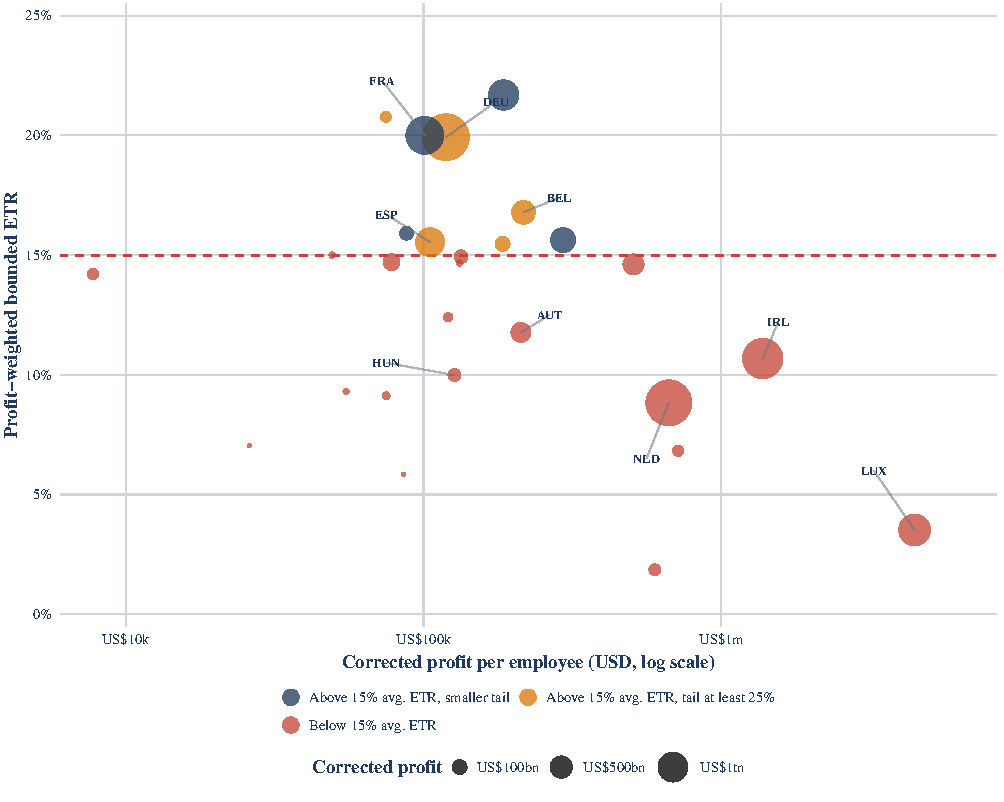
\includegraphics[width=0.96\textwidth]{generated/figures/fig_profit_employee_etr_bubble.pdf}
\caption[Profit per employee and ETRs in EU affiliate jurisdictions.]{Profit per employee and effective tax rates in EU affiliate jurisdictions, 2017--2022. Corrected profit per employee is computed as cumulative corrected positive CbCR profit divided by the corresponding employee count used in the SBIE payroll proxy. The ETR is the profit-weighted bounded Stage 1 ETR. Bubble size is cumulative corrected positive profit. Orange countries have average ETRs above 15\% but distributional low-taxed profit shares of at least 25\%, showing why the distributional branch can identify GMT exposure inside high-average-ETR jurisdictions.}
\label{fig:profit_employee_etr_bubble}
\end{figure}

\subsection{Data limitations and implications for identification}\label{sec:data_limitations}

These limitations define the identification boundary and place the paper in the CbCR-based revenue-estimation literature. Public CbCR improves cross-country coverage but remains anonymised and aggregated by design, which is why the OECD presents it as a monitoring instrument rather than a substitute for confidential tax filings data \citep{oecd2025a}. Firm-level ETR distributions are observed only through bracket and percentile summaries, so the distributional branch follows the same partial-observation logic as the recent low-taxed-profit literature \citep{hugger2026}. CbCR profit before tax differs from GloBE income, and CbCR tax accrued differs from adjusted covered taxes. The correction reduces visible double counting, but it cannot reproduce the full GloBE base or the deferred-tax adjustments discussed in the accounting literature \citep{blouin2023,hanlon2023}. Payroll is proxied, so the SBIE and SBTI layers carry measurement error that is separate from the low-taxed-profit measurement, and this matters because the GMT literature shows that substance relief can materially reduce the effective floor \citep{devereux2023,schjelderup2024}. The sectoral decomposition is therefore an exposure bridge based on FATS and EUKLEMS shares rather than observed sectoral tax liabilities. Finally, the panel is pre-implementation, so behavioural responses, safe-harbour elections and legal allocation outcomes are counterfactual, as in the pre-reform revenue studies that rely on CbCR and simulated rule application \citep{barake2022,boukal2026}. The credible claim is therefore a ranked decomposition of public-data uncertainty. A point estimate alone would overstate what the public data can identify.

The key source-specific bias is aggregation. A jurisdiction-average ETR is informative about the tax system faced by reported profit in that jurisdiction, yet it cannot show whether low-taxed and high-taxed affiliates coexist inside the same country. This is precisely the margin on which jurisdiction-average GMT estimates differ from newer distributional evidence. \citet{barake2022} use jurisdiction-average ETRs and acknowledge that within-country heterogeneity can bias the measured GMT base, while \citet{hugger2026} show that 53.2\% of global low-taxed profit is located in jurisdictions whose average ETR exceeds 15\%. The bias matters directly for the GMT because the reform applies to the low-taxed part of the profit distribution rather than to the jurisdiction average. 

\section{Measurement framework}\label{sec:measurement_framework}

The cleaned CbCR panel from Section \ref{sec:data} provides the accounting inputs needed to approximate GMT revenue. However, the public CbCR needs to be converted into a set of measurement objects that correspond closely to the design of the Global Minimum Tax, which forms the basis of the methodology in Section \ref{sec:methodology}. 

\subsection{Notation and indexing conventions}\label{sec:notation}

The empirical objects are indexed at parent-affiliate-year level. Subscripts $p$, $j$, $s$, $q$ and $t$ denote parent jurisdiction, affiliate or source jurisdiction, collector jurisdiction, sector and fiscal year, with $t \in \{2017,\ldots,2022\}$. Monetary values are in current USD unless stated otherwise. PPP adjustments are not applied to revenue calculations because the GMT applies to nominal profit and tax liabilities. PPP-adjusted wages enter only through the payroll proxy $\hat{W}_{p,j,t}$. Table \ref{tab:notation} collects the recurrent symbols used.

\begin{table}[H]
\centering
\caption{Core Notation for the Revenue Pipeline}
\label{tab:notation}
\footnotesize
\setlength{\tabcolsep}{4pt}
\renewcommand{\arraystretch}{1.00}
\begin{tabularx}{\textwidth}{@{}L{3.15cm}X@{}}
\toprule
Symbol & Meaning in the empirical pipeline \\
\midrule
\multicolumn{2}{@{}l}{\textit{Indices and Scenarios}} \\
$p,j,s,q,t$ & Parent, affiliate/source, collector, sector and fiscal year. \\
$e,a,m,r$ & ETR measurement, substance, behavioural and legal-allocation branches. \\
$\mathbf{x}\in\{0,1\}^5$ & Factorial scenario vector. \\
\addlinespace[2pt]
\multicolumn{2}{@{}l}{\textit{CbCR Inputs and Tax Measures}} \\
$\pi_{p,j,t}$, $\pi^{*}_{p,j,t}$ & Reported profit and corrected positive-profit base. \\
$\theta_{p,j,t}$, $\tau_{p,j,t}$ & Income tax accrued and bounded CbCR ETR, $\theta_{p,j,t}/\pi^{*}_{p,j,t}$. \\
$A_{p,j,t}$, $N_{p,j,t}$, $\hat{W}_{p,j,t}$ & Tangible assets, employees and payroll proxy $N_{p,j,t}\bar{w}_{j,t}$. \\
\addlinespace[2pt]
\multicolumn{2}{@{}l}{\textit{Low-Taxed Base and Substance Shield}} \\
$T$, $F_{j,t}^{e}$ & GMT rate ($0.15$) and profit-weighted ETR distribution under branch $e$. \\
$s_{j,t}^{<T,e}$, $\ell_{p,j,t}^{e}$ & Low-taxed profit share and measured low-taxed profit, $s_{j,t}^{<T,e}\pi^{*}_{p,j,t}$. \\
$\bar{\delta}_{j,t}^{\text{top},e}$, $\lambda_{j,t}^{e}$ & Average top-up gap and pre-SBIE liability rate, $s_{j,t}^{<T,e}\bar{\delta}_{j,t}^{\text{top},e}$. \\
$\sigma_W(t)$, $\sigma_A(t)$ & Payroll and tangible-asset carve-out rates in the SBIE. \\
$\text{SBIE}_{p,j,t}$, $\bar{\phi}_{p,j,t}^{a}$ & Substance exclusion and bounded SBIE-to-profit shield ratio. \\
$\kappa_{j,q,t}$ & Sectoral SBTI-capacity proxy. \\
\addlinespace[2pt]
\multicolumn{2}{@{}l}{\textit{Behaviour, Allocation and Uncertainty}} \\
$\tau_{j,t}^{\text{low},e}$ & Implied ETR of the low-taxed slice, $T-\bar{\delta}_{j,t}^{\text{top},e}$. \\
$\hat{\beta}_{j,t}^{e,m}$, $m_{j,t}^{\text{beh},e,m}$ & Reallocated-profit fraction and behavioural liability filter. \\
$L_{p,j,t}$ & Top-up liability after substance and behaviour, before allocation. \\
$\mathbb{1}_j^{\text{Q}}$, $\mathbb{1}_p^{\text{IIR}}$ & Source-country QDMTT and parent-country IIR status indicators. \\
$\mathbb{1}_s^{\text{UTPR}}$, $\mathbb{1}_p^{\text{SbS}}$ & Collector-country UTPR and parent-country Side-by-Side status indicators. \\
$\omega_{s,p,t}^{\text{U}}$, $a_{s,p,j,t}^{(r)}$ & UTPR collector weight and regime-specific allocation weight. \\
$R_{s,t}(\mathbf{x})$ & Collector-country revenue in scenario $\mathbf{x}$. \\
$\eta_i^2$ & Share of factorial scenario variance attributable to factor $i$. \\
$\mathcal{U}^{A}$, $\mathcal{U}^{B}$, $\mathcal{U}^{C}$ & Scenario, Stage 1 measurement and coefficient-propagation uncertainty. \\
\bottomrule
\end{tabularx}
\end{table}

\subsection{From corrected profit to measurable top-up liability}

The starting point is the corrected positive-profit base $\pi^{*}_{p,j,t}$ from equation \eqref{eq:profit_reconciliation_branch}. This is the public-data denominator after the double-counting correction in Section \ref{sec:doublecounting}. It is indexed by parent jurisdiction $p$, affiliate jurisdiction $j$ and year $t$. The affiliate jurisdiction matters for measuring low-taxed profit and substance. The parent jurisdiction is retained because the allocation rules in Section \ref{sec:sbs} later determine whether source, parent or other implementing jurisdictions collect the top-up tax.

Let $T=0.15$ denote the minimum rate. For each affiliate jurisdiction-year, the ETR source indexed by $e$ measures the part of corrected profit that falls below the threshold. The index $e$ denotes the information source used to measure the same empirical object, ranging from a jurisdiction-average rule to direct Table IV bracket information and distributional imputations where direct support is unavailable. Each branch supplies two quantities. The first is the share of corrected profit taxed below the threshold, $s_{j,t}^{<T,e}$. This converts corrected bilateral profit into measured low-taxed profit:
\begin{equation}\label{eq:lowtax_profit}
\ell_{p,j,t}^{e}=s_{j,t}^{<T,e}\pi^{*}_{p,j,t}.
\end{equation}
The second quantity is the average shortfall from the 15\% floor inside the low-taxed part, $\bar{\delta}_{j,t}^{\text{top},e}$. This gap is needed because low-taxed profit is not the same as liability. A dollar of profit taxed at 14\% and a dollar of profit taxed at 2\% both enter $\ell_{p,j,t}^{e}$, but the second dollar has a much larger top-up gap. The pre-SBIE liability rate on corrected profit is therefore:
\begin{equation}\label{eq:liability_rate}
\lambda_{j,t}^{e}=s_{j,t}^{<T,e}\bar{\delta}_{j,t}^{\text{top},e}.
\end{equation}
Multiplying $\pi^{*}_{p,j,t}$ by $\lambda_{j,t}^{e}$ gives mechanical top-up liability before the substance shield. After the SBIE is applied, the measured liability that enters the behavioural and allocation modules is:
\begin{equation}\label{eq:mechanical_liability}
M_{p,j,t}^{e,a}=\pi^{*}_{p,j,t}\lambda_{j,t}^{e}\left(1-\bar{\phi}_{p,j,t}^{a}\right),
\end{equation}
where $a$ indexes the substance branch and SBIE rate schedule. Equation \eqref{eq:mechanical_liability} is the organising equation for this section: the low-taxed-base step (Stage 1) measures $\lambda_{j,t}^{e}$, the substance-shield step (Stage 2) measures $\bar{\phi}_{p,j,t}^{a}$, and Section \ref{sec:methodology} then adds behavioural reallocation, legal collection rights and the factorial decomposition.

\subsection{Measuring low-taxed profit (Stage 1)}\label{sec:etr_measurement}\label{sec:etr_calc}\label{sec:distributional}

The basic public-data ETR proxy divides current-year income tax accrued by positive corrected pre-tax profit:
\begin{equation}\label{eq:etr}
\tau_{p,j,t}=\frac{\theta_{p,j,t}}{\pi^{*}_{p,j,t}},\quad \pi^{*}_{p,j,t}>0.
\end{equation}
Tax accrued is used because it is the closest public CbCR proxy for current-period covered taxes. This is an approximation: GloBE covered taxes differ from CbCR tax accrued and require legal adjustments that public data cannot reproduce \citep{oecd2025,hanlon2023}. Detailed denominator filters, treatment of negative ETRs, high-ETR caps and percentile conditioning are documented in Appendix \ref{app:measurement_framework}.

A first route compresses all parent-reported profit in affiliate jurisdiction $j$ into one profit-weighted average ETR:
\begin{equation}\label{eq:avg_etr}
\bar{\tau}_{j,t}=\frac{\sum_p \theta_{p,j,t}}{\sum_p \pi^{*}_{p,j,t}}.
\end{equation}
It then applies a binary rule, treating all profit in jurisdiction $j$ as low-taxed only if this average ETR falls below the threshold:
\begin{equation}\label{eq:average_lowtax_share}
s_{j,t}^{<T,\text{avg}}=\mathbb{1}\{\bar{\tau}_{j,t}<T\}.
\end{equation}
This average rule is transparent and close to the first generation of public-data revenue simulations \citep{barake2022}. It asks whether the average jurisdiction is below the floor, while the policy object is the profit mass below the floor. If a jurisdiction has an average ETR of 16\%, equation \eqref{eq:average_lowtax_share} assigns zero low-taxed profit, even if a substantial share of affiliates inside that jurisdiction is taxed below 15\%. \citet{hugger2026} show that 53.2\% of globally low-taxed profit is located in jurisdictions whose average ETR exceeds 15\%.

The distributional route keeps the 15\% threshold but changes the question. Instead of asking whether the average jurisdiction is below the floor, it asks what share of profit inside the jurisdiction is below the floor. Let $F_{j,t}^{e}$ denote the profit-weighted ETR distribution implied by branch $e$, so that $F_{j,t}^{e}(\tau)$ is the share of corrected profit with an ETR no higher than $\tau$. The low-taxed share is:
\begin{equation}\label{eq:lowtax_share}
s_{j,t}^{<T,e}=F_{j,t}^{e}(T).
\end{equation}
The corresponding top-up gap is the average distance to the 15\% floor, conditional on being below the floor:
\begin{equation}\label{eq:topup_gap}
\bar{\delta}_{j,t}^{\text{top},e}=
\begin{cases}
\dfrac{\int_{0}^{T}(T-\tau)\,\mathrm{d}F_{j,t}^{e}(\tau)}{s_{j,t}^{<T,e}} & \text{if } s_{j,t}^{<T,e}>0,\\[8pt]
0 & \text{if } s_{j,t}^{<T,e}=0.
\end{cases}
\end{equation}
The numerator is the missing tax per dollar of corrected profit in the low-taxed tail. Dividing by $s_{j,t}^{<T,e}$ converts that missing-tax mass into the average top-up gap within the tail. Multiplying it back by $s_{j,t}^{<T,e}$ in equation \eqref{eq:liability_rate} gives the unconditional liability rate on corrected profit.

The key empirical choice is how $F_{j,t}^{e}$ is measured. The thesis uses a source hierarchy ordered by information content. Direct Table IV is preferred whenever it is available because it reports subsidiary-level ETR brackets, including the \code{RATE\_0-15} bracket that corresponds to the GMT threshold. Table I percentiles are used where Table IV is absent. Appendix Section \ref{sec:percentile_fit_appendix} fits a bounded, mean-constrained distribution to those percentiles. BSPI shape transport extends distributional support to 2017--2018 by carrying the 2019--2020 Table IV bracket profile backward only where the affiliate profile passes the 2021--2022 hold-out stability test in Appendix Section \ref{sec:bspi}. The jurisdiction-average rule is retained as the fallback when no distributional source exists:
\begin{equation}\label{eq:hybrid}
s_{j,t}^{<T,\text{hyb}} =
\begin{cases}
\dfrac{\pi_{j,t}^{<T,\text{IV}}}{\pi_{j,t}^{\text{all,IV}}} & \text{direct Table IV bracket observation},\\[8pt]
\tilde{F}_{j,t}(T) & \text{Table I percentile fit},\\[4pt]
\bar{s}_{j}^{<T,\text{BSPI}} & \text{validated BSPI shape transport},\\[4pt]
\mathbb{1}\{\bar{\tau}_{j,t}<T\} & \text{jurisdiction-average fallback}.
\end{cases}
\end{equation}
The hierarchy is this section's measurement contribution. It brings the within-jurisdiction insight in \citet{hugger2026} into a public-data revenue framework, while keeping the transparent jurisdiction-average branch used in earlier public simulations as an explicit comparison rather than as the maintained assumption \citep{barake2022}. Each branch estimates the share of profit below 15\% and the corresponding average gap to the floor. Table \ref{tab:stage1_source_updated} reports the realised source assignment. Direct Table IV covers most positive-profit cells after 2019, while the 2017--2018 estimates necessarily rely more heavily on BSPI. This is why the results later report both full-window and higher-measurement-window decompositions.

% Generated by code/13_generate_exhibits.R
\begin{table}[H]
\centering
\small
\setlength{\tabcolsep}{4pt}
\caption[Stage 1 source coverage]{Stage 1 source coverage, 2017 to 2023}
\label{tab:stage1_source_updated}
\begin{tabular}{@{}lrrrrrrrr@{}}
\toprule
Source & 2017 & 2018 & 2019 & 2020 & 2021 & 2022 & 2023 & Total \\
\midrule
Direct Table IV &     0 &     0 & 2,275 & 2,306 & 2,470 & 2,353 & 2,654 & 12,058 \\
Beta percentile fit &     0 &     0 &     0 &     0 &   422 &   399 &   465 &  1,286 \\
BSPI shape transport & 1,720 & 2,179 &     0 &     0 &     0 &     0 &     0 &  3,899 \\
Jurisdiction-average fallback &   303 &   348 &   393 &   408 &     5 &     2 &     3 &  1,462 \\
Missing source &    22 &    27 &    43 &    36 &    25 &    32 &    64 &    249 \\
All analysis pair-years & 2,045 & 2,554 & 2,711 & 2,750 & 2,922 & 2,786 & 3,186 & 18,954 \\
Positive-profit pair-years & 1,554 & 1,932 & 2,026 & 2,011 & 2,259 & 2,090 & 2,236 & 14,108 \\
\bottomrule
\end{tabular}

\vspace{0.35em}
\noindent\begin{minipage}{\textwidth}
\footnotesize\raggedright\textit{Notes:} Counts are parent-affiliate-year cells in the Stage 1 bilateral panel. Positive-profit cells are shown separately because only those cells can generate top-up tax.
\end{minipage}
\end{table}


\subsection{Measuring the substance shield and effective tax floor (Stage 2)}\label{sec:SBIE}\label{sec:floor}\label{sec:payroll_imputation}

After the low-taxed-base measurement, the next question is how much of that liability survives the SBIE. The SBIE is not a tax credit and not a correction to the ETR numerator. It removes a formulaic return on payroll and tangible assets from the base on which the top-up tax is charged. This distinction matters because the headline 15\% minimum is not the effective tax floor on total profit once substance is positive. \citet{devereux2023} show that the SBIE can materially reduce the effective floor for in-scope EU subsidiaries, and \citet{schjelderup2024} formalise the same mechanism as a production-subsidy margin inside Pillar Two.

In the public-data implementation, the bilateral shield is:
\begin{equation}\label{eq:sbie}
\text{SBIE}_{p,j,t}=\sigma_W(t)\hat{W}_{p,j,t}+\sigma_A(t)A_{p,j,t},
\end{equation}
where $\hat{W}_{p,j,t}=N_{p,j,t}\bar{w}_{j,t}$ is the wage-based payroll proxy constructed in Section \ref{sec:substance_data}, and $A_{p,j,t}$ is CbCR tangible assets. Payroll has to be reconstructed because public CbCR reports employees but not current-period payroll. The carve-out rates $\sigma_W(t)$ and $\sigma_A(t)$ are evaluated at the initial transition endpoint and the long-run endpoint in the revenue scenarios. The corresponding shield ratio is:
\begin{equation}\label{eq:sbie_ratio}
\bar{\phi}_{p,j,t}=\min\!\left\{1,\frac{\text{SBIE}_{p,j,t}}{\pi^{*}_{p,j,t}}\right\}.
\end{equation}
This ratio is bounded by one and applied to the pre-substance liability as the excess-profit filter in equation \eqref{eq:mechanical_liability}. It is measured against corrected positive profit, not against low-taxed profit alone, because the public substance inputs are observed at the same bilateral level as corrected profit. 

For intuition, consider a single low-taxed affiliate with pre-reform ETR $\tau_{p,j}<T$ and shield ratio $\phi_{p,j}=\text{SBIE}_{p,j}/\pi_{p,j}$. Total tax after the top-up is:
\begin{equation}\label{eq:total_tax}
\text{Tax} = \underbrace{\tau_{p,j} \cdot \pi_{p,j}}_{\text{local CIT}} + \underbrace{(T - \tau_{p,j}) \cdot (\pi_{p,j} - \text{SBIE}_{p,j})}_{\text{top-up tax}}
\end{equation}

Dividing by profit gives the effective tax rate under Pillar Two:
\begin{equation}\label{eq:etr_pillar2}
\tau_{p,j}^{\text{P2}} = T - (T - \tau_{p,j}) \cdot \frac{\text{SBIE}_{p,j}}{\pi_{p,j}} = T - \delta_{p,j}^{\text{top}} \cdot \phi_{p,j}
\end{equation}
\begin{figure}[H]
\centering
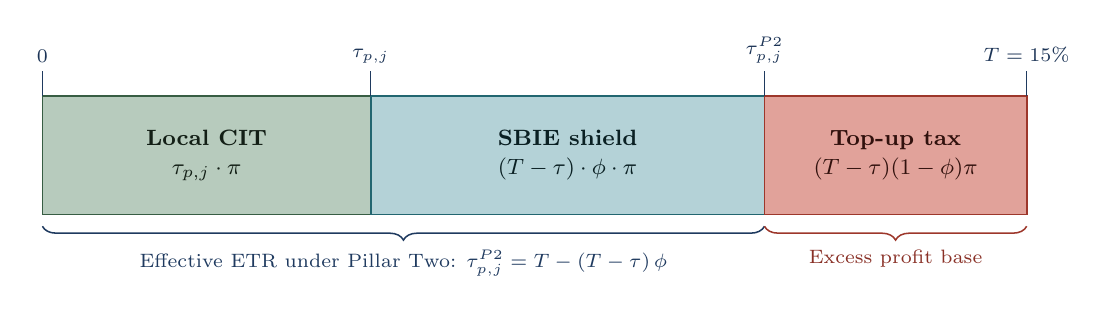
\begin{tikzpicture}[font=\small]
  \def\W{12.5}
  \def\H{1.5}
  \def\xa{4.17}
  \def\xb{9.17}

  \fill[thesisLight] (0,0) rectangle (\W,\H);

  \fill[thesisGreen!40, draw=thesisGreen!75!black, line width=0.6pt] (0,0) rectangle (\xa, \H);
  \node[font=\footnotesize, align=center, thesisGreen!25!black]
    at (\xa/2, \H/2) {\textbf{Local CIT}\\[1pt]$\tau_{p,j}\cdot\pi$};

  \fill[thesisTeal!35, draw=thesisTeal!80!black, line width=0.6pt] (\xa,0) rectangle (\xb, \H);
  \node[font=\footnotesize, align=center, thesisTeal!25!black]
    at ({(\xa+\xb)/2}, \H/2) {\textbf{SBIE shield}\\[1pt]$(T-\tau)\cdot\phi\cdot\pi$};

  \fill[thesisRed!50, draw=thesisRed!80!black, line width=0.6pt] (\xb,0) rectangle (\W, \H);
  \node[font=\footnotesize, align=center, thesisRed!25!black]
    at ({(\xb+\W)/2}, \H/2) {\textbf{Top-up tax}\\[1pt]$(T-\tau)(1-\phi)\pi$};

  \draw[thesisNavy, line width=0.5pt] (0, \H) -- (0, \H+0.32);
  \draw[thesisNavy, line width=0.5pt] (\xa, \H) -- (\xa, \H+0.32);
  \draw[thesisNavy, line width=0.5pt] (\xb, \H) -- (\xb, \H+0.32);
  \draw[thesisNavy, line width=0.5pt] (\W, \H) -- (\W, \H+0.32);
  \node[above, font=\scriptsize, thesisNavy!90!black] at (0, \H+0.30) {$0$};
  \node[above, font=\scriptsize, thesisNavy!90!black] at (\xa, \H+0.30) {$\tau_{p,j}$};
  \node[above, font=\scriptsize, thesisNavy!90!black] at (\xb, \H+0.30) {$\tau^{P2}_{p,j}$};
  \node[above, font=\scriptsize, thesisNavy!90!black] at (\W, \H+0.30) {$T = 15\%$};

  \draw[decorate, decoration={brace, mirror, amplitude=5pt}, thesisNavy, line width=0.55pt]
    (0,-0.15) -- node[below=5pt, font=\scriptsize]
    {Effective ETR under Pillar Two: $\tau^{P2}_{p,j} = T - (T-\tau)\,\phi$} (\xb,-0.15);

  \draw[decorate, decoration={brace, mirror, amplitude=5pt}, thesisRed!80!black, line width=0.55pt]
    (\xb,-0.15) -- node[below=5pt, font=\scriptsize, thesisRed!70!black] {Excess profit base} (\W,-0.15);
\end{tikzpicture}
\caption[Effective Pillar Two tax floor.]{Decomposition of taxable profit at the 15\% threshold for a low-tax MNE affiliate. Local corporate income tax collects $\tau_{p,j}\pi$. The SBIE shields a fraction $\phi=\text{SBIE}/\pi$ of the gap to the headline rate, leaving only the residual excess-profit base on which the top-up tax is levied.}
\label{fig:effective_floor}
\end{figure}

Equation \eqref{eq:etr_pillar2} shows the tax concept in one line. The effective floor equals the headline floor minus the part of the top-up gap that is shielded by payroll and tangible assets. The gap is larger when the pre-reform ETR is further below 15\% and when the SBIE-to-profit ratio is larger.

\subsection{Sectoral substance and SBTI exposure}\label{sec:sbti_amplification}\label{sec:sbti}\label{sec:sbie_decomp}

The aggregate SBIE shield can hide large sector differences. Manufacturing cells generally have more payroll and tangible assets relative to profit than holding or intellectual-property cells, so the same headline floor can imply different effective floors across sectors \citep{devereux2023,schjelderup2024}. The sectoral branch keeps the CbCR country-level liability base fixed and uses Eurostat FATS and EUKLEMS shares only to allocate payroll, tangible assets and profit across EU host-country sectors \citep{eurostat2025fats,euklemsintanprod2025}. Appendix \ref{app:sector} documents the bridge and its coverage thresholds.

For sector $q$ in jurisdiction $j$, the sectoral shield ratio later used in the revenue scenarios:
\begin{equation}\label{eq:rho_sector}
\phi_{j,q,t}=\sigma_W(t)\frac{W_{j,q,t}}{\pi_{j,q,t}}+\sigma_A(t)\frac{A_{j,q,t}}{\pi_{j,q,t}}.
\end{equation}
The country-level ratio is the profit-weighted sector average:
\begin{equation}\label{eq:rho_sectoral}
\phi_{j,t}=\sum_q\omega_{j,q,t}\phi_{j,q,t},\quad \omega_{j,q,t}=\frac{\pi_{j,q,t}}{\pi_{j,t}}.
\end{equation}

The January 2026 SBTI Safe Harbour adds a related but distinct exposure margin. It can protect qualifying tax incentives up to a substance-linked cap \citep{oecd2026}. The SBIE reduces the excess-profit base. The SBTI can increase covered taxes by allowing qualifying incentives to be treated favourably up to the cap. Public data do not observe actual qualifying tax incentives, safe-harbour elections or the legal classification of local credits. The empirical object is therefore an exposure index. The SBTI-capacity proxy normalises the public-data approximation of the cap by profit:
\begin{equation}\label{eq:sbti_capacity}
\kappa_{j,q,t} = \frac{\max\!\left(0.055\,W_{j,q,t},\; 0.01\,A_{j,q,t}\right)}{\pi_{j,q,t}}
\end{equation}
The legal cap and the public-data simplification behind equation \eqref{eq:sbti_capacity} are derived in Appendix \ref{app:sbti_details}. In the main estimates, $\kappa_{j,q,t}$ measures capacity. A high value means that a sector-country cell has enough payroll or tangible assets relative to profit to shelter qualifying incentives if such incentives exist. A low value means that the SBTI channel is unlikely to matter even if the jurisdiction offers tax incentives, because there is little substance against which the legal cap can be computed.

\section{Methodology}\label{sec:methodology}

This chapter turns the measured CbCR inputs into EU collector-country revenue estimates. It first estimates how reported profit responds when effective tax rates change, because the revenue counterfactual depends on how much profit remains in low-tax jurisdictions once the 15\% floor binds. It then applies the legal order of QDMTTs, IIRs, UTPRs and the Side-by-Side safe harbour to assign collection rights over the remaining top-up tax.

The final step combines the measurement, substance, behavioural and allocation choices into a 32-scenario revenue matrix. That matrix is used to decompose the spread across estimates and to group Member States with similar exposure patterns. The method therefore follows the revenue calculation itself: define the low-taxed base, adjust it for substance and behaviour, allocate the residual liability, and identify which choices drive uncertainty.

\subsection{Panel estimation of profit-shifting semi-elasticities}\label{sec:estimation}

The policy question is simple: if the GMT raises the effective tax rate faced by low-taxed affiliates, how much reported profit should remain in those affiliates? The answer is governed by a tax semi-elasticity. A semi-elasticity of one means that a one percentage-point increase in the ETR is associated with about one per cent lower reported profit, conditional on the controls and fixed effects in the model. 

The estimation uses the Hines--Rice logic that reported profit in a jurisdiction reflects both real activity and the tax incentive to book income there \citep{hines1994}. The usual cross-sectional risk is that low-tax jurisdictions differ from high-tax jurisdictions in persistent ways. A pure comparison of Luxembourg and Germany, for example, would mix tax incentives with treaty networks, sector composition, legal infrastructure and headquarters patterns. The panel design instead compares changes within the same parent-affiliate relationship over time. Parent--affiliate fixed effects absorb time-invariant bilateral differences, while year fixed effects absorb common shocks.

\subsubsection{Estimation framework}\label{sec:hines_rice}

Reported pre-tax profit in affiliate jurisdiction $j$ of parent $p$ in year $t$ is modelled as a function of real activity and the local tax rate:
\begin{equation}\label{eq:panel_linear}
\log \pi_{p,j,t}^{*} = \beta_0 + \beta_1 \log A_{p,j,t} + \beta_2 \log \hat{W}_{p,j,t} + \beta_3 \, \tau_{p,j,t} + \mathbf{\beta}_x \mathbf{X}_{p,j,t} + \alpha_{pj} + \gamma_t + \varepsilon_{p,j,t}
\end{equation}
where $\pi^{*}$ is corrected profit (Section \ref{sec:doublecounting}), $A$ is tangible assets, $\hat{W}$ is the wage-based payroll proxy (Section \ref{sec:payroll_imputation}), $\tau$ is the CbCR effective tax rate, $\alpha_{pj}$ is a parent--affiliate fixed effect and $\gamma_t$ is a year fixed effect. The vector $\mathbf{X}$ contains log GDP per capita and log population of the affiliate jurisdiction. With $\tau$ expressed as a unit rate, $-\beta_3$ is the semi-elasticity per percentage point. Tangible assets and payroll are included because the Hines--Rice estimand is the tax sensitivity of reported profit conditional on real activity.

The first modelling risk is functional form. A linear response applies the same semi-elasticity at an ETR of 4\% as at an ETR of 24\%. That may be too restrictive because profit shifting is concentrated at very low tax rates. Following \citet{dowd2017}, the quadratic specification allows the slope to vary with the tax rate:
\begin{equation}\label{eq:panel_quadratic}
\log \pi_{p,j,t}^{*} = \beta_0 + \beta_1 \log A_{p,j,t} + \beta_2 \log \hat{W}_{p,j,t} + \beta_3 \, \tau_{p,j,t} + \beta_4 \, \tau_{p,j,t}^2 + \mathbf{\beta}_x \mathbf{X}_{p,j,t} + \alpha_{pj} + \gamma_t + \varepsilon_{p,j,t}
\end{equation}
The implied semi-elasticity varies with the ETR: $\varepsilon(\tau) = \beta_3 + 2\beta_4 \tau$.

Following \citet{garcia-bernardo2024}, the logarithmic specification allows a sharper response close to zero:
\begin{equation}\label{eq:panel_log}
\log \pi_{p,j,t}^{*} = \beta_0 + \beta_1 \log A_{p,j,t} + \beta_2 \log \hat{W}_{p,j,t} + \beta_3 \, \tau_{p,j,t} + \beta_4 \log(t_0 + \tau_{p,j,t}) + \mathbf{\beta}_x \mathbf{X}_{p,j,t} + \alpha_{pj} + \gamma_t + \varepsilon_{p,j,t}
\end{equation}
where $t_0$ is a small offset selected by minimising the BIC over the grid $t_0 \in [0.001, 0.200]$, in line with \citep{garcia-bernardo2024}. The implied semi-elasticity is $\varepsilon(\tau) = \beta_3 + \beta_4/(t_0+\tau)$. The BIC ranks the three models on the common estimation sample, and the Vuong test compares the two non-nested nonlinear alternatives. Appendix \ref{app:behavioural_details} gives the functional-form mappings and Figure \ref{fig:semi_elasticity_forms} shows the implied curve shapes.

\subsubsection{Identification}\label{sec:identification}

Identifying variation comes from within-pair movement in the CbCR ETR over 2017--2022. The pair fixed effect $\alpha_{pj}$ absorbs persistent bilateral features, including treaty access, distance, language, legal-system similarity and stable MNE group structure. The year fixed effect $\gamma_t$ absorbs common shocks. This follows the panel version of the Hines--Rice design, where fixed effects reduce bias from time-invariant unobserved profitability differences and the tax coefficient is identified from changes within units rather than from levels across low- and high-tax locations \citep{dharmapala2014,heckemeyer2017}. 

Affiliate-clustered standard errors are retained as a one-way diagnostic for host-country shocks. Model selection proceeds in two stages. The BIC ranks the linear, quadratic and logarithmic specifications on the common sample. A \citet{vuong1989} test then compares the two non-nested nonlinear specifications through their observation-level log-likelihoods.

The remaining concern is mechanical tax endogeneity. The CbCR ETR equals tax accrued divided by reported profit, so profit shifting can affect the dependent variable and the tax denominator simultaneously. CbCR definitions of profit and current-year tax accrued can distort ETRs when dividends, equity income, loss offsets or timing differences affect the denominator and numerator asymmetrically \citep{bobeldijk2019,blouin2023}. The fixed-effect coefficient serves as the preferred behavioural input because it uses the full public panel. 

\subsubsection{Instrumental-variable robustness}\label{sec:iv_strategy}

To isolate tax variation that is less mechanically tied to current-year reported profit, the IV diagnostic uses the OECD forward-looking effective average tax rate for a fixed composite investment project in affiliate jurisdiction $j$ and year $t$, denoted $z_{j,t}^{\text{sim}}$. This simulated EATR holds the investment project fixed and varies the tax-code environment: statutory rates, allowances and other rules embedded in the OECD model. The one-year lagged statutory CIT rate, $z_{j,t-1}^{\text{CIT}}$, is retained as a benchmark because it is predetermined with respect to current-year reporting.

The first stage is:
\begin{equation}\label{eq:iv_first_stage}
\tau_{p,j,t} = \pi_0 + \pi_1 z_{j,t}^{\text{IV}} + \pi_2 \log A_{p,j,t} + \pi_3 \log \hat{W}_{p,j,t} + \mathbf{\pi}_x \mathbf{X}_{j,t} + \alpha_{pj} + \gamma_t + \nu_{p,j,t},
\end{equation}
where $z_{j,t}^{\text{IV}}$ is estimated separately as $z_{j,t}^{\text{sim}}$ and $z_{j,t-1}^{\text{CIT}}$.
The second stage replaces the potentially endogenous CbCR ETR in the linear Hines--Rice equation with the first-stage fitted value:
\begin{equation}\label{eq:iv_second_stage}
\log \pi_{p,j,t}^{*} = \beta_0^{\text{IV}} + \beta_1^{\text{IV}} \log A_{p,j,t} + \beta_2^{\text{IV}} \log \hat{W}_{p,j,t} + \beta_3^{\text{IV}} \widehat{\tau}_{p,j,t} + \mathbf{\beta}_x^{\text{IV}} \mathbf{X}_{j,t} + \alpha_{pj} + \gamma_t + \varepsilon_{p,j,t}^{\text{IV}}.
\end{equation}
The reduced form is estimated in parallel by replacing $\tau_{p,j,t}$ in \eqref{eq:iv_second_stage} with each excluded instrument. A useful instrument should have a relevant first stage and a same-signed reduced form. The identifying assumption remains demanding, since tax reforms can respond to fiscal pressure or avoidance activity. The IV estimates are therefore reported as credibility diagnostics for the linear tax coefficient. Extending the IV design to the quadratic or logarithmic specifications would require separate excluded instruments for nonlinear tax terms and a multivariate weak-instrument assessment, which the public CbCR panel cannot support credibly.

\subsubsection{Robustness checks}\label{sec:estimation_robustness}
Five robustness checks are implemented on the the behavioural estimate. The balanced-panel check tests whether expanding CbCR coverage over time drives the coefficient. The wage-quality check examines whether stale wage proxies distort the payroll control. The pandemic exclusion removes 2020--2021 to test whether profit compression in those years alters the tax coefficient. The cluster comparison contrasts host-country-only clustering against two-way clustering to assess whether inference is driven by a single side of the bilateral structure. The FE-2SLS diagnostics test whether tax-code variation supports the fixed-effect association. A lower-tail support diagnostic assesses whether nonlinear terms are identified where the GMT bites most, below an ETR of 5 per cent. The jurisdiction-influence exercise drops one major parent or affiliate jurisdiction at a time, refits the Stage 3 model, recomputes the Stage 1 liability rate and rebuilds the EU revenue decomposition to check whether the ranking of uncertainty channels depends on a single dominant country. The full-sample estimate remains preferred because large jurisdictions are part of the policy population.

\subsection{Behavioural counterfactual response}\label{sec:behavioural}

The behavioural estimate has to be translated into the object used by a revenue model. The tax floor raises the ETR on the low-taxed slice from its measured value to 15\%, and the semi-elasticity predicts the fraction of reported profit that remains in that slice. This creates the liability filter $m_{j,t}^{\text{beh}}$ in equation \eqref{eq:pipeline}. The filter has two margins. The estimated margin applies the BIC-preferred linear semi-elasticity below the safe-harbour band. The safe-harbour margin sets top-up liability to zero in a narrow band below 15\%, reflecting the Simplified ETR Safe Harbour (SESH) introduced in the January 2026 \citep{oecd2026}.

\subsubsection{From semi-elasticity estimates to the reallocation factor}\label{sec:reallocation_mapping}

For each ETR measurement branch, Stage 1 supplies the profit-weighted average top-up rate on the low-taxed slice, $\bar{\delta}_{j,t}^{\text{top},e}$. The implied ETR of the profit that enters the GMT base is:
\begin{equation}\label{eq:tau_low_segment}
\tau_{j,t}^{\text{low},e} = T - \bar{\delta}_{j,t}^{\text{top},e}
\end{equation}
With $\hat{\beta}_3<0$ from the linear Hines--Rice model, the counterfactual profit ratio when the low-taxed slice is raised to $T$ is:
\begin{equation}\label{eq:cf_linear}
G_{\text{lin}}(\tau) = \exp\!\left[\hat{\beta}_3\,(T-\tau)\right]
\end{equation}
Reallocation is active only when the branch identifies a positive low-taxed share and a positive top-up rate. The affiliate-year response is bounded to the unit interval and looks the following:
\begin{equation}\label{eq:beta_aggregated}
\hat{\beta}_{j,t}^{e,m}
\;=\;
\mathbf{1}\{s_{j,t}^{<T,e}>0,\ \bar{\delta}_{j,t}^{\text{top},e}>0\}
\cdot \left[1-G_{\text{lin}}\!\left(\tau_{j,t}^{\text{low},e}\right)\right]
\end{equation}
In the final revenue matrix this response applies only to bilateral rows with positive post-SBIE low-taxed profit and legal collection exposure. 

\subsubsection{Safe-harbour regime and bunching under the Simplified ETR Safe Harbour}\label{sec:bunching}\label{sec:sesh}

The Simplified ETR Safe Harbour (SESH) means that an affiliate jurisdiction whose simplified ETR reaches 15\% has its top-up tax deemed zero and avoids the full GloBE computation for that jurisdiction \citep{oecd2026}. The revenue model therefore uses an upper-bound filter: 
\begin{equation}\label{eq:regime}
m_{j,t}^{\text{beh},e,m} = \begin{cases}
0 & \text{if } \tau_{j,t}^{\text{low},e} \in [T - \eta,\; T), \\[2pt]
1-\hat{\beta}_{j,t}^{e,m} & \text{if } \tau_{j,t}^{\text{low},e} < T - \eta, \\[2pt]
1 & \text{otherwise.}
\end{cases}
\end{equation}
where $T = 0.15$ and the baseline bandwidth is $\eta = 0.02$. Inside the band $[T-\eta,T)$, pre-tax profit stays in place and top-up liability is set to zero. Below the band, the semi-elasticity response in \eqref{eq:beta_aggregated} applies. Appendix \ref{app:sesh_details} records the structural bunching logic and the pre-reform density diagnostic.

\subsubsection{Redistribution of reallocated profit}\label{sec:reallocation}

The reallocated profit is assigned to destination jurisdictions. The thesis adopts the formulary reallocation of \citet{garcia-bernardo2024}:
\begin{equation}\label{eq:reallocation}
R_i = \tfrac{1}{4}\frac{N_i}{\sum_{k} N_k} + \tfrac{1}{4}\frac{W_i}{\sum_{k} W_k} + \tfrac{1}{2}\frac{\text{UPR}_i}{\sum_{k} \text{UPR}_k},
\end{equation}
with $N_i$ employment, $W_i$ payroll, and $\text{UPR}_i$ unrelated-party revenue of MNE activity in destination $i$. Summation is restricted to destinations with $\tau_{i,t} \geq T$ so that reallocated profit is not mechanically re-deposited in a second haven.

Redistribution does not itself generate EU top-up revenue. An additional euro sent to a jurisdiction with $\tau_{i,t}\ge T$ enters above the floor and contributes zero to the GMT top-up. Equation \eqref{eq:reallocation} therefore verifies profit conservation and checks whether the implied re-reporting pattern aligns with real activity. The SBIE is evaluated on pre-response payroll and tangible assets. This keeps the short-run reported-profit response separate from the longer-run real-activity response documented in \citet{bilicka2022} and \citet{suarezserrato2018}. Additional uncertainty is quantified in Appendix \ref{sec:beta_uncertainty}, which separates coefficient uncertainty from scenario spread and explains why the factorial behavioural contrast should not be read as a confidence interval.

\subsection{Revenue allocation and the Side-by-Side Safe Harbour}\label{sec:sbs}\label{sec:jan2026}

The previous steps compute how much top-up tax exists. The allocation step decides which government can collect it. The source-country top-up tax, labelled QDMTT in the legal rules, gives the host jurisdiction first collection rights. If the source country has no qualified domestic top-up, the parent-country backstop, the IIR, collects the residual. If source and parent collection are unavailable, the enforcement backstop, the UTPR, assigns liability to implementing jurisdictions using substance weights.

The January 2026 Side-by-Side (SbS) Safe Harbour changes this rule order for qualifying parent jurisdictions \citep{oecd2026}. MNE groups headquartered in a jurisdiction with a ``Qualified SbS Regime'' (currently only the United States) may elect a deemed top-up tax of zero under both the IIR and the UTPR \citep{oecdCentralRecord2026, oecd2026}.\footnote{The SbS Safe Harbour could be extended to more countries in the near future.} US-parented MNEs are therefore outside residual IIR and UTPR collection in the SbS scenario. QDMTTs remain operative under the SbS Safe Harbour. The SbS package therefore creates a sharp discontinuity: for US-parented MNEs, the IIR and UTPR channels are switched off, while the QDMTT channel remains operational.

The source-level waterfall assigns this liability to four mutually exclusive pools. The first pool is collected by the source jurisdiction $j$ through a QDMTT. The second is collected by the parent jurisdiction $p$ through the IIR. The third is a UTPR pool. The fourth is not revenue. It is the liability extinguished by the SbS election after the source jurisdiction has declined, or lacks, a QDMTT. Under the universal regime $\mathbb{1}_p^{\text{SbS}}=0$ for all parents. Under the SbS regime it equals one for qualified US-parented groups. Let $L_{p,j,t}$ denote the post-behaviour, pre-allocation top-up liability from equation \eqref{eq:pipeline}:
\begin{align}
L_{p,j,t}^{\text{Q}} &= \mathbb{1}_j^{\text{Q}} L_{p,j,t}, \label{eq:qdmtt_sbs} \\
L_{p,j,t}^{\text{I}} &= (1-\mathbb{1}_j^{\text{Q}})\mathbb{1}_p^{\text{IIR}}(1-\mathbb{1}_p^{\text{SbS}})L_{p,j,t}, \label{eq:iir_sbs} \\
L_{p,j,t}^{\text{U}} &= (1-\mathbb{1}_j^{\text{Q}})(1-\mathbb{1}_p^{\text{IIR}})(1-\mathbb{1}_p^{\text{SbS}})L_{p,j,t}, \label{eq:utpr_sbs} \\
L_{p,j,t}^{\text{S}} &= (1-\mathbb{1}_j^{\text{Q}})\mathbb{1}_p^{\text{SbS}}L_{p,j,t}. \label{eq:sbs_extinguish}
\end{align}

The UTPR pool is  allocated to implementing collector jurisdictions $s$ using parent-year substance weights built from the public CbCR employee and tangible-asset variables:
\begin{equation}\label{eq:utpr_weight}
\omega_{s,p,t}^{\text{U}}
=
\frac{
\mathbb{1}_s^{\text{UTPR}}
\left[
\tfrac{1}{2}\frac{N_{p,s,t}}{\sum_{h:\mathbb{1}_h^{\text{UTPR}}=1}N_{p,h,t}}
+
\tfrac{1}{2}\frac{A_{p,s,t}}{\sum_{h:\mathbb{1}_h^{\text{UTPR}}=1}A_{p,h,t}}
\right]
}{
\sum_{h:\mathbb{1}_h^{\text{UTPR}}=1}
\left[
\tfrac{1}{2}\frac{N_{p,h,t}}{\sum_{r:\mathbb{1}_r^{\text{UTPR}}=1}N_{p,r,t}}
+
\tfrac{1}{2}\frac{A_{p,h,t}}{\sum_{r:\mathbb{1}_r^{\text{UTPR}}=1}A_{p,r,t}}
\right]
}.
\end{equation}
If only the employee or asset denominator is available, the implemented weight uses the available share alone. If no parent-year collector activity is available, the code falls back to a global year-level UTPR weight. Collector revenue is therefore:
\begin{align}
R_{s,t}^{\text{QDMTT}} &= \sum_p \sum_j \mathbb{1}\{s=j\}L_{p,j,t}^{\text{Q}}, \\
R_{s,t}^{\text{IIR}} &= \sum_p \sum_j \mathbb{1}\{s=p\}L_{p,j,t}^{\text{I}}, \\
R_{s,t}^{\text{UTPR}} &= \sum_p \sum_j \omega_{s,p,t}^{\text{U}}L_{p,j,t}^{\text{U}}.
\end{align}

\begin{figure}[H]
\centering
\resizebox{\textwidth}{!}{%
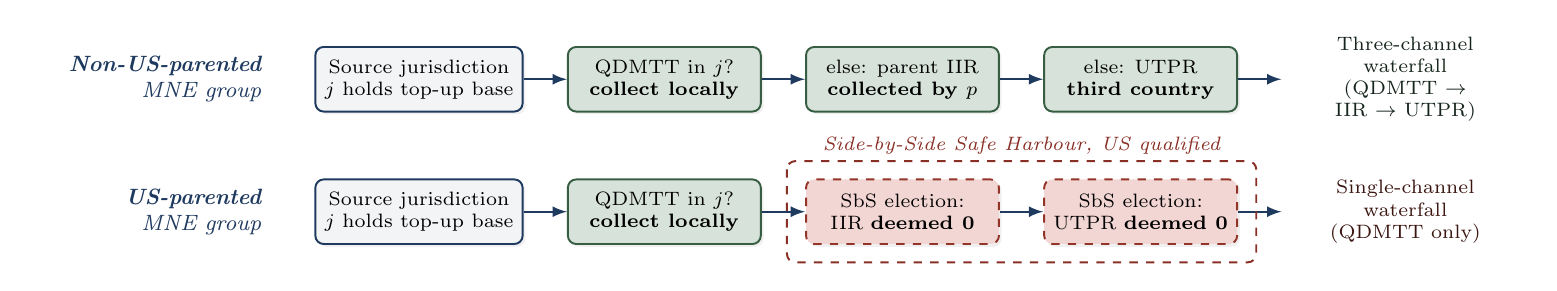
\begin{tikzpicture}[font=\small, node distance=0.55cm and 0.55cm,
    rule/.style={draw=thesisNavy, line width=0.7pt, rounded corners=3pt,
                 fill=thesisLight, minimum width=2.45cm, minimum height=0.82cm,
                 align=center, font=\scriptsize,
                 drop shadow={shadow xshift=1pt, shadow yshift=-1pt, opacity=0.12}},
    label/.style={font=\footnotesize\itshape, thesisNavy, align=right,
                  text width=2.85cm},
    outcome/.style={font=\scriptsize, align=center, text width=2.9cm},
    on/.style={fill=thesisGreen!22, draw=thesisGreen!75!black},
    off/.style={fill=thesisRed!22, draw=thesisRed!75!black, dashed}]

  % Non-US lane
  \node[label] (h1) {\textbf{Non-US-parented}\\MNE group};
  \node[rule, right=0.55cm of h1] (sl) {Source jurisdiction\\$j$ holds top-up base};
  \node[rule, on, right=of sl] (q1) {QDMTT in $j$?\\\textbf{collect locally}};
  \node[rule, on, right=of q1] (i1) {else: parent IIR\\\textbf{collected by $p$}};
  \node[rule, on, right=of i1] (u1) {else: UTPR\\\textbf{third country}};
  \node[outcome, thesisGreen!30!black, right=0.55cm of u1] (o1)
    {Three-channel\\waterfall\\(QDMTT $\to$ IIR $\to$ UTPR)};

  % US lane
  \node[label, below=0.85cm of h1] (h2) {\textbf{US-parented}\\MNE group};
  \node[rule, right=0.55cm of h2] (sr) {Source jurisdiction\\$j$ holds top-up base};
  \node[rule, on, right=of sr] (q2) {QDMTT in $j$?\\\textbf{collect locally}};
  \node[rule, off, right=of q2] (i2) {SbS election:\\IIR \textbf{deemed 0}};
  \node[rule, off, right=of i2] (u2) {SbS election:\\UTPR \textbf{deemed 0}};
  \node[outcome, thesisRed!30!black, right=0.55cm of u2] (o2)
    {Single-channel\\waterfall\\(QDMTT only)};

  % Arrows
  \foreach \a/\b in {sl/q1, q1/i1, i1/u1, u1/o1} \draw[thesis arrow] (\a) -- (\b);
  \foreach \a/\b in {sr/q2, q2/i2, i2/u2, u2/o2} \draw[thesis arrow] (\a) -- (\b);

  % SbS exemption band over the affected steps
  \draw[thesisRed!70!black, line width=0.7pt, rounded corners=3pt, dashed]
    ([xshift=-0.23cm, yshift=0.22cm]i2.north west) rectangle
    ([xshift=0.23cm, yshift=-0.22cm]u2.south east);
  \node[font=\scriptsize\itshape, thesisRed!70!black, align=center]
    at ($(i2.north)!0.5!(u2.north) + (0, 0.42)$)
    {Side-by-Side Safe Harbour, US qualified};

\end{tikzpicture}
}
\caption[Allocation rule under the Side-by-Side Safe Harbour.]{Collection waterfall under the original GloBE rule order versus the January 2026 Side-by-Side Safe Harbour.}
\label{fig:sbs_waterfall}
\end{figure}

\subsection{Counterfactual revenue equation}\label{sec:pipeline}

For each bilateral parent--affiliate cell, the pre-allocation top-up liability is built up multiplicatively: a euro of corrected profit is scaled by the low-taxed share and the average top-up rate on that slice, then reduced by the SBIE shield, and finally passed through the behavioural liability filter before being routed to the collecting jurisdiction.\footnote{The components draw on \citet{hugger2026} for low-taxed-profit measurement, \citet{schjelderup2024} and \citet{devereux2023} for the substance filter, and the panel-estimated semi-elasticities in Section \ref{sec:estimation} for the behavioural counterfactual.}
\begin{equation}\label{eq:pipeline}
L_{p,j,t} = \underbrace{\ell_{p,j,t} \cdot \bar{\delta}_{j,t}^{\text{top}}}_{\text{ETR measurement}} \times \underbrace{\left(1 - \bar{\phi}_{p,j,t}\right)}_{\text{SBIE measurement}} \times \underbrace{m_{j,t}^{\text{beh}}}_{\text{behavioural counterfactual}}
\end{equation}
where $\ell_{p,j,t} = s_{j,t}^{<T} \cdot \pi_{p,j,t}^{*}$ is low-taxed profit (Section \ref{sec:etr_measurement}), $\bar{\delta}_{j,t}^{\text{top}}$ is the average top-up rate on that low-taxed portion, $\bar{\phi}_{p,j,t}$ is the SBIE shield (Section \ref{sec:SBIE}), and $m_{j,t}^{\text{beh}}$ is the behavioural liability filter defined in \eqref{eq:regime}, with ETR-measurement and semi-elasticity-model superscripts suppressed. The allocation rule then distributes the liability:
\begin{equation}\label{eq:allocation}
R_{s,t}^{(r)} = \sum_p \sum_j a_{s,p,j,t}^{(r)} \cdot L_{p,j,t}
\end{equation}
where $a_{s,p,j,t}^{(r)}$ is the regime-specific allocation weight implied by the QDMTT/IIR/UTPR rule order under policy regime $r$ (Section \ref{sec:sbs}). For UTPR liabilities, $a_{s,p,j,t}^{(r)}$ is the parent-year substance weight in \eqref{eq:utpr_weight}, or the global year-level fallback where no parent-year collector key is available.

Revenue uncertainty compounds. A positive ETR-measurement $\times$ SBIE interaction indicates that the distributional approach uncovers low-taxed profit concentrated in capital-intensive sectors with a large $\phi$, so the expanded base is partially offset by stronger SBIE shielding. The equation also identifies the highest-return data improvement. If ETR measurement dominates, within-jurisdiction ETR data from confidential CbCR microdata are the priority. If SBIE measurement dominates, better CbCR coverage of tangible assets and payroll matters more.

\subsection{Counterfactual decomposition}\label{sec:decomposition}

The decomposition targets a concrete question: why do reasonable GMT revenue estimates differ? Five binary choices are toggled simultaneously in the revenue equation: how the low-taxed base is measured, how substance is measured, which SBIE rate applies, which government holds collection rights, and whether reported profit responds to the tax floor. Toggling five binary choices yields 32 scenarios. The decomposition then attributes the spread across scenarios to its constituent sources.

\subsubsection{Factor definitions}\label{sec:factors}

Table \ref{tab:factors} defines the five choices. 

\begin{table}[H]
\centering
\caption{Scenario factors in the decomposition}
\label{tab:factors}
\small
\begin{tabular}{@{}clp{3.8cm}p{3.8cm}@{}}
\toprule
Factor & Choice & Low level ($x_i = 0$) & High level ($x_i = 1$) \\
\midrule
1 & Low-taxed-base measurement & Jurisdiction-average ETR rule & Distributional low-taxed share from the hybrid branch \\
2 & Substance specification & Aggregate public-CbCR SBIE & EU sectoral bridge with SBTI-capacity overlay ($\kappa$) \\
3 & SBIE rates & Initial transition rates (10\% payroll, 8\% assets) & Long-run rates (5\%, 5\%) \\
4 & Allocation regime & Universal IIR and UTPR collection & SbS regime for qualified US-parented groups \\
5 & Behavioural filter & Mechanical revenue, no reallocation & Linear semi-elasticity plus SESH liability filter \\
\bottomrule
\end{tabular}
\end{table}

Factor 1 changes the measured low-taxed share $s_j^{<T}$. Factor 2 changes the substance shield $\bar{\phi}_{p,j,t}$ by imposing an EU host-country sectoral bridge and the SBTI-capacity index from equation \eqref{eq:sbti_capacity}. Factor 3 changes the policy parameters in the SBIE. Factor 4 changes the allocation weight $a_{s,p,j,t}^{(r)}$ by switching residual IIR and UTPR collection off for qualified US-parented groups while leaving QDMTTs operative. Factor 5 replaces the mechanical filter with $m_{j,t}^{\text{beh}}$.

Let $\mathbf{x} = (x_1,\ldots,x_5) \in \{0,1\}^5$ denote a scenario configuration. The revenue of EU collector country $s$ in year $t$ is $R_{s,t}(\mathbf{x})$. The design is balanced, so the scenario spread can be decomposed exactly with orthogonal contrasts. The algebra follows an ANOVA table. For $K=5$ factors, $\text{SS}_i$ is the main effect of factor $i$, $\text{SS}_{ik}$ is the two-way interaction between factors $i$ and $k$, and higher-order terms are defined analogously. With five binary factors, the decomposition yields 31 orthogonal contrasts that exhaust the total variation:
\begin{equation}\label{eq:anova}
\text{SS}_{\text{total}} = \sum_{i=1}^{5} \text{SS}_i + \sum_{i<k} \text{SS}_{ik} + \sum_{i<k<l} \text{SS}_{ikl} + \cdots + \text{SS}_{12345}
\end{equation} 

Each effect is computed from the orthogonal contrast in the balanced design. For a main effect of factor $i$ where $\bar{R}_{x_i = 1}$ and $\bar{R}_{x_i = 0}$ are the mean revenues across all configurations where factor $i$ is at its high and low levels respectively, and $n = 32$ are the total configurations:
\begin{equation}\label{eq:main_effect}
\text{SS}_i = \frac{n}{4} \left(\bar{R}_{x_i = 1} - \bar{R}_{x_i = 0}\right)^2
\end{equation}
\begin{equation}\label{eq:interaction_effect}
\text{SS}_{ik} = \frac{n}{16} \left(\bar{R}_{x_i = 1, x_k = 1} - \bar{R}_{x_i = 1, x_k = 0} - \bar{R}_{x_i = 0, x_k = 1} + \bar{R}_{x_i = 0, x_k = 0}\right)^2
\end{equation}
The above equation represents a two-way interaction. A non-zero interaction means that the revenue effect of one choice depends on another choice. An ETR-measurement by SbS interaction, for example, says that the low-taxed profit newly revealed by distributional measurement is concentrated in ownership structures where the SbS regime changes collection rights. The share of explained variance attributable to each effect is $\eta_i^2=\text{SS}_i/\text{SS}_{\text{total}}$. The results report both the raw orthogonal contrasts and a Shapley-style allocation that divides interaction shares equally across the factors. The decomposition is run for the pooled EU27 country-year matrix, for each Member State, and for selected country cases.

\subsection{Country typology as compression}\label{sec:country_typology_method}

The country typology compresses the revenue matrix into policy-facing groups. Each EU Member State is characterised by features that span fiscal scale, legal allocation exposure and measurement risk. Features are transformed where needed, median-imputed for Principal Component Analysis (PCA) scaling, standardised, and compressed. PCA reveals whether cross-country variation is predominantly one-dimensional or whether fiscal scale and legal allocation risk are empirically separable. $k$-means clustering applied to the standardised feature matrix yields the selected four-cluster solution, chosen by jitter stability and interpretability. 

\subsection{Scenario, measurement and coefficient uncertainty}\label{sec:two_uncertainties}

Three uncertainty objects answer different questions. Object A is scenario uncertainty. It asks how much revenue changes across the 32 modelling and policy configurations, holding the Hines--Rice coefficient at its point estimate. For each EU collector country $s$ and year $t$, the scenario interval is:
\begin{equation}\label{eq:object_a}
\mathcal{U}^{A}_{s,t}
=
\left[
\min_{\mathbf{x}\in\{0,1\}^5} R_{s,t}(\mathbf{x}),
\max_{\mathbf{x}\in\{0,1\}^5} R_{s,t}(\mathbf{x})
\right],
\end{equation}
with width $\Delta^{A}_{s,t}=\max_{\mathbf{x}}R_{s,t}(\mathbf{x})-\min_{\mathbf{x}}R_{s,t}(\mathbf{x})$. This is a structural scenario spread.

Object B is Stage 1 measurement uncertainty. It keeps the modelling and policy scenario fixed and asks how much the preferred ETR branch can move when the Table I percentile fit is disciplined by the Table IV validation residuals. This isolates uncertainty in the measured low-taxed base from uncertainty about the legal regime, substance specification or behavioural response.

Object C is Hines--Rice coefficient uncertainty within one scenario. It asks how much revenue changes when the estimated behavioural coefficient varies within its sampling uncertainty, while all other scenario choices remain fixed. The preferred linear ETR coefficient is used because the model-selection step selects the linear specification. Its two-way clustered standard error is propagated through equation \eqref{eq:cf_linear}. The propagation is evaluated at the observed mean below-threshold ETR, $\bar{\tau}$, because the behavioural filter only applies to profit below the 15\% floor. For a 90\% bound:
\begin{equation}\label{eq:object_c_approx}
G_{\text{lin}}^{\pm}(\bar{\tau})
=
\exp\!\left[
\left(\hat{\beta}_3 \pm 1.645\,\widehat{\text{se}}(\hat{\beta}_3)\right)
(T-\bar{\tau})
\right],
\qquad
R^{\pm}
=
R^{\text{pref}}\frac{G_{\text{lin}}^{\pm}(\bar{\tau})}{G_{\text{lin}}(\bar{\tau})}.
\end{equation}

\section{Results}\label{sec:results}\label{sec:se_results}

This section presents the results. It begins with the measured low-taxed profit base, because the GMT applies to the profit mass below the 15\% floor rather than to an average jurisdiction-year tax rate. It then applies the substance exclusions and SBTI-capacity layer, estimates the behavioural semi-elasticity used in the counterfactual, allocates the remaining top-up tax through the QDMTT, IIR, UTPR and Side-by-Side rules, and finally compresses the country-level heterogeneity into policy-facing types. The central question is which empirical and legal choices move the estimate, and by how much. The tables therefore separate measurement results, econometric diagnostics and scenario contrasts. Stage 1 and Stage 2 define the tax base that can be observed with public CbCR and supplementary sectoral data. Stage 3 supplies the behavioural coefficient and its reliability checks. Stage 4 turns those inputs into legally allocated EU revenue, decomposes the 32-scenario spread and shows how the uncertainty differs across Member States.

\subsection{Measured low-taxed profit}\label{sec:results_stage1}

Stage 1 reports the measured low-taxed profit base before substance exclusions, safe-harbour allocation and behavioural responses are applied. The object of interest is the liability rate implied by corrected positive profit, the share of that profit below the 15\% GMT threshold and the average top-up gap on that low-taxed mass. The average branch classifies low-taxed profit from the aggregate CbCR ETR of a jurisdiction-year. The distributional branch instead uses direct or fitted within-jurisdiction ETR information to identify the profit mass below 15\%. This distinction captures the measurement problem emphasised by \citet{hugger2026}: a jurisdiction can have an aggregate ETR above 15\% while still containing substantial subsidiary-level profit taxed below the threshold.

% Generated by code/08_generate_results_tables.R
\begin{table}[H]
\centering
\small
\caption[Stage 1 rates, EU27 and global]{Stage 1 rates before SBIE and behavioural responses. Low-taxed share is low-taxed profit divided by positive corrected profit. Top-up on low-taxed profit is aggregate top-up divided by low-taxed profit. Liability rate is aggregate Stage 1 top-up divided by positive corrected profit. All entries are percentages.}
\label{tab:stage1_rates_updated}
\begin{tabular}{@{}lrrrrrr@{}}
\toprule
 & 2017 & 2018 & 2019 & 2020 & 2021 & 2022 \\
\midrule
\multicolumn{7}{l}{\textit{EU27}} \\
Average rule, low-taxed share & 81.9 & 83.0 & 83.6 & 65.0 & 62.9 & 53.5 \\
Average rule, top-up on low-taxed profit & 4.5 & 5.5 & 4.9 & 3.6 & 3.6 & 1.8 \\
Average rule, liability rate & 4.5 & 5.5 & 4.9 & 3.6 & 3.6 & 1.8 \\
Distributional rule, low-taxed share & 51.1 & 54.1 & 52.6 & 50.0 & 51.2 & 43.2 \\
Distributional rule, top-up on low-taxed profit & 10.1 & 10.1 &  9.7 &  9.5 &  9.8 &  8.6 \\
Distributional rule, liability rate & 5.6 & 5.9 & 5.6 & 4.8 & 4.9 & 3.6 \\
\multicolumn{7}{l}{\textit{Global}} \\
Average rule, low-taxed share & 45.5 & 59.6 & 58.1 & 33.3 & 53.6 & 30.8 \\
Average rule, top-up on low-taxed profit & 3.5 & 3.9 & 3.6 & 2.1 & 2.7 & 1.6 \\
Average rule, liability rate & 3.5 & 3.9 & 3.6 & 2.1 & 2.7 & 1.6 \\
Distributional rule, low-taxed share & 45.2 & 44.2 & 43.6 & 42.2 & 48.9 & 38.9 \\
Distributional rule, top-up on low-taxed profit & 9.0 & 8.9 & 8.8 & 8.2 & 8.3 & 8.8 \\
Distributional rule, liability rate & 4.6 & 4.5 & 4.4 & 4.0 & 4.3 & 3.7 \\
\bottomrule
\end{tabular}

\vspace{0.5em}
\begin{minipage}{0.96\textwidth}
\footnotesize\raggedright \textit{Notes:} Ratios are aggregate ratios from the bilateral Stage 1 panel, not unweighted country averages. Source: author's calculations based on \path{data/processed/diagnostics/step3_stage1_scenario_by_year.csv}.
\end{minipage}
\end{table}



Table \ref{tab:stage1_rates_updated} reports the economic effect of the ETR measurement choice. In the EU27, the average rule usually classifies a larger share of profit as low-taxed than the distributional rule, but it attaches a much smaller top-up gap to that profit. In 2022, for example, the average rule records 41.8\% low-taxed profit and a 1.4\% Stage 1 liability rate, low-taxed profit measured against positive corrected profit, while the distributional rule records 43.8\% low-taxed profit and a 3.7\% rate on the same denominator. The distributional estimate therefore more than doubles the 2022 EU liability rate because it identifies a low-taxed slice with a much deeper gap to the 15\% threshold.

The reversal comes from how the low-taxed base is measured. Under the average rule, a jurisdiction-year just below 15\% enters the low-taxed base as a whole, which can raise the low-taxed share while keeping the top-up gap small. The distributional approach instead identifies the subsidiary-level profit below 15\%, including low-taxed profit hidden inside jurisdictions with average ETRs above the threshold. This is the empirical counterpart of the theoretical prediction in \citet{hugger2026}, who show that 53.2\% of all profit taxed below 15\% is located in jurisdictions whose jurisdiction-average ETR exceeds 15\%. The distributional approach raises the EU27 liability rate relative to the average rule in every year from 2017 to 2022, supporting H1 at the Stage 1 liability level. The pattern is more volatile globally, where the average rule's low-taxed share fluctuates from 22.8\% (2022) to 38.3\% (2017), driven by the changing CbCR reporting sample.

% Generated by code/13_generate_exhibits.R
\begin{table}[H]
\centering
\small
\setlength{\tabcolsep}{4pt}
\caption[Stage 1 ETR measurement-error interval]{Revenue interval from Stage 1 ETR measurement error}
\label{tab:stage1_measurement_error_interval}
\begin{tabular}{@{}llrrrrr@{}}
\toprule
Behaviour & Regime & Baseline (US\$ bn) & Median (US\$ bn) & 5th pct. & 95th pct. & 90\% width \\
\midrule
Mechanical & Universal & 641.7 & 609.3 & 518.5 & 702.4 & 184.0 \\
Mechanical & SbS & 432.2 & 416.1 & 362.2 & 476.8 & 114.6 \\
Behavioural & Universal & 549.5 & 518.6 & 443.3 & 591.8 & 148.5 \\
Behavioural & SbS & 370.1 & 353.8 & 309.3 & 402.6 &  93.3 \\
\bottomrule
\end{tabular}

\vspace{0.35em}
\noindent\begin{minipage}{\textwidth}
\footnotesize\raggedright\textit{Notes:} Intervals from Table I versus Table IV validation residuals; preferred scenario held fixed.
\end{minipage}
\end{table}


Table \ref{tab:stage1_measurement_error_interval} translates the Table I versus Table IV validation residuals into a Stage 1 measurement error interval for the preferred ETR branch. This holds the preferred ETR measurement, aggregate SBIE and initial-rate scenario fixed, then varies the legal regime and behavioural filter. It estimates how much ETR measurement can move the headline revenue number.\footnote{Appendix Section \ref{app:results_stage1} reports the Stage 1 diagnostics. Appendix Tables \ref{tab:app_stage1_bspi_tv} and \ref{tab:app_stage1_conditioning} document the BSPI validation distribution and the percentile-conditioning filters. Appendix Table \ref{tab:app_stage1_crossval} reports the Table I versus Table IV cross-validation used to discipline the constrained-Beta fallback.}

\subsection{Substance exclusion and SBTI capacity}\label{sec:results_stage2}

Stage 2 measures how much of the low-taxed profit identified in Stage 1 still faces top-up tax once the rules that reward real economic activity are applied (SBIE for payroll and tangible assets and SBTI appliciable to qualifying tax incentives). The empirical question is how far these substance-linked rules pull the effective floor below 15\%, and how unevenly they do so across countries and sectors. This is the  counterpart of the mechanism analysed by \citet{devereux2023} and \citet{schjelderup2024}: the GMT raises the tax cost of pure profit shifting while leaving a lower effective floor for profit attached to genuine operations.

% Generated by code/08_generate_results_tables.R
{\small
\setlength{\tabcolsep}{4pt}
\begin{longtable}{@{}llrrrrr@{}}
\caption[Aggregate Stage 2 effect of the SBIE]{Aggregate Stage 2 effect of the SBIE}
\label{tab:stage2_aggregate_updated}\\
\toprule
Scope & SBIE rates & SBIE ratio & Stage 1, avg & Stage 2, avg & Stage 1, dist & Stage 2, dist \\
\midrule
\endfirsthead
\multicolumn{7}{c}{\textit{Table~\ref{tab:stage2_aggregate_updated}---continued}} \\
\toprule
Scope & SBIE rates & SBIE ratio & Stage 1, avg & Stage 2, avg & Stage 1, dist & Stage 2, dist \\
\midrule
\endhead
\midrule
\multicolumn{7}{r}{\textit{Continued on next page}}\\
\endfoot
\bottomrule
\endlastfoot
EU27 & Initial & 11.0 & 3.18 & 3.00 & 5.17 & 4.73 \\
EU27 & Long-run &  6.6 & 3.18 & 3.07 & 5.17 & 4.90 \\
Global & Initial & 11.1 & 2.38 & 2.23 & 4.33 & 3.91 \\
Global & Long-run &  6.8 & 2.38 & 2.28 & 4.33 & 4.08 \\
\end{longtable}
}

\vspace{0.35em}
\noindent\begin{minipage}{\textwidth}
\footnotesize\raggedright\textit{Notes:} Initial rates use a 10 per cent payroll carve-out and an 8 per cent tangible-asset carve-out. Long-run rates use 5 per cent for both components.
\end{minipage}


Table \ref{tab:stage2_aggregate_updated} quantifies this shield through the Stage 1 liability rate, the top-up tax owed expressed as a share of positive corrected profit. Under the EU27 distributional measurement branch, the liability rate before any carve-out is 5.17\%. Applying the SBIE at its initial transition rates (10\% of payroll and 8\% of tangible assets) lowers it to 4.73\%, a reduction of 0.44 percentage points. Moving to the long-run rates (5\% and 5\%) lifts it back to 4.90\%: the carve-out narrows over time, so the long-run shield is worth only 0.27 percentage points, about 40\% smaller than the initial shield. The global figures move in parallel, from 4.33\% before the carve-out to 3.91\% at initial rates and 4.08\% at long-run rates. Two points follow. First, the SBIE matters, but it moves the liability rate by less than the choice of how low-taxed profit is measured. Switching the EU27 measurement from the jurisdiction-average rule to the distributional rule raises the Stage 1 liability rate from 3.18\% to 5.17\%, a swing of roughly 2 percentage points, whereas the SBIE at its most generous setting removes only 0.44 points; for the revenue estimate, the Stage 1 measurement choice dominates the Stage 2 substance carve-out. Second, because the carve-out rates fall along the agreed transition schedule, the shield shrinks mechanically over time, so the share of low-taxed profit exposed to top-up tax, and hence GMT revenue, rises as the rates converge to the 5\%/5\% endpoint, holding everything else fixed. 

% Generated by code/13_generate_exhibits.R
\begin{table}[H]
\centering
\small
\setlength{\tabcolsep}{4pt}
\caption[Historical hybrid capacity diagnostic in selected EU countries]{Historical hybrid capacity diagnostic in selected EU countries}
\label{tab:stage2_sectoral_sbti}
\begin{tabular}{@{}lrrrrr@{}}
\toprule
Country & SBIE ratio & SBTI capacity & Floor before SBTI & Floor after SBTI & Change \\
\midrule
EU27 weighted & 10.6 & 3.8 & 14.1 & 11.8 & -2.3 \\
Netherlands &  4.9 & 1.6 & 14.5 & 13.6 & -0.9 \\
Ireland &  8.6 & 1.0 & 14.7 & 13.7 & -1.0 \\
Luxembourg &  5.8 & 0.9 & 14.2 & 13.7 & -0.5 \\
Germany & 12.9 & 4.4 & 13.8 & 10.4 & -3.4 \\
France & 12.6 & 5.8 & 13.8 & 10.2 & -3.6 \\
\bottomrule
\end{tabular}

\vspace{0.35em}
\noindent\begin{minipage}{\textwidth}
\footnotesize\raggedright\textit{Notes:} The table uses the 2022 EU sectoral reference matrix and initial 2024 rates. All rates are percentages.
\end{minipage}
\end{table}


Table \ref{tab:stage2_sectoral_sbti} adds the Substance-Based Tax Incentive (SBTI) Safe Harbour capacity to the sectoral matrix. The EU27 profit-weighted effective floor falls from 14.2\% before SBTI to 11.9\% after SBTI, a reduction of 2.3 percentage points. The decline is materially larger in Germany and France, at 3.2 and 3.6 percentage points respectively, than in the Netherlands, Ireland and Luxembourg, where it is at or below 1.0 percentage point. Germany and France host more manufacturing and capital-intensive services, which generate larger payroll and tangible-asset bases and therefore higher SBTI capacity. This is the pattern predicted by \citet{schjelderup2024}: substance-linked relief is most valuable where the foreign-controlled sectoral structure is more capital-intensive. 

% Generated by code/08_generate_results_tables.R
\begin{table}[H]
\centering
\small
\caption[H5 sectoral capital-intensity regression]{H5 sectoral capital-intensity regression}
\label{tab:stage2_h5_regression}
\begin{tabular}{@{}lrrrrr@{}}
\toprule
Specification & Coefficient & Cluster SE & $p$-value & Observations & $R^2$ \\
\midrule
Unweighted & -0.00007 & 0.00003 & 0.023 & 883 & 0.389 \\
Profit-weighted & -0.00162 & 0.00046 & 0.002 & 883 & 0.473 \\
\bottomrule
\end{tabular}

\vspace{0.5em}
\begin{minipage}{0.96\textwidth}
\footnotesize\raggedright \textit{Notes:} Dependent variable: SBTI-induced change in the average effective floor in the 2022 EU sectoral reference matrix. Source: author's calculations based on \path{data/processed/diagnostics/step4_stage2_sectoral_h5_regression_clustered.csv}.
\end{minipage}
\end{table}



Table \ref{tab:stage2_h5_regression} formalises the sectoral pattern with a country fixed-effect regression of the SBTI-induced effective floor reduction on sectoral capital intensity. The coefficient on tangible-asset intensity (tangible assets per employee) is negative in both the unweighted and profit-weighted specifications and statistically significant under clustered inference. The country fixed effects absorb all cross-country differences in headline exposure, so identification comes purely from within-country variation across sectors, and the sign is stable across both specifications. Higher tangible-asset intensity is therefore associated with a larger reduction in the effective tax floor once the SBTI overlay is applied. This supports the second subquestion's claim that substance exclusions reduce the effective floor heterogeneously across countries and sectors, and confirms the theoretical prediction that the SBIE and SBTI together function as a production subsidy embedded in the minimum-tax architecture \citep{schjelderup2024}. However, tangible-asset intensity enters the construction of both the SBIE carve-out and the SBTI capacity, so the estimate is partly mechanical and the level magnitudes are correspondingly small.\footnote{Additionally, the dependent variable rests on a 2022 reference matrix that allocates profit, payroll and tangible assets across sectors using FATS and EUKLEMS shares, so the estimates inherit that bridge's measurement assumptions. The asset-allocator sensitivity check in Appendix Table \ref{tab:app_stage2_asset_sensitivity} probes but cannot fully eliminate this. Appendix Section \ref{app:results_stage2} reports the two implementation checks behind the substance layer. } 

\subsection{Behavioural semi-elasticities}\label{sec:results_stage3}

Stage 3 reports the behavioural calibration used in the revenue scenarios. The estimate asks how reported profit changes when the effective tax rate faced by low-taxed affiliates rises. The preferred specification is a two-way fixed-effect Hines--Rice regression, so the identifying variation comes from changes within the same parent-affiliate relationship over time. The preferred linear specification yields an ETR coefficient of $-1.500$ with a two-way clustered standard error of 0.272, so a one percentage-point increase in the ETR is associated with a 1.50\% reduction in reported profit. The BIC selects this linear model over the logarithmic and quadratic alternatives, which is the empirical content of H4. The IV diagnostics preserve the fixed-effect association but limit its causal reading, because the reduced forms and FE-2SLS estimates are imprecise. Table \ref{tab:stage3_main_regression} reports the regression estimates that support these statements. Appendix Section \ref{app:results_stage3} provides the full model comparison, coefficient table, IV diagnostics, semi-elasticity schedule, non-nested tests, lower-tail support checks and robustness tests.\footnote{The supporting tables are: model selection and coefficients (Tables \ref{tab:stage3_model_comparison}, \ref{tab:stage3_regression_table}, \ref{tab:app_stage3_tax_coefficients}); identification and tests (Tables \ref{tab:stage3_iv_diagnostics}, \ref{tab:app_stage3_specification_tests}, \ref{tab:app_stage3_wald_tests}, \ref{tab:app_stage3_etr_tail_support}); the semi-elasticity schedule and behavioural design (Tables \ref{tab:stage3_semielasticity}, \ref{tab:app_stage3_behaviour_by_year}, \ref{tab:app_stage3_behavioural_design}); and the estimation sample and reliability scorecard (Tables \ref{tab:app_stage3_sample_summary}, \ref{tab:stage3_econometric_scorecard}). A reader interested only in the headline coefficient can stop at Table \ref{tab:stage3_main_regression}.}

% Generated by code/13_generate_exhibits.R
\begin{table}[H]
\centering
\footnotesize
\setlength{\tabcolsep}{3pt}
\caption[Behavioural response of reported profit to the affiliate effective tax rate]{Behavioural response of reported profit to the affiliate effective tax rate}
\label{tab:stage3_main_regression}
\begin{tabular}{@{}lccccc@{}}
\toprule
 & \multicolumn{3}{c}{Fixed-effect OLS} & \multicolumn{2}{c}{Fixed-effect 2SLS} \\
\cmidrule(lr){2-4}\cmidrule(lr){5-6}
 & Linear$^{\dagger}$ & Quadratic & Logarithmic & Simulated EATR & Lagged CIT \\
\midrule
\multicolumn{6}{@{}l}{\textit{Panel A: Effective tax rate terms}} \\[2pt]
ETR $(\tau)$ & -1.465*** & -1.833** & -0.739 & -2.245 & -1.182 \\
 & (0.243) & (0.818) & (0.910) & (1.556) & (1.512) \\[2pt]
ETR squared $(\tau^{2})$ &  & 0.632 &  &  &  \\
 &  & (1.166) &  &  &  \\[2pt]
Log shifted ETR $(\ln(\tau+t_{0}))$ &  &  & -0.275 &  &  \\
 &  &  & (0.382) &  &  \\[2pt]
\midrule
\multicolumn{6}{@{}l}{\textit{Panel B: Fit and model selection}} \\[2pt]
Observations & 10,611 & 10,611 & 10,611 & 8,820 & 9,603 \\
Parent-affiliate pairs & 2,031 & 2,031 & 2,031 & 1,634 & 1,816 \\
Within $R^2$ & 0.031 & 0.032 & 0.032 & 0.031 & 0.034 \\
$\Delta$BIC (vs.\ linear) & 0.00 & 5.81 & 2.53 & -- & -- \\
Joint tax-term $p$ & $2.4 \times 10^{-7}$ & $2.2 \times 10^{-7}$ & $2.0 \times 10^{-7}$ & -- & -- \\
\bottomrule
\end{tabular}

\vspace{0.35em}
\noindent\begin{minipage}{\textwidth}
\footnotesize\raggedright\textit{Notes:} Clustered two-way by parent and affiliate; $^{\dagger}$ preferred specification.
\end{minipage}
\end{table}


Table \ref{tab:stage3_main_regression} sets out the estimates. Columns 1 to 3 hold the controls and fixed effects fixed and vary only the functional form of the tax term, so they isolate the model-selection question behind H4. The linear specification in column 1 gives a precisely estimated ETR coefficient of $-1.500$ (two-way clustered standard error 0.272), and the implied constant semi-elasticity is therefore 1.50, meaning that a one percentage-point rise in the effective rate is associated with a 1.50\% fall in reported profit. The quadratic and logarithmic alternatives in columns 2 and 3 do not improve on this. The joint tax-term Wald test rejects the null of no tax response in every column ($p \approx 1.5 \times 10^{-6}$), so the tax-profit gradient is present even though its shape is well summarised by a single slope.

Columns 4 and 5 ask whether this association survives an instrumental-variables reading. Both excluded instruments, the OECD forward-looking effective average tax rate for a fixed investment project and the one-year lagged statutory CIT rate, have relevant first stages (first-stage $F$ of 12.05 and 17.49, above the conventional rule-of-thumb threshold of ten). The fixed-effect 2SLS point estimates keep the negative sign ($-0.401$ and $-1.065$), but their standard errors are large enough that neither coefficient is distinguishable from zero. The instruments are therefore informative about relevance and uninformative about the magnitude of the causal response, so they cannot replace the fixed-effect estimate. The evidence supports using the linear coefficient as a scenario input in the revenue model. The sign and slope are stable and precisely estimated under within-pair variation, while the lower-tail curvature and the causal magnitude remain weakly identified.

Figure \ref{fig:semi_elasticity_forms} plots the estimated semi-elasticity schedule from the same coefficient objects. 

\begin{figure}[H]
\centering
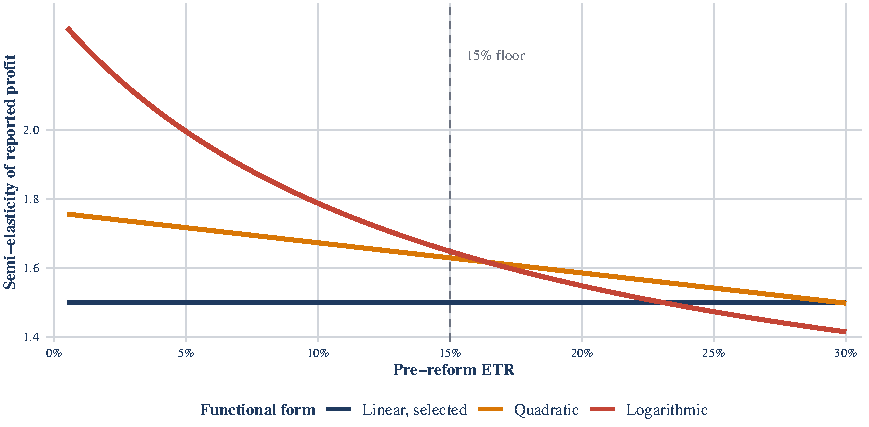
\includegraphics[width=0.82\textwidth]{generated/figures/fig_stage3_semielasticity_estimated.pdf}
\caption[Estimated semi-elasticity schedules.]{Estimated profit-shifting semi-elasticities by pre-reform ETR.}
\label{fig:semi_elasticity_forms}
\end{figure}

\subsection{Allocation and factorial decomposition}\label{sec:results_factorial}

The fourth empirical step turns liability into country revenue and asks which modelling choices drive the scenario spread. The decomposition is run over the full 32-scenario matrix and pooled across EU27 country-years. The result is clear: uncertainty is dominated by measurement of the low-taxed base and by the legal allocation regime, while the behavioural coefficient is statistically visible but quantitatively secondary.

% Generated by code/08_generate_results_tables.R
\begin{table}[H]
\centering
\small
\caption[Pooled factorial decomposition of EU GMT revenue]{Pooled factorial decomposition of EU GMT revenue}
\label{tab:stage4_6_anova_updated}
\begin{tabular}{@{}lrr@{}}
\toprule
Effect & Order & Share (\%) \\
\midrule
ETR measurement & 1 & 51.2 \\
SbS regime & 1 & 36.3 \\
Behavioural response & 1 &  5.0 \\
Substance specification & 1 &  3.5 \\
ETR measurement $\times$ SbS regime & 2 &  1.8 \\
ETR measurement $\times$ Substance specification & 2 &  1.2 \\
ETR measurement $\times$ Behavioural response & 2 &  0.6 \\
SbS regime $\times$ Behavioural response & 2 &  0.2 \\
SBIE rate endpoint & 1 &  0.1 \\
ETR measurement $\times$ SBIE rate endpoint & 2 &  0.0 \\
\bottomrule
\end{tabular}

\vspace{0.5em}
\begin{minipage}{0.96\textwidth}
\footnotesize\raggedright \textit{Notes:} Pooled orthogonal structural variance decomposition across the 32 legally allocated revenue scenarios, EU27 country-years, 2017 to 2022. Source: author's calculations based on \path{data/processed/diagnostics/step7_stage4_6_anova_pooled.csv}.
\end{minipage}
\end{table}



Table \ref{tab:stage4_6_anova_updated} reports the orthogonal factorial decomposition. ETR measurement explains 69.1\% of pooled variance. The SbS regime explains 15.0\%. Behavioural response and substance specification explain 5.1\% and 4.6\%, respectively, while the SBIE rate endpoint explains only 0.1\%. The largest interaction is ETR measurement $\times$ SbS regime at 3.0\%, followed by ETR measurement $\times$ substance specification at 2.1\%. All interactions together explain 6.0\%. The multiplicative pipeline therefore generates interactions, but the main effects already explain the substantive ordering. H2 is supported because ETR measurement is the largest source of scenario variance. H3 is supported because the SbS regime is the second-largest source and changes the legal collection perimeter.

% Generated by code/13_generate_exhibits.R
\begin{table}[H]
\centering
\footnotesize
\setlength{\tabcolsep}{3pt}
\caption[Factorial decomposition of EU GMT revenue]{Factorial decomposition of EU GMT revenue}
\label{tab:stage4_6_factor_decomposition}
\label{tab:stage4_6_shapley_attribution}
\label{tab:stage4_6_main_effects}
\begin{tabular}{@{}l rr rrr r@{}}
\toprule
 & \multicolumn{2}{c}{Variance (\%)} & \multicolumn{4}{c}{Main effects (US\$ bn)} \\
\cmidrule(lr){2-3} \cmidrule(lr){4-7}
Factor & Main & Allocated & Low & High & Effect & Chg (\%) \\
\midrule
ETR measurement & 68.7 & \textbf{71.9} & 223.7 & 485.4 & 261.7 & +117.0 \\
SbS regime & 17.9 & \textbf{20.2} & 419.6 & 289.5 & -130.1 & -31.0 \\
Behavioural response & 3.8 & \textbf{4.2} & 381.1 & 327.9 & -53.2 & -14.0 \\
Substance specification & 2.8 & \textbf{3.5} & 376.8 & 332.2 & -44.6 & -11.8 \\
SBIE rate endpoint & 0.1 & \textbf{0.2} & 348.7 & 360.3 & 11.6 & +3.3 \\
\bottomrule
\end{tabular}

\vspace{0.35em}
\noindent\begin{minipage}{\textwidth}
\footnotesize\raggedright\textit{Notes:} Pooled 32-scenario decomposition, EU27 2017--2023; variance shares are partial $\eta^{2}$.
\end{minipage}
\end{table}


Table \ref{tab:stage4_6_factor_decomposition} reports the Shapley-style allocation alongside cumulative revenue main effects. ETR measurement accounts for 72.0\% of allocated variation; the SbS regime accounts for 16.6\%. The core uncertainty is therefore epistemic measurement uncertainty and institutional legal-regime uncertainty, not the behavioural coefficient. In levels, moving from jurisdiction-average to distributional ETR measurement raises EU revenue from US\$183.7 billion to US\$380.6 billion (+107.3\%). Moving from universal IIR/UTPR collection to the SbS regime lowers revenue from US\$325.9 billion to US\$238.4 billion ($-$26.9\%). The behavioural response and sectoral SBIE with SBTI overlay lower revenue by US\$46.7 billion ($-$15.3\%) and US\$43.6 billion ($-$14.3\%), respectively.

% Generated by code/13_generate_exhibits.R
\begin{table}[H]
\centering
\footnotesize
\setlength{\tabcolsep}{3pt}
\caption[Decomposition stability across higher-measurement windows]{Decomposition stability across higher-measurement windows}
\label{tab:stage46_measurement_sample_decomposition}
\begin{tabular}{@{}L{3.7cm}rrrrrrr@{}}
\toprule
Sample & ETR & SbS & Substance & Behaviour & Interaction & Preferred revenue & Scenario range \\
\midrule
2017–2023 baseline full public panel & 74.7\% & 20.3\% & 0.1\% & 4.7\% & 5.2\% & 367.7 & 196.3--673.4 \\
2019–2023 direct Table IV window & 81.3\% & 15.4\% & 0.1\% & 3.0\% & 5.6\% & 252.8 & 122.2--471.4 \\
2021–2023 Table I and Table IV overlap window & 85.4\% & 12.6\% & 0.0\% & 1.8\% & 5.3\% & 156.1 &  64.0--290.0 \\
2017–2022 comparison window on the updated pipeline & 73.1\% & 21.3\% & 0.2\% & 5.2\% & 5.0\% & 325.8 & 181.6--590.4 \\
\bottomrule
\end{tabular}

\vspace{0.35em}
\noindent\begin{minipage}{\textwidth}
\footnotesize\raggedright\textit{Notes:} ETR, SbS, substance and behaviour columns report Shapley-style allocated shares of the pooled 32-scenario variance. Interaction reports the unallocated ANOVA interaction share before Shapley redistribution. Preferred revenue is cumulative behavioural preferred-core SbS EU revenue in US dollars, billions. Scenario range reports the minimum and maximum cumulative EU revenue across the 32 scenarios in US dollars, billions.
\end{minipage}
\end{table}


As one of the robustness checks, it is checked wheter the full-panel result might be driven by 2017--2018 BSPI backcasting. Table \ref{tab:stage46_measurement_sample_decomposition} reports that this is not the case. ETR measurement accounts for 72.0\% of allocated variation in the full 2017--2022 panel, 80.3\% in the 2019--2022 high-measurement panel, and 84.5\% in the 2021--2022 strict Table IV overlap window.\footnote{This is further analysed in Appendix \ref{app:stage4_allocation}.}. 

\subsection{SbS allocation and country heterogeneity}\label{sec:results_sbs}

The SbS regime changes EU revenue through the collection channel, not through the existence of low-taxed profit. The revenue loss for EU Member States appears in residual IIR and UTPR collection, especially where US-parented low-taxed profit would otherwise have been routed through the UTPR. Table \ref{tab:preferred_channel_updated} shows the preferred-core channel allocation. Under universal collection, cumulative EU revenue is US\$495.8 billion: US\$282.5 billion through QDMTTs, US\$35.8 billion through the IIR and US\$177.5 billion through the UTPR source proxy. Under SbS, QDMTT and IIR revenue remain unchanged in the preferred core, while UTPR revenue falls to US\$38.9 billion. The implied SbS loss is therefore US\$138.6 billion in the preferred-core mechanical scenario. This is why Factor 4 remains the second-largest source of scenario variance, even though the OECD-qualified QDMTT update reduces its share relative to the earlier private-tracker specification.

% Generated by code/08_generate_results_tables.R
{\small
\setlength{\tabcolsep}{4pt}
\begin{longtable}{@{}lrrr@{}}
\caption[Preferred-core revenue by collection channel]{Preferred-core revenue by collection channel}
\label{tab:preferred_channel_updated}\\
\toprule
 & \multicolumn{2}{c}{Revenue (US\$ bn)} & Share (\%) \\
\cmidrule(lr){2-3}
Channel & Universal & SbS & EU total \\
\midrule
\endfirsthead
\multicolumn{4}{c}{\textit{Table~\ref{tab:preferred_channel_updated}---continued}} \\
\toprule
 & \multicolumn{2}{c}{Revenue (US\$ bn)} & Share (\%) \\
\cmidrule(lr){2-3}
Channel & Universal & SbS & EU total \\
\midrule
\endhead
\midrule
\multicolumn{4}{r}{\textit{Continued on next page}}\\
\endfoot
\bottomrule
\endlastfoot
IIR & 35.8 & 35.8 & 7.2 \\
QDMTT & 282.5 & 282.5 & 57.0 \\
UTPR & 177.5 & 38.9 & 35.8 \\
\midrule
Total & 495.8 & 357.2 & 100.0 \\
\end{longtable}
}

\vspace{0.35em}
\noindent\begin{minipage}{\textwidth}
\footnotesize\raggedright\textit{Notes:} Preferred-core scenario; cumulative 2017--2022, US\$ bn.
\end{minipage}


% Generated by code/13_generate_exhibits.R
\begin{table}[H]
\centering
\scriptsize
\setlength{\tabcolsep}{2pt}
\caption[Country revenue uncertainty and fiscal salience]{Country revenue uncertainty and fiscal salience, EU Member States}
\label{tab:country_revenue_diagnostic}
\label{tab:country_spread_updated}
\label{tab:country_fiscal_salience}
\begin{adjustbox}{max width=\textwidth,center}
\begin{tabular}{@{}l rrr r rrrr@{}}
\toprule
 & \multicolumn{3}{c}{Spread} & \multicolumn{5}{c}{Salience} \\
\cmidrule(lr){2-4} \cmidrule(lr){5-9}
Country & Min & Max & Spread & Revenue & Rev./CIT & Spread/CIT & SbS/CIT & QDMTT \\
\midrule
Austria & 4.8 & 8.0 & 3.3 & 4.8 & 5.3\% & 3.6\% & 2.0\% & 71.7\% \\
Belgium & 1.3 & 24.7 & 23.4 & 13.4 & 8.9\% & 15.4\% & 4.2\% & 79.2\% \\
Bulgaria & 1.0 & 2.6 & 1.7 & 1.3 & 9.3\% & 11.9\% & 6.5\% & 66.3\% \\
Croatia & 0.3 & 0.9 & 0.6 & 0.6 & 5.1\% & 5.0\% & 1.0\% & 36.9\% \\
Cyprus & 0.1 & 0.6 & 0.5 & 0.3 & 2.8\% & 4.4\% & 1.5\% & 0.0\% \\
Czechia & 0.7 & 6.0 & 5.2 & 2.4 & 3.3\% & 7.2\% & 3.5\% & 52.1\% \\
Denmark & 3.6 & 13.4 & 9.8 & 8.1 & 9.4\% & 11.3\% & 3.3\% & 79.9\% \\
Finland & 1.2 & 4.9 & 3.7 & 2.6 & 5.1\% & 7.2\% & 2.6\% & 88.7\% \\
France & 2.0 & 65.4 & 63.4 & 24.1 & 5.4\% & 14.1\% & 6.3\% & 54.2\% \\
Germany & 6.1 & 112.4 & 106.3 & 55.3 & 9.3\% & 17.8\% & 5.9\% & 51.0\% \\
Greece & 0.3 & 3.2 & 2.9 & 1.9 & 5.9\% & 9.2\% & 1.9\% & 74.9\% \\
Hungary & 3.3 & 10.1 & 6.8 & 6.6 & 34.6\% & 35.2\% & 8.3\% & 82.6\% \\
Ireland & 36.9 & 66.5 & 29.6 & 37.7 & 32.7\% & 25.7\% & 17.1\% & 76.2\% \\
Italy & 3.1 & 29.0 & 25.9 & 13.4 & 4.2\% & 8.1\% & 3.3\% & 47.7\% \\
Luxembourg & 52.1 & 100.9 & 48.8 & 57.5 & 211.1\% & 179.2\% & 82.8\% & 90.1\% \\
Netherlands & 65.2 & 148.8 & 83.6 & 98.2 & 36.8\% & 31.3\% & 7.6\% & 88.1\% \\
Poland & 0.6 & 13.0 & 12.4 & 4.4 & 4.1\% & 11.5\% & 5.8\% & 45.7\% \\
Portugal & 0.6 & 3.1 & 2.5 & 1.5 & 2.8\% & 4.7\% & 2.1\% & 55.7\% \\
Romania & 1.1 & 6.8 & 5.7 & 3.4 & 8.0\% & 13.4\% & 5.3\% & 27.7\% \\
Slovak Republic & 0.5 & 1.1 & 0.6 & 0.5 & 1.7\% & 2.3\% & 0.0\% & 100.0\% \\
Slovenia & 0.3 & 1.7 & 1.5 & 1.2 & 13.5\% & 17.3\% & 3.0\% & 27.9\% \\
Spain & 4.9 & 37.7 & 32.8 & 20.9 & 8.6\% & 13.6\% & 4.1\% & 58.8\% \\
Sweden & 4.2 & 14.1 & 9.9 & 7.6 & 6.1\% & 7.9\% & 3.2\% & 57.5\% \\
\bottomrule
\end{tabular}
\end{adjustbox}

\vspace{0.35em}
\noindent\begin{minipage}{\textwidth}
\footnotesize\raggedright\textit{Notes:} Cumulative 2017–2023. Spread is the difference between the maximum and minimum across 32 scenarios (US\$ bn). Salience ratios use OECD T\_1200 CIT and the Eurostat equivalent for Cyprus. The table covers states with positive receipts in the preferred behavioural SbS scenario.
\end{minipage}
\end{table}


Table \ref{tab:country_revenue_diagnostic} turns the same revenue matrix into a finance-ministry diagnostic. The spread block reports the 32-scenario range in levels; the salience block scales preferred behavioural SbS revenue and uncertainty by OECD \code{T\_1200} corporate income tax (CIT) revenue. A country with an ETR-measurement-dominated spread needs better information on the within-jurisdiction low-taxed base; a country with an SbS-dominated spread needs to know how much residual Income Inclusion Rule (IIR) and Undertaxed Profits Rule (UTPR) collection disappears once the SbS regime applies. Appendix \ref{app:country_policy} reports the full EU policy matrix and extended fiscal-salience measures. 

Figure \ref{fig:country_salience_uncertainty} puts the fiscal-salience table into a two-dimensional policy map. The horizontal axis measures the preferred behavioural SbS revenue claim relative to cumulative CIT revenue, while the vertical axis measures the full 32-scenario range relative to the same denominator. Countries above the diagonal face more uncertainty than preferred revenue, countries below it have a point estimate larger than the full scenario spread.

\begin{figure}[H]
\centering
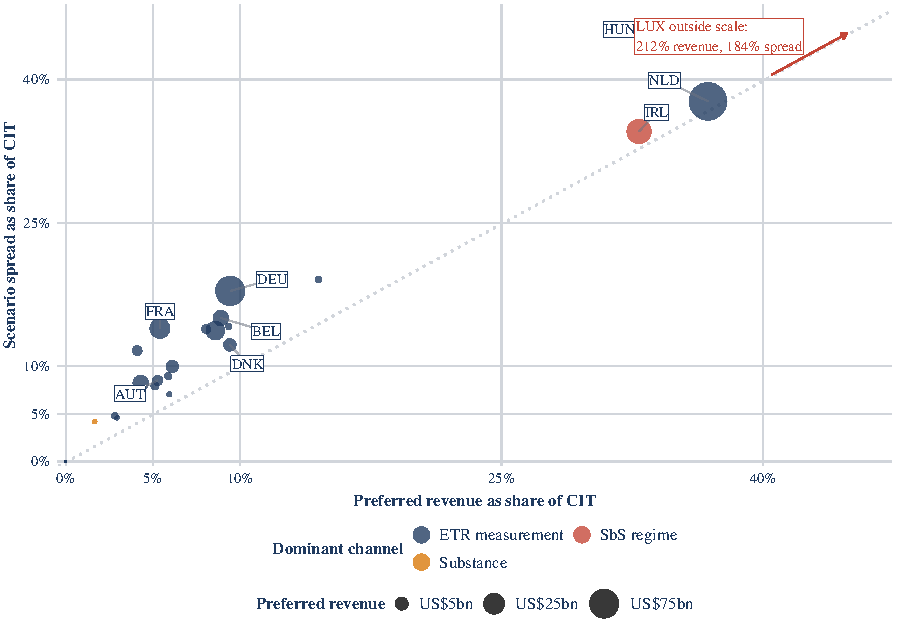
\includegraphics[width=0.96\textwidth]{generated/figures/fig_country_salience_uncertainty.pdf}
\caption[Country fiscal salience and scenario uncertainty.]{Colour reports the largest country-level ANOVA main effect and bubble size reports preferred revenue in current USD. The plotted axes zoom into the 0--45\% range and exclude Luxembourg from the scale. The annotation reports Luxembourg's outside-scale values.}
\label{fig:country_salience_uncertainty}
\end{figure}

Germany is the large fiscal-base case where the revenue number is mainly a measurement statement. Preferred behavioural SbS revenue is US\$44.5 billion, equal to 9.0\% of cumulative CIT revenue. The cumulative scenario spread is US\$79.9 billion, equal to 16.2\% of CIT revenue, and 84.1\% of Germany's country-level scenario variance comes from ETR measurement. The German ministry should therefore treat the point estimate as less informative than the measurement range around it.

The Netherlands is the high-revenue case where a strong QDMTT position reduces the legal-allocation risk. Preferred behavioural SbS revenue is US\$87.1 billion, or 41.4\% of cumulative CIT revenue. The scenario spread is US\$81.0 billion, or 38.5\% of CIT revenue, and ETR measurement explains 72.9\% of the country-level scenario variance. QDMTTs protect 92.2\% of preferred revenue, so the SbS regime extinguishes only 6.0\% of CIT revenue. The practical implication is that Dutch revenue protection is primarily domestic and legal, but the central forecast still rests on the public data's ability to identify low-taxed profit inside average-ETR affiliate cells.

France is a lower-salience large economy with a sizeable residual allocation exposure. Preferred behavioural SbS revenue is US\$20.2 billion, equal to 5.4\% of cumulative CIT revenue. The scenario spread is US\$47.4 billion, or 12.6\% of CIT revenue, and ETR measurement accounts for 72.7\% of the country-level scenario variance. QDMTTs protect 58.5\% of preferred revenue, leaving a larger residual channel than in the Netherlands or Luxembourg. SbS extinguishes 5.0\% of CIT revenue. A French ministry should therefore read the estimate as fiscally smaller than the conduit cases, but legally more exposed to the boundary between protected domestic collection and residual IIR/UTPR collection.

Luxembourg is the salience case where the ratio is too large to read as an ordinary budget forecast. Preferred behavioural SbS revenue is US\$51.7 billion, equal to 225.1\% of cumulative CIT revenue. The scenario spread is US\$41.7 billion, equal to 181.7\% of CIT revenue. Unlike Germany, France and the Netherlands, the dominant uncertainty channel is the SbS regime itself, which explains 58.0\% of country-level scenario variance. QDMTTs protect 92.6\% of preferred revenue, yet SbS extinguishes 77.4\% of CIT revenue. Luxembourg should treat the number as a stress statistic for legal allocation and low-taxed-base measurement, not as a mechanically budgetable cash amount.

Ireland is the case where substance measurement matters more than ETR measurement. Preferred behavioural SbS revenue is US\$27.1 billion, equal to 30.3\% of cumulative CIT revenue. The cumulative scenario spread is US\$26.6 billion, or 29.7\% of CIT revenue. The country-level decomposition attributes 38.1\% of scenario variance to the substance specification, 29.8\% to the SbS regime and 18.1\% to ETR measurement. QDMTTs protect 86.0\% of preferred revenue, while SbS extinguishes 13.7\% of CIT revenue. For Ireland, the policy-relevant uncertainty is the size and sectoral distribution of the Substance-Based Income Exclusion and Substance-Based Tax Incentive (SBTI) capacity, because this determines how much of the low-taxed base survives into top-up tax.

Hungary shows why a smaller Member State belongs in the country section. Preferred behavioural SbS revenue is US\$3.9 billion, much smaller than the five large cases in absolute terms, but it equals 26.8\% of cumulative CIT revenue. The scenario spread is US\$5.8 billion, or 40.2\% of CIT revenue, so the relative uncertainty is larger than in Germany, France and Ireland. ETR measurement is still the largest channel, explaining 54.9\% of country-level scenario variance. QDMTTs protect 88.0\% of preferred revenue and SbS extinguishes 7.3\% of CIT revenue. The lesson is that administrative attention should not follow absolute revenue alone. A small state can face a high-salience forecast when the GMT amount is large relative to its existing CIT base.

% Generated by code/13_generate_exhibits.R
\begin{table}[H]
\centering
\footnotesize
\setlength{\tabcolsep}{3pt}
\caption[PCA of the country typology feature matrix]{PCA of the country typology feature matrix}
\label{tab:country_typology_pca}
\begin{tabular}{@{}lrrL{3.0cm}L{6.0cm}@{}}
\toprule
Component & Variance & Cumulative & Dominant dimension & Largest loadings \\
\midrule
PC1 & 46.9\% & 46.9\% & Fiscal scale & Behavioural effect; Preferred revenue; Revenue per resident; Scenario spread \\
PC2 & 23.4\% & 70.3\% & Legal allocation & Residual IIR/UTPR; QDMTT share; SbS extinguished share; Revenue/CIT \\
PC3 & 12.3\% & 82.6\% & Fiscal scale & Revenue/GDP; Revenue/CIT; Substance effect; High-risk imputation \\
\bottomrule
\end{tabular}

\vspace{0.35em}
\noindent\begin{minipage}{\textwidth}
\footnotesize\raggedright\textit{Notes:} The PCA is run on standardised country-level features. Revenue amounts, scenario spread and per-resident revenue enter in logs; signed main-effect amounts enter as signed log magnitudes. For PCA scaling, median imputation fills undefined channel shares for the four countries with zero assigned receipts.
\end{minipage}
\end{table}


Table \ref{tab:country_typology_pca} uses PCA as a diagnostic before clustering. This matters because a cluster algorithm will always partition the countries, even if the policy variation is essentially one-dimensional. Here the first component explains 48.8\% of the standardised cross-country variation and is dominated by fiscal-scale variables: preferred revenue, scenario spread, per-resident revenue and the behavioural main-effect magnitude, which itself scales with the revenue base. The second component explains 22.6\% and is legal-allocation variation: QDMTT-preserved collection, residual IIR/UTPR exposure and fiscal-salience variables. The third component explains 11.5\% and separates fiscal salience relative to GDP and CIT revenue from absolute scale. The PCA shows that a useful typology must distinguish fiscal scale from legal allocation. 

% Generated by code/08_generate_results_tables.R
{\footnotesize
\setlength{\tabcolsep}{3pt}
\begin{longtable}{@{}L{3.2cm}L{4.8cm}rrrrrrr@{}}
\caption[Policy-facing country typology]{Policy-facing country typology from PCA-informed clustering}
\label{tab:country_typology_clusters}\\
\toprule
Type & Countries & n & Revenue & Revenue/CIT & QDMTT & Residual & SbS extinguished & Imputation risk \\
\midrule
\endfirsthead
\multicolumn{9}{c}{\textit{Table~\ref{tab:country_typology_clusters}---continued}} \\
\toprule
Type & Countries & n & Revenue & Revenue/CIT & QDMTT & Residual & SbS extinguished & Imputation risk \\
\midrule
\endhead
\midrule
\multicolumn{9}{r}{\textit{Continued on next page}}\\
\endfoot
\bottomrule
\endlastfoot
T1: High-salience conduit hubs & LUX &  1 &  51.7 & 225.1\% & 92.6\% &  7.4\% & 25.6\% & 45.6\% \\
T2: QDMTT-protected smaller exposure & AUT, BEL, DNK, FIN, GRC, HUN, IRL, NLD, SVK &  9 & 144.7 &  15.0\% & 86.8\% & 13.2\% & 20.8\% & 39.9\% \\
T3: Residual IIR/UTPR and measurement exposure & BGR, CZE, DEU, ESP, FRA, HRV, ITA, POL, PRT, ROU, SVN, SWE & 12 & 107.3 &   6.1\% & 55.6\% & 44.4\% & 36.0\% & 34.7\% \\
T4: No preferred current exposure & CYP, EST, LTU, LVA, MLT &  5 &   0.0 &   0.0\% &  &  &  & 34.0\% \\
\end{longtable}
}

\vspace{0.35em}
\noindent\begin{minipage}{\textwidth}
\footnotesize\raggedright\textit{Notes:} Four clusters are selected because the jitter stability score is 100.0\%, the smallest cluster contains 1 countries, and the four-cluster solution separates conduit hubs, QDMTT-protected smaller states, residual IIR/UTPR exposure states and zero-current-exposure states. Revenue is preferred behavioural SbS revenue in US dollars, billions. Revenue/CIT uses OECD T\_1200 where available; cluster means ignore missing denominators.
\end{minipage}


Table \ref{tab:country_typology_clusters} reports the resulting country types. The four-cluster solution is chosen because it has 100.0\% jitter stability and gives the most interpretable policy partition. The first type consists only of Luxembourg. It is the high-salience conduit case: preferred behavioural SbS revenue averages 225.1\% of CIT revenue, QDMTTs preserve 92.6\% of preferred revenue, and residual IIR/UTPR exposure is 7.4\%. The second type consists of countries where the QDMTT-protected is but broader than in the private-tracker specification: QDMTTs preserve 86.8\% of preferred revenue and residual IIR/UTPR exposure is 13.2\%. The third type consists of countries with a lower fiscal salience, but residual IIR/UTPR exposure at 44.4\%, so legal allocation remains the relevant policy risk. The fourth type consists of smaller countries, where the preferred behavioural SbS scenario generates no current collector-country revenue. H5 is therefore supported as a classification result: Member States separate into policy profiles defined by fiscal scale, legal allocation and measurement risk, rather than by absolute revenue alone.

\subsection{Hypothesis summary}\label{sec:results_hypotheses}

Table \ref{tab:hypothesis_result_summary} summarises the five hypothesis tests. 

% Generated by code/08_generate_results_tables.R
{\small
\setlength{\tabcolsep}{4pt}
\begin{longtable}{@{}L{1.7cm}L{7.1cm}L{4.8cm}@{}}
\caption[Hypothesis summary]{Hypothesis summary}
\label{tab:hypothesis_result_summary}\\
\toprule
Hypothesis & Main result & Interpretation \\
\midrule
\endfirsthead
\multicolumn{3}{c}{\textit{Table~\ref{tab:hypothesis_result_summary}---continued}} \\
\toprule
Hypothesis & Main result & Interpretation \\
\midrule
\endhead
\midrule
\multicolumn{3}{r}{\textit{Continued on next page}}\\
\endfoot
\bottomrule
\endlastfoot
H1 & The distributional branch raises the EU27 Stage 1 liability rate relative to the jurisdiction-average rule in every year from 2017 to 2022. & Supported. \\
H2 & ETR measurement explains 69.1\% of pooled scenario variance. & Supported. \\
H3 & The SbS regime explains 15.0\% of pooled scenario variance and reduces preferred-core EU revenue by US\$138.6 bn through the UTPR channel. & Supported. SbS is the second-largest variance source and materially changes collection channels. \\
H4 & Tax terms are jointly significant; baseline BIC selects Linear; logarithmic 5\% semi-elasticity is 2.00. & Supported in its cautious form: the panel supports a negative tax-profit relationship, but not a sharply nonlinear lower-tail specification. \\
H5 & PC1 explains 48.8\% of typology variation and the selected four-cluster solution has 100.0\% jitter stability. & Supported. Member States separate into high-salience conduit hubs, QDMTT-protected smaller exposures, residual IIR/UTPR exposure states and zero-current-exposure states. \\
\end{longtable}
}

\vspace{0.35em}
\noindent\begin{minipage}{\textwidth}
\footnotesize\raggedright\textit{Notes:} The table summarises the evidence reported in the Stage 1 to Stage 4.6 diagnostics and the country fiscal-exposure calculations in Section \ref{sec:results_sbs}.
\end{minipage}


\section{Discussion and conclusion}\label{sec:discussion}\label{sec:limitations}

This paper decomposes the revenue of the Global Minimum Tax in the EU. The main result is not that one number is the right number. It is that the spread across plausible public-data estimates is highly structured. Across 32 scenarios, cumulative EU revenue over 2017--2022 ranges from US\$127.7 billion to US\$517.4 billion, and the preferred behavioural SbS scenario gives US\$307.0 billion. The variance decomposition shows that most of this spread is generated before the behavioural coefficient becomes decisive. ETR measurement explains 69.1\% of pooled scenario variance as a raw main effect, or 72.0\% after interaction shares are allocated. The SbS regime explains 15.0\% as a raw main effect, or 16.6\% after interaction allocation.

The substantive interpretation is straightforward. Public CbCR data are informative enough to show that the GMT base is fiscally material, but not precise enough to make the low-taxed base a settled object. Jurisdiction-average ETRs are too coarse for a tax that applies to the low-taxed mass inside a jurisdiction. The distributional branch, anchored where possible on direct Table IV brackets, reveals a deeper top-up gap and therefore a larger liability rate. The direct-observation windows strengthen rather than weaken this result: in 2019--2022 and 2021--2022, where Table IV carries the measurement burden more directly, ETR measurement becomes even more dominant in the decomposition.

The second result is institutional. The January 2026 Side-by-Side Safe Harbour does not make US-parented low-taxed profit disappear. It changes who can collect the top-up. QDMTTs remain operative, while residual IIR and UTPR collection on qualifying US-parented groups is extinguished. The preferred-core channel table makes the mechanism visible. Under universal collection, the EU collects US\$177.5 billion through the UTPR source proxy. Under SbS, this falls to US\$38.9 billion, while QDMTT revenue is unchanged. This is why QDMTT status is not a legal detail in the model. It is the difference between source-country preservation of the claim and exposure to residual collection loss.

The behavioural evidence is useful, but it should not be oversold. The panel estimate supports a negative tax-profit relationship and gives a linear semi-elasticity of 1.50. That is larger than the meta-regression consensus in \citet{heckemeyer2017}, but the public CbCR panel does not support the much sharper lower-tail curvature implied by \citet{dowd2017}. The IV diagnostics are also a warning: simulated EATR and lagged statutory CIT changes are relevant in the first stage, but the reduced forms are too imprecise to replace the fixed-effect estimate with a stronger causal claim. The behavioural response is therefore a disciplined scenario coefficient. It is not the causal centrepiece of the paper.

The country results show why the decomposition is more useful than an EU aggregate. Germany and France are mainly measurement cases: the point estimates matter, but the policy-relevant object is the range created by low-taxed-base measurement. The Netherlands and Luxembourg have much larger fiscal salience, but the interpretation differs. The Dutch result is protected mainly through a strong QDMTT position, while Luxembourg's revenue-to-CIT ratio is so large that the estimate should be read as a stress statistic for legal allocation and measurement exposure, not as a mechanically budgetable cash amount. Ireland is the clearest substance case: its uncertainty is driven more by the sectoral SBIE and SBTI layer than by ETR measurement. Hungary shows that smaller Member States can face high relative exposure even when absolute revenue is modest.

For policymakers, the first implication is that better ETR distribution data would reduce forecast uncertainty more than another marginal refinement of the behavioural semi-elasticity. The most valuable data improvement would be broader, consistent access to bracket-level or micro-level ETR information that identifies the mass below 15\% without forcing a jurisdiction-average collapse. The second implication is legal. Countries that expect low-taxed affiliate exposure have a strong fiscal reason to secure qualified QDMTT status, because the SbS regime makes residual IIR and UTPR collection less reliable. The third implication concerns tax incentives. The SBTI results should be read as capacity rather than take-up: public data reveal where substance-linked incentives could be protected, while actual firm claims under GloBE remain unobserved.

The limitations are material. First, CbCR profit and tax accrued are not GloBE income and covered taxes. GloBE rules adjust financial accounting income for timing differences, permanent differences, losses and covered-tax rules that public CbCR cannot observe \citep{hanlon2023}. This creates measurement error in both the tax base and the ETR. Second, public CbCR is aggregated. The fixed-effect model improves on pure cross-section estimates, but it cannot recover firm-level behavioural heterogeneity or separate book-profit reallocation from real investment responses. Third, the sectoral bridge uses FATS and EUKLEMS to allocate aggregate CbCR quantities across EU host-country sectors. That is appropriate for exposure analysis, but it does not observe sectoral GloBE income or actual SBTI claims. Fourth, the legal allocation flags reflect the OECD Central Record as used in the pipeline. If more regimes become qualified, especially outside the current US SbS case, the allocation result should be rerun.

The uncertainty objects should also remain separate. The 32-scenario spread is not a confidence interval. It is a structural spread across modelling and legal assumptions. The Stage 1 measurement-error interval is a separate residual-propagation diagnostic. The Object C coefficient bound is only a local approximation because the full coefficient bootstrap has not yet been implemented. Collapsing these objects into one interval would make the estimate look more statistically conventional, but it would be less honest. The strongest empirical claim is the ranking of the uncertainty channels, not the precision of any single revenue number.

The thesis therefore answers the research question as follows. In public 2017--2022 OECD CbCR data, EU GMT revenue uncertainty is driven mainly by low-taxed-base measurement and legal allocation under the SbS regime. Substance exclusions and behavioural responses are economically meaningful, but they are second-order relative to these two channels in the current decomposition. A stronger empirical GMT literature should therefore move in two directions: better direct measurement of within-jurisdiction low-taxed profit, and legally precise modelling of QDMTT, IIR, UTPR and safe-harbour status. Without those two improvements, the fiscal debate will continue to confuse behavioural uncertainty with the more basic problem of not knowing, from public data, exactly which profit is below the 15\% floor and which government can collect the tax.

\newpage
\printbibliography[heading=bibintoc]

\newpage
\appendix
\renewcommand{\thesection}{\Alph{section}}
\renewcommand{\theHsection}{appendix.\Alph{section}}
\renewcommand{\theHsubsection}{appendix.\Alph{section}.\arabic{subsection}}
\renewcommand{\theHsubsubsection}{appendix.\Alph{section}.\arabic{subsection}.\arabic{subsubsection}}
\renewcommand{\thetable}{\Alph{section}.\arabic{table}}
\renewcommand{\thefigure}{\Alph{section}.\arabic{figure}}
\renewcommand{\theequation}{\Alph{section}.\arabic{equation}}
\renewcommand{\theHtable}{appendix.\Alph{section}.\arabic{table}}
\renewcommand{\theHfigure}{appendix.\Alph{section}.\arabic{figure}}
\renewcommand{\theHequation}{appendix.\Alph{section}.\arabic{equation}}
\makeatletter
\@addtoreset{table}{section}
\@addtoreset{figure}{section}
\@addtoreset{equation}{section}
\makeatother
\setcounter{table}{0}
\setcounter{figure}{0}
\setcounter{equation}{0}

\section{Data construction and source audit}\label{app:data}

This appendix supports Section \ref{sec:data} Data. 

\subsection{Data sources}\label{app:source_provenance}

All data sources are public. The OECD CbCR tables, OECD statutory CIT rates, OECD forward-looking ETRs and OECD BEPS implementation indicators are collected through the OECD SDMX REST endpoint \url{https://sdmx.oecd.org/public/rest/data}. Eurostat inward FATS is collected through the Eurostat SDMX endpoint \url{https://ec.europa.eu/eurostat/api/dissemination/sdmx/2.1/data}. ILO wage data are collected through the ILO SDMX endpoint \url{https://sdmx.ilo.org/rest/data}. World Bank GDP, population and country-classification data are collected through \url{https://api.worldbank.org/v2/}. BEA U.S. MNE benchmark files are collected from the published BEA file URLs and the BEA API endpoint \url{https://apps.bea.gov/api/data}. EUKLEMS \& INTANProd files are collected from the public download links recorded in \path{code/collect_all_data.py}. Pillar Two legal allocation status is taken from the \url{https://www.oecd.org/content/dam/oecd/en/topics/policy-sub-issues/global-minimum-tax/administrative-guidance-globe-rules-pillar-two-central-record-legislation-transitional-qualified-status.pdf}.

Table \ref{tab:data_sources_units} gives an overview of the data used. 

\begin{table}[H]
\centering
\caption{Data sources, original units, and measurement role}
\label{tab:data_sources_units}
\footnotesize
\begin{tabularx}{\textwidth}{@{}L{2.8cm}L{3.2cm}L{3.2cm}X@{}}
\toprule
Source & Original unit of observation & Main raw variables & Measurement role \\
\midrule
OECD CbCR Table I & Parent jurisdiction $\times$ affiliate jurisdiction $\times$ fiscal year $\times$ profit panel & \code{PROFIT}, \code{PROFIT\_ADJ}, \code{TAX\_ACCRUED}, \code{ASSETS}, \code{EMPLOYEES}, ETR percentiles, business-activity counts & Base bilateral panel, corrected profit, jurisdiction-average ETR, Table I constrained-Beta fit, aggregate SBIE inputs \\
OECD CbCR Table IV & Parent jurisdiction $\times$ affiliate jurisdiction $\times$ fiscal year $\times$ subsidiary-level ETR bracket & Profit, tax, assets, employees and activity counts by ETR bracket, especially \code{RATE\_0-15} & Direct observation of the low-taxed profit bracket and cross-validation of the Table I constrained-Beta fit \\
Eurostat inward FATS & Reporting country $\times$ NACE sector $\times$ controlling country $\times$ year & Employment, turnover, personnel costs, investment and value added & EU host-country sectoral exposure shares for foreign-controlled enterprises, used as a sectoral bridge, not as a Pillar Two population or ETR source \\
EUKLEMS \& INTANProd & Country $\times$ NACE sector $\times$ year & Tangible capital stock, intangible capital stock, value added and labour-account variables & Sectoral tangible-capital shares for decomposing aggregate tangible assets, with intangible-capital measures used only for robustness and interpretation \\
BEA US MNE data & U.S.-parented MOFA country $\times$ industry $\times$ year tables & Property, plant and equipment related series, employment, compensation and value added & External benchmark for U.S.-parented MNE carve-out inputs. Direct replacement requires a further BEA-to-CbCR bridge \\
OECD and ILO wage data & Jurisdiction $\times$ year & Annual or monthly earnings, preferably PPP-adjusted USD & Wage benchmark for the payroll proxy $\hat{W}_{p,j,t}=N_{p,j,t}\bar{w}_{j,t}$ \\
OECD statutory CIT rates & Jurisdiction $\times$ year & Combined central and sub-central statutory CIT rate & Benchmark for CbCR ETR plausibility and instrument in IV diagnostics \\
OECD forward-looking ETRs & Jurisdiction $\times$ year $\times$ tax measure $\times$ investment scenario & EATR, EMTR and capital-allowance measures by fixed/composite project scenario & Simulated tax-code EATR instrument for the behavioural IV diagnostic \\
World Bank macro controls & Jurisdiction $\times$ year & GDP per capita and population & Affiliate-market controls in the Hines--Rice panel regressions \\
BEPS and Pillar Two implementation data & Jurisdiction $\times$ policy instrument $\times$ year & CbCR, CFC, interest-limitation, hybrid-mismatch, OECD-qualified QDMTT, IIR and SbS indicators & Institutional controls and legal allocation variables \\
\bottomrule
\end{tabularx}
\end{table}

\subsection{CbCR panel}\label{app:CbCR}

\subsubsection{Construction of the bilateral CbCR panel}\label{sec:bilateral_panel}

The raw CbCR files are long SDMX tables: each row is a combination of reporting jurisdiction, partner jurisdiction, fiscal year, table type, panel, statistical operation and measure code. The first construction step pivots these rows into a wide parent--affiliate--year panel, with one row per $(p,j,t)$ and one column for each relevant measure. Country-like affiliate observations, regional aggregates and the \code{WXD} aggregate are flagged separately so that world or regional aggregates are not confused with ordinary country-level affiliate cells.

Panel A-I is used for profit-making observations when an ETR denominator is required. Panel A-II and the panel-agnostic aggregate are used only where total real activity is needed, for example for employee counts in the payroll proxy. This separation is important: an ETR is undefined when profit is zero or negative, but employees and tangible assets remain economically meaningful. The measurement panel therefore preserves activity variables for zero-profit cells while excluding or bounding the corresponding ETR observation. 

\subsubsection{Table I: aggregate totals and ETR percentiles}\label{sec:t1_main}

Table I is the starting point for the revenue pipeline. It reports jurisdiction-level financial aggregates for each bilateral parent--affiliate pair, creating a dataset analogous to a trade matrix: each cell represents the total economic activity of all MNEs headquartered in parent jurisdiction $p$ that have constituent entities in affiliate jurisdiction $j$. The financial measures include profit before income tax (\code{PROFIT}), adjusted profit (\code{PROFIT\_ADJ}, available for 2021--2022), income tax accrued (\code{TAX\_ACCRUED}), tangible assets (\code{ASSETS}), employee counts (\code{EMPLOYEES}), and accumulated (retained) earnings (\code{EARNINGS}), among 28 measure codes in total.\footnote{Appendix \ref{app:CbCR} documents the CbCR table structure and the main measure codes used here. Monetary values are denominated in USD. \code{EARNINGS} refers to accumulated (retained) earnings, not current-period payroll. The OECD CbCR template does not contain a payroll variable, so the labour-cost leg of the SBIE must be constructed from \code{EMPLOYEES} and external wage benchmarks (Section \ref{sec:payroll_imputation}).}

Table I is also the only CbCR table that reports moments of the within-jurisdiction ETR distribution, through five bilateral percentiles ($P5, P25, P50, P75, P95$) on the \code{ETR} measure. These percentiles are the empirical input to the distributional measurement developed in Section \ref{sec:distributional}: they are the finest shape information publicly available, and any distributional fit to CbCR data must be anchored on them. Their temporal coverage is tight. The 2017--2020 vintages report no populated percentiles at all. The raw bilateral coverage in 2021--2022 is only 48--51\% on Panel A-I and 59--63\% with the panel-agnostic \code{\_T} fallback. The measurement step does not use single bilateral cells for the fitted distribution. It uses affiliate-year percentiles aggregated across parents. At that level the information loss is much smaller: for 2021 and 2022 together, all 54 EU affiliate-year cells have a complete Panel A-I percentile set, the global sample covers 370 affiliate-years on Panel A-I alone and 410 affiliate-years once an A-I $\rightarrow$ \code{\_T} cascade is allowed, and 239 affiliate-years also carry a usable Table IV validation observation. After requiring positive measurement support and a valid Stage 1 mean anchor, the implemented constrained-Beta object is estimated for 375 affiliate-years, 190 in 2021 and 185 in 2022. Because direct Table IV has priority in the hybrid selector, only the subset not already observed directly enters the selected percentile branch. In the realised bilateral panel this is 820 pair-year cells. Two profit panels are reported: Panel A-I restricts to profit-making entities (positive profit before tax) and is used as the denominator for all ETR calculations. Panel A-II adds loss-makers and is used only where total activity coverage is required. For the EU analysis the affiliate-year coverage of Panel A-I is already complete in 2021--2022, so Panel A-I is the baseline percentile source. The panel-agnostic \code{\_T} series is used only in the non-EU extension and reported as a robustness margin because it mixes profit-makers with loss-makers.

Table I further reports business-activity counts: the number of constituent entities in each bilateral cell classified by primary business activity (holding, IP management, manufacturing, R\&D, finance, and others). The holding-company share (\code{ACT\_HOLDING}/\code{ENTITIES\_COUNT}) is central to the profit-base correction developed in Section \ref{sec:doublecounting}, and the activity composition of the low-tax bracket is an input to the SBIE allocation (Section \ref{sec:sbie_decomp}).

Over the full 2017--2022 panel, Table I spans 58 parent jurisdictions and 240 affiliate jurisdictions. The 2022 vintage contains 54 parent jurisdictions and 221 affiliate jurisdictions. The affiliate dimension includes individual country codes, regional aggregates, and a ``world excluding domestic'' aggregate (\code{WXD}) that captures all foreign affiliate activity.\footnote{Appendix \ref{app:CbCR} documents the full set of aggregate codes. The bilateral structure means that the same affiliate jurisdiction appears in multiple rows, once for each parent jurisdiction that reports MNE activity there.}

\subsubsection{Table IV: subsidiary-level ETR brackets}\label{sec:t4_main}

Table IV partitions all financial variables by 11 ETR brackets at the \emph{subsidiary} level, so the ETR assigned to each observation reflects the individual constituent entity's own jurisdictional effective tax rate, not the MNE group's global average.\footnote{This contrasts with Table III, which assigns ETR brackets at the MNE-group level. \citet{hugger2026} demonstrate that 53.2\% of all low-taxed profit is located in jurisdictions where the \emph{jurisdiction-average} ETR exceeds 15\%, so any aggregation to the jurisdiction mean obscures more than half of the GMT base. Table III's MNE-group aggregation operates on a different axis but raises the same concern. Table IV, which brackets at the subsidiary level, resolves both.} The \code{RATE\_0-15} bracket directly identifies all profit, tangible assets, employees, and tax reported by entities facing an ETR below 15\%: the GMT top-up base without any distributional extrapolation.

Because Table IV observes the quantity that the Table I distributional fit must estimate, it plays two roles in the measurement framework: (i) as the preferred data source inside the hybrid measurement \eqref{eq:lowtax_share} wherever it is observed, and (ii) as the independent benchmark against which the Table I constrained-Beta fit is cross-validated (Section \ref{sec:crossval_tests}). The second role is what makes the approximation error of the five-percentile fit quantifiable rather than assumed.

Table IV covers 49 parent jurisdictions and 154 affiliate jurisdictions over the full 2017--2022 panel. Annual bilateral coverage is narrower. The reduced affiliate coverage relative to Table I reflects OECD confidentiality thresholds: jurisdictions with too few MNE affiliates are suppressed to prevent identification of individual MNE groups. The bilateral structure of Table IV is only available from 2019 onwards. The 2017--2018 vintages report only the \code{WXD} ``world excluding domestic'' aggregate at the subsidiary level. Individual affiliate jurisdictions are not disaggregated. Bilateral parent--affiliate coverage begins in 2019 and contains 41--45 parent jurisdictions and 142--144 affiliate jurisdictions per year in 2019--2022, including all 27 EU Member States continuously over that window. The restriction is not binding for the bilateral low-taxed-profit measurement over 2019--2022: all 27 EU Member States appear in Table IV across that window, and Table IV is therefore the primary source for the EU sample whenever it is observed. The distributional fit on Table I provides the extension to non-EU affiliates where Table IV is unavailable, and the only within-jurisdiction measurement source at all before 2019.

\subsubsection{Tables II, III, V, and VI}\label{sec:other_tables}

The remaining four tables serve supporting roles. Table II reports interquartile means (IQM) of financial variables, the arithmetic mean computed after excluding the bottom and top quartiles of MNE groups within each bilateral pair. This robust central tendency estimator is less sensitive to the extremely large MNE groups that dominate simple averages. It serves as a cross-check on the aggregate totals in Table I for the SBIE computation. Table III disaggregates observations by ETR bracket at the MNE-group level and is therefore less suitable for direct GMT revenue computation than Table IV, but it provides business-activity counts within each ETR range that are informative about the composition of low-taxed activity. Table V reports the size distribution of MNE groups within each parent jurisdiction through seven percentile points (P5 through P95), enabling characterisation of MNE groups near the \EUR750 million threshold. Table VI, the most recently added dimension, breaks down all financial and activity variables by five MNE group revenue size classes for fiscal year 2022 only.

Table \ref{tab:cbcr_raw_architecture} makes the raw CbCR architecture explicit. The central distinction is whether the table is organised by jurisdiction totals, by ETR brackets, or by MNE size. This determines whether the table can measure the GMT base directly, only approximate it, or only validate a supporting assumption.

\begin{table}[H]
\centering
\caption{Original structure of the six public CbCR tables}
\label{tab:cbcr_raw_architecture}
\footnotesize
\begin{tabularx}{\textwidth}{@{}L{1.25cm}L{3.0cm}L{2.6cm}L{3.2cm}X@{}}
\toprule
Table & Raw partition & ETR concept & Main variables used & Role in this thesis \\
\midrule
I & Parent $\times$ affiliate totals, split by profit panel & Jurisdiction-average ETR and five ETR percentiles & Profit, adjusted profit, tax accrued, assets, employees, activity counts, ETR percentiles & Main bilateral panel, average ETR, distributional fit and aggregate SBIE inputs \\
II & Parent $\times$ affiliate interquartile means & No direct bracket, robust central tendency & IQ means of financial and activity variables & Cross-check on whether Table I totals are dominated by very large MNE groups \\
III & ETR brackets at MNE-group level & Group-level ETR bracket & Bracketed financial variables and activity counts & Descriptive composition check, not the preferred GMT base because low-taxed subsidiaries can be hidden inside high-ETR groups \\
IV & ETR brackets at subsidiary level & Subsidiary-level ETR bracket & Bracketed profit, tax, assets, employees and activity counts & Direct measurement of profit below 15\% and validation benchmark for Table I percentiles \\
V & MNE group size percentiles by parent & No ETR bracket & Size-distribution percentiles & Threshold and representativeness context around the \EUR750 million CbCR population \\
VI & MNE group size classes, 2022 only & No ETR bracket & Financial and activity variables by size class & Descriptive size heterogeneity and robustness context \\
\bottomrule
\end{tabularx}
\end{table}

\subsubsection{Profit reconciliation model}\label{sec:profit_correction_reproducibility}

The profit correction is audited separately because it changes the denominator of every later ETR and top-up calculation. The estimand is not a causal effect and not a fitted dividend-flow model. It is the parent-year share of reported domestic UPE profit that should be removed because it represents dividends, participation income or holding-chain profit already counted elsewhere:
\begin{equation}\label{eq:profit_reconciliation_estimand}
\rho_{pt}
=
\frac{\text{double-counted domestic UPE profit}_{pt}}
{\text{reported domestic UPE profit}_{pt}} .
\end{equation}
Public CbCR identifies the single-counted denominator only where OECD adjusted profit is observed. Everywhere else the problem is partially identified measurement error. This is why the baseline in equation \eqref{eq:profit_reconciliation_branch} corrects domestic UPE cells and leaves foreign affiliate cells unchanged. \citet{hugger2026} place the main correction on UPE-jurisdiction profit, while noting that affiliate-to-affiliate dividend chains may remain. Moving those foreign-chain corrections into the preferred branch would require ownership-chain information that public aggregate CbCR does not contain.

The strongest public signal is observed OECD adjusted profit. For any supported group $G$,
\[
\widehat{\rho}^{adj}_{G}
=1-
\frac{\sum_{(p,j,t)\in G}\pi^{adj}_{pjt}}
{\sum_{(p,j,t)\in G}\pi_{pjt}} .
\]
This calculation is internally identified because reported and adjusted profit are observed in the same OECD cell, but support is sparse. In the analytical panel it covers 36 cells and provides direct domestic parent-year or parent-average signals only for the Netherlands and the United Kingdom.

The second layer is external country evidence. The anchor file records the sample scope of each rate so that domestic positive-profit, all-subgroup, IRS CbCR and OECD CbCR evidence are not silently mixed. For the United States, the model uses the year-specific domestic corrections in \citet{garcia-bernardo2022a}: 54\% in 2017, 74\% in 2018 and 42\% in 2019. Those rates are stronger than any public-CbCR-only diagnostic because they reconcile IRS CbCR with Compustat, BEA survey information and imputations for missing firm information. For the Netherlands, Italy, the United Kingdom and Sweden, the anchor file records country-note evidence summarised by \citet{godar2024}. The Netherlands receives a 16\% dividend-component anchor. A broader Dutch participation-result note is retained as validation-only evidence because it is not the same estimand as the dividend-only domestic UPE correction. The residual prior is the 32.4\% median UPE correction reported by \citet{hugger2026}.

The weakest signal is the public domestic-versus-foreign ETR parity diagnostic. For a domestic parent cell in host jurisdiction $j$,
\[
\tau^{D}_{jt}=\frac{C_{jjt}}{\pi_{jjt}},
\qquad
\tau^{F}_{jt}=
\frac{\sum_{p\neq j} C_{pjt}}
{\sum_{p\neq j} \pi_{pjt}},
\]
and the public signal is
\[
\widehat{\rho}^{par}_{jt}
=
\min\left\{0.555,\,
\max\left(0,\,1-\frac{\tau^{D}_{jt}}{\tau^{F}_{jt}}\right)\right\}.
\]
The 55.5\% cap belongs to this public comparison method in \citet{hugger2026}. It is not imposed as an upper bound on the true correction, since the US 2018 reconciliation exceeds it. The diagnostic is filtered to positive domestic profit, non-negative domestic tax, positive foreign-affiliate profit, a positive foreign-affiliate ETR, at least three foreign parent jurisdictions and a minimum foreign-profit mass. It enters with low precision because foreign-owned affiliates are an imperfect control group for domestic UPEs: sector mix, loss histories, tax incentives, holding activity and profit-shifting intensity can all differ.

% Generated by code/13_generate_exhibits.R
\begin{table}[H]
\centering
\footnotesize
\setlength{\tabcolsep}{3pt}
\caption{Evidence hierarchy for the profit-reconciliation model}
\label{tab:profit_correction_evidence_table}
\begin{tabular}{@{}L{2.8cm}L{1.8cm}L{3.4cm}rrrrrr@{}}
\toprule
Evidence & Source & Scope & Rows & Parents & Profit (US\$ bn) & $\rho$ (\%) & Median (\%) & SE \\
\midrule
Fallback prior & hugger2026 & Median upe double counting correction & 318 & 58 & 33,253.7 & 32.4 & 32.4 & 0.160 \\
Macro reconciliation anchor & garcia-bernardo2022a & Domestic positive profit irs cbcr compustat reconciliation &   3 &  1 &  4,409.4 & 57.5 & 54.0 & 0.027 \\
Observed adjusted profit & oecd2025a & Domestic parent year adjusted profit &  10 &  2 &    775.3 & 31.2 & 21.8 & 0.045 \\
Observed adjusted profit, parent average & oecd2025a & Domestic parent average adjusted profit &   5 &  2 &  2,083.3 & 32.2 & 35.2 & 0.075 \\
Official country-note anchor & godar2024 & Domestic positive profit intragroup dividends receivable &   6 &  1 &    812.6 & 49.0 & 49.0 & 0.120 \\
Official country-note anchor & godar2024 & Domestic positive profit median dividend share &   6 &  1 &    316.3 & 28.0 & 28.0 & 0.120 \\
Official country-note anchor & godar2024 & Domestic positive profit tax free dividend sensitivity &   6 &  1 &    303.1 & 52.0 & 52.0 & 0.120 \\
Official country-note anchor & godar2024 & Domestic positive profit dividend component &   6 &  1 &    242.7 & 16.0 & 16.0 & 0.080 \\
Public ETR-parity signal & hugger2026 & Domestic parent year public etr parity & 312 & 54 & 38,355.2 & 14.1 & 22.1 & 0.491 \\
\bottomrule
\end{tabular}

\vspace{0.35em}
\noindent\begin{minipage}{\textwidth}
\footnotesize\raggedright\textit{Notes:} Each row summarises one type of signal entering the parent-year correction model. The fallback prior is the Hugger et al. median UPE correction; the public ETR-parity signal is capped at 55.5\% and enters with low precision.
\end{minipage}
\end{table}


Each evidence row is written as $(p,t,s)$ with signal $\rho_{spt}$, source type $s$, profit weight and source standard error. The implemented model transforms the bounded correction rate to a logit scale,
\[
y_{spt}
=
\log\left(
\frac{\rho_{spt}/u}{1-\rho_{spt}/u}
\right),
\qquad u=0.85 ,
\]
after the public parity signal has already been capped at 0.555. A weighted least-squares prior is then fitted as
\[
y_{spt}
=
\alpha+\gamma_{g(p)}+\delta_t
+\beta_1\log(1+\Pi^D_{pt})
+\beta_2\log(1+A^D_{pt})
+\beta_3\log(1+N^D_{pt})
+\beta_4 H^D_{pt}
+\beta_5 \tau^{stat}_{pt}
+\varepsilon_{spt}.
\]
Here $g(p)$ is the parent group (large UPE jurisdiction, investment hub, zero- or low-tax jurisdiction, or residual), $\Pi^D_{pt}$ is domestic profit mass, $A^D_{pt}$ domestic assets, $N^D_{pt}$ domestic employees, $H^D_{pt}$ the domestic holding-activity share and $\tau^{stat}_{pt}$ the parent statutory rate. Source weights are inverse-variance weights after transforming each signal standard error to the same logit scale. The model prediction is deliberately treated as a prior with a wide residual standard error. Parent-years with direct adjusted-profit evidence or external anchors then combine that prior with the exact signal by inverse-variance weighting. Parent-years without strong evidence shrink toward the group-year prior.

Table \ref{tab:profit_correction_parent_year_top20} reports the largest parent-level corrections. The United States remains anchor-driven in 2017--2019, with partial-pooling extrapolation in 2020--2022. Other large parents combine the \citet{hugger2026} prior with observed adjusted-profit and public-parity support where available. This is the intended interpretation: the model makes the reconciliation evidence-weighted and uncertainty-aware, but it does not claim that public CbCR alone identifies dividend flows.

% Generated by code/13_generate_exhibits.R
\begin{table}[H]
\centering
\footnotesize
\setlength{\tabcolsep}{3pt}
\caption{Largest parent-level profit corrections under the hybrid model}
\label{tab:profit_correction_parent_year_top20}
\begin{tabular}{@{}lrrrrrL{3.0cm}L{2.7cm}@{}}
\toprule
Parent & Years & Profit (US\$ bn) & $\hat{\rho}$ (\%) & Low (\%) & High (\%) & Main source & Support \\
\midrule
USA & 7 & 11,094.1 & 44.5 & 27.3 & 64.0 & macro\_reconciliation; public\_etr\_parity & anchored\_model; parity\_shrinkage \\
CHN & 7 &  7,368.7 & 37.8 & 12.7 & 66.7 & public\_etr\_parity & parity\_shrinkage \\
JPN & 7 &  2,910.0 & 38.6 & 13.1 & 67.3 & public\_etr\_parity & parity\_shrinkage \\
SAU & 6 &  1,748.8 & 30.1 &  9.1 & 60.8 & public\_etr\_parity & parity\_shrinkage \\
CAN & 7 &  1,452.9 & 42.2 & 15.4 & 69.2 & fallback\_prior; public\_etr\_parity & fallback\_prior; parity\_shrinkage \\
DEU & 7 &  1,177.2 & 37.5 & 13.1 & 65.8 & public\_etr\_parity & parity\_shrinkage \\
KOR & 7 &    945.5 & 29.7 &  9.0 & 60.2 & public\_etr\_parity & parity\_shrinkage \\
GBR & 7 &    924.6 & 37.2 & 27.8 & 47.2 & observed\_adjusted\_profit; official\_country\_note & observed\_adjusted \\
FRA & 7 &    758.6 & 34.7 & 11.3 & 64.4 & public\_etr\_parity & parity\_shrinkage \\
BRA & 7 &    730.1 & 35.3 & 11.8 & 64.4 & public\_etr\_parity & parity\_shrinkage \\
AUS & 7 &    681.4 & 27.8 &  8.3 & 58.4 & public\_etr\_parity & parity\_shrinkage \\
IDN & 7 &    560.6 & 38.7 & 13.3 & 67.0 & fallback\_prior; public\_etr\_parity & fallback\_prior; parity\_shrinkage \\
IND & 7 &    523.0 & 30.0 &  9.1 & 60.5 & public\_etr\_parity & parity\_shrinkage \\
CHE & 7 &    433.2 & 21.9 &  6.0 & 52.1 & public\_etr\_parity & parity\_shrinkage \\
NOR & 7 &    396.1 & 32.0 & 10.3 & 61.8 & public\_etr\_parity & parity\_shrinkage \\
ITA & 7 &    382.3 & 31.5 & 14.6 & 53.2 & official\_country\_note; public\_etr\_parity & anchored\_model; parity\_shrinkage \\
MEX & 7 &    367.4 & 33.8 & 11.2 & 62.9 & public\_etr\_parity & parity\_shrinkage \\
MYS & 7 &    357.5 & 30.5 &  9.4 & 60.6 & public\_etr\_parity & parity\_shrinkage \\
HKG & 6 &    348.2 & 25.3 &  7.5 & 55.0 & public\_etr\_parity & parity\_shrinkage \\
SWE & 7 &    325.6 & 43.7 & 25.2 & 62.3 & official\_country\_note; public\_etr\_parity & anchored\_model; parity\_shrinkage \\
\bottomrule
\end{tabular}

\vspace{0.35em}
\noindent\begin{minipage}{\textwidth}
\footnotesize\raggedright\textit{Notes:} Rows are the twenty parent jurisdictions with the largest positive domestic profit over 2017 to 2023. Rates are domestic-profit-weighted averages of parent-year predictions.
\end{minipage}
\end{table}


The validation uses three checks. First, high-credibility signals are held out one source-parent-year at a time and predicted from the remaining evidence. Second, four specifications are compared: uncorrected profit, the earlier static benchmark, parity-only and the hybrid model. This check asks whether the correction moves domestic and foreign ETRs into a more plausible range without mechanically forcing equality. Third, the revenue sensitivity propagates 500 draws of $\rho_{pt}$ through two objects: a pre-SBIE top-up proxy and the preferred behavioural SbS Stage 4.6 panel. The final-revenue propagation keeps distributional low-tax shares, behavioural filters and legal allocation weights fixed, then recomputes the preferred profit denominator and SBIE filter under each draw. It is therefore a conditional profit-correction interval, not a replacement for the main factorial scenario spread.

The domestic-versus-foreign diagnostic is not treated as a loss function. In the realised panel, parity-only gives the smallest profit-weighted absolute domestic-foreign ETR gap, 1.8 percentage points, because it is constructed to close that gap. The hybrid model leaves a larger absolute gap, 11.0 percentage points, and a positive mean gap, 9.6 percentage points. That result is informative: the external anchors imply larger domestic UPE corrections than the public parity proxy would support, especially for the United States. The model therefore prioritises higher-credibility reconciliation evidence over a public-data equality condition that is only weakly identifying.

The appendix also reports a targeted foreign holding-chain sensitivity. This branch is deliberately not part of the preferred estimate. It applies a 10\% residual profit haircut only to foreign affiliate cells in the Netherlands, Luxembourg, Ireland, Switzerland, Singapore, Hong Kong, Bermuda or the Cayman Islands with positive preferred profit, high holding activity, high related-party revenue and low substance relative to profit. The rule flags 43 cells across 16 parent jurisdictions, reducing preferred profit by US\$11.9 billion. Preferred behavioural SbS EU27 revenue falls from US\$303.7 billion to US\$303.4 billion. This small movement is consistent with the baseline choice to leave foreign affiliate cells unchanged unless ownership-chain information is available.

% Generated by code/08_generate_results_tables.R
{\footnotesize
\setlength{\tabcolsep}{3pt}
\begin{longtable}{@{}lrrrrrr@{}}
\caption{Holdout validation for high-credibility profit-correction signals}
\label{tab:profit_correction_validation_holdout}\\
\toprule
Evidence & Rows & Profit (US\$ bn) & Mean error & Mean abs. & Median abs. & Max abs. \\
\midrule
\endfirsthead
\multicolumn{7}{c}{\textit{Table~\ref{tab:profit_correction_validation_holdout}---continued}} \\
\toprule
Evidence & Rows & Profit (US\$ bn) & Mean error & Mean abs. & Median abs. & Max abs. \\
\midrule
\endhead
\midrule
\multicolumn{7}{r}{\textit{Continued on next page}}\\
\endfoot
\bottomrule
\endlastfoot
Macro reconciliation &  3 & 4,409.4 & -15.0 & 15.0 & 13.9 & 28.2 \\
Observed adjusted profit & 10 &   775.3 &   4.8 &  8.4 & 13.7 & 20.1 \\
Official country note & 24 & 1,674.7 &  -4.6 & 11.6 & 11.4 & 18.4 \\
\end{longtable}
}

\vspace{0.35em}
\noindent\begin{minipage}{\textwidth}
\footnotesize\raggedright\textit{Notes:} Each high-credibility signal is held out from the prior fit one source-parent-year at a time and compared with the model prediction. Errors are reported in percentage points of the correction share.
\end{minipage}


% Generated by code/13_generate_exhibits.R
\begin{table}[H]
\centering
\footnotesize
\setlength{\tabcolsep}{3pt}
\caption{Profit-correction uncertainty and preferred-scenario revenue}
\label{tab:profit_correction_revenue_sensitivity}
\begin{adjustbox}{max width=\textwidth,center}
\begin{tabular}{@{}lrrrr@{}}
\toprule
Specification & Positive profit & Global top-up proxy & EU27 top-up proxy & EU27 final SbS \\
\midrule
Uncorrected profit & 55,784.6 & 1,566.5 & 372.5 & 402.4 \\
Low correction & 49,528.3 & 1,323.5 & 316.1 & 379.3 \\
Preferred correction & 41,909.0 & 1,161.3 & 264.2 & 343.8 \\
High correction & 32,699.1 & 1,052.9 & 239.2 & 298.9 \\
500 $\rho_{pt}$ draws & 41,683.9 [40,269.7, 42,916.2] & 1,168.0 [1,147.4, 1,190.5] & 268.0 [261.2, 274.9] & 342.5 [336.6, 348.0] \\
\bottomrule
\end{tabular}
\end{adjustbox}

\vspace{0.35em}
\noindent\begin{minipage}{\textwidth}
\footnotesize\raggedright\textit{Notes:} The top-up proxy is pre-SBIE and pre-allocation: $\max\{0,0.15-\tau\}\pi$ using the drawn corrected denominator. The final SbS column propagates the same parent-year draws through the preferred behavioural Stage 4.6 panel while holding distributional low-tax shares, behavioural filters and legal allocation weights fixed. It is therefore a conditional profit-correction interval, reported separately from the main factorial revenue decomposition.
\end{minipage}
\end{table}


% Generated by code/08_generate_results_tables.R
\begin{table}[H]
\centering
\scriptsize
\caption{Targeted foreign holding-chain profit-correction sensitivity}
\label{tab:profit_correction_foreign_holding_chain}
\begin{adjustbox}{max width=\textwidth,center}
\begin{tabular}{@{}lrrrrr@{}}
\toprule
Object & Cells & Parents & Profit & Global revenue & EU27 final SbS \\
\midrule
Flagged foreign holding-chain cells & 43 & 16 & 118.8 &  &  \\
Preferred domestic-only correction &  &  & 34,840.8 & 892.9 & 303.7 \\
Foreign holding-chain sensitivity &  &  & 34,829.0 & 891.6 & 303.4 \\
Movement relative to preferred &  &  & -11.9 & -1.3 & -0.2 \\
\bottomrule
\end{tabular}
\end{adjustbox}

\vspace{0.5em}
\begin{minipage}{0.96\textwidth}
\footnotesize\raggedright \textit{Notes:} The sensitivity applies a 10\% residual profit haircut only to foreign affiliate cells in the Netherlands, Luxembourg, Ireland, Switzerland, Singapore, Hong Kong, Bermuda or the Cayman Islands with positive preferred profit, high holding activity, high related-party revenue and low substance relative to profit. It is not part of the preferred correction because public aggregate CbCR cannot identify ownership-chain dividends in foreign affiliate cells. Source files: data/processed/diagnostics/step07a\_profit\_correction\_foreign\_holding\_chain.csv; data/processed/diagnostics/step07a\_profit\_correction\_final\_revenue\_points.csv.
\end{minipage}
\end{table}



Table \ref{tab:cleaned_panel_support} records the main coverage and support diagnostics. These figures are descriptive statistics of the constructed analytical panel after country-like affiliate filtering, profit correction flags, wage matching, ETR bounding, and Stage 1 source assignment. The revenue estimates use this cleaned object rather than the full long-form CbCR extract.

\begin{table}[H]
\centering
\caption{Cleaned base panel and implemented measurement support}
\label{tab:cleaned_panel_support}
\footnotesize
\begin{tabularx}{\textwidth}{@{}L{4.7cm}rX@{}}
\toprule
Diagnostic object & Count & Interpretation \\
\midrule
Parent--affiliate--year rows, 2016--2022 & 16{,}915 & Country-like cleaned CbCR panel before restricting to the 2017--2022 main sample \\
Parent jurisdictions & 58 & Reporting ultimate-parent jurisdictions represented in the cleaned panel \\
Affiliate jurisdictions & 228 & Country-like affiliate jurisdictions after excluding regional and world aggregates from ordinary affiliate cells \\
EU27 affiliate rows & 3{,}903 & Cleaned rows where the affiliate jurisdiction is an EU Member State \\
Rows with wage benchmark & 14{,}685 & Rows for which an affiliate-year wage can be matched from the OECD or ILO hierarchy \\
Rows with wage-based payroll proxy & 14{,}610 & Rows with $\hat{W}_{p,j,t}=N_{p,j,t}\bar{w}_{j,t}$ available for SBIE measurement \\
Employee plausibility corrections & 9 & Rows where the employee input is corrected by the implemented plausibility screen \\
Rows with reconciliation profit correction & 344 & Rows where $\pi^{\mathrm{rec}}_{p,j,t}$ differs from reported profit under the preferred reconciliation branch \\
Observed OECD \code{PROFIT\_ADJ} rows & 36 & Direct adjusted-profit observations used in-cell and as local reconciliation evidence rather than as a full backcast model \\
Main analytical pair-year rows, 2017--2022 & 15{,}758 & Pair-year rows that enter Stage 1 branch assignment after excluding the 2016 transition vintage \\
Positive-profit analytical pair-years & 11{,}872 & Pair-year rows with a positive profit base for top-up measurement \\
Behavioural estimation sample & 8{,}971 & Rows used in the preferred Hines--Rice fixed-effect regression after estimation filters \\
Direct Table IV Stage 1 branch & 9{,}395 & Pair-year cells whose distributional low-taxed share is observed directly from subsidiary-level Table IV \\
Constrained-Beta Stage 1 branch & 820 & Pair-year cells whose distributional low-taxed share is supplied by the Table I percentile fit \\
BSPI Stage 1 branch & 3{,}899 & Pair-year cells whose distributional low-taxed share is transported from the 2019--2020 Table IV anchor \\
Average-fallback Stage 1 branch & 1{,}459 & Pair-year cells reduced to the jurisdiction-average fallback after higher-information sources are unavailable \\
No usable Stage 1 source & 185 & Pair-year cells left without a valid source for the distributional branch \\
\bottomrule
\end{tabularx}
\begin{flushleft}
\end{flushleft}
\end{table}

\subsection{Merged bilateral base panel}\label{sec:base_panel_appendix}

This subsection documents the merged bilateral parent--affiliate--year panel produced in Step 2 of the data pipeline. Table \ref{tab:base_panel_coverage_working} reports the coverage of the merged panel by fiscal year and distinguishes the broader behavioural estimation sample from the narrower Stage 1 hybrid sample. Table \ref{tab:base_panel_summary_working} reports unweighted cell-level summary statistics for the behavioural estimation sample. Table \ref{tab:base_panel_flags_working} records the main construction and readiness flags created during the merge. The distributions of the monetary variables are strongly right-skewed, so the median and interquartile range are more informative than the mean alone. Importantly, the CbCR \code{EARNINGS} measure is accumulated earnings rather than payroll, so Step 2 now constructs the SBIE payroll input from employee counts and external wage data instead of treating \code{EARNINGS} as labour cost.

\begin{table}[H]
\centering
\footnotesize
\setlength{\tabcolsep}{3pt}
\caption{Coverage of the merged bilateral base panel by fiscal year}
\label{tab:base_panel_coverage_working}
\begin{tabular}{@{}crrrrrrr@{}}
\toprule
Year & Cells & Par. & Aff. & Pctile (\%) & T-IV $<$15 (\%) & S1 ready & Beh. ready \\
\midrule
2016 & 1,157 & 26 & 184 & 0.0 & 0.0 & 0 & 0 \\
2017 & 2,045 & 38 & 217 & 0.0 & 0.0 & 0 & 1,217 \\
2018 & 2,554 & 46 & 214 & 0.0 & 0.0 & 0 & 1,569 \\
2019 & 2,711 & 50 & 211 & 0.0 & 7.2 & 152 & 1,633 \\
2020 & 2,750 & 52 & 213 & 0.0 & 6.5 & 146 & 1,629 \\
2021 & 2,921 & 52 & 212 & 51.5 & 6.4 & 1,059 & 1,817 \\
2022 & 2,777 & 54 & 209 & 55.0 & 7.2 & 1,081 & 1,707 \\
\midrule
Total & 16,915 & 58 & 228 & 17.9 & 4.5 & 2,438 & 9,572 \\
\bottomrule
\end{tabular}
\vspace{0.35em}
\noindent\begin{minipage}{\textwidth}
\footnotesize\raggedright\textit{Notes:} Country-like affiliates only; 2016 retained for diagnostics only.
\end{minipage}
\end{table}

\begin{table}[H]
\centering
\footnotesize
\setlength{\tabcolsep}{3pt}
\caption{Summary statistics for the behavioural estimation sample}
\label{tab:base_panel_summary_working}
\begin{tabular}{@{}L{5.0cm}rrrrrr@{}}
\toprule
Variable & N & Mean & SD & P25 & Median & P75 \\
\midrule
Corrected profit base (USD bn) & 9,572 & 3.386 & 28.515 & 0.017 & 0.105 & 0.685 \\
Income tax accrued (USD bn) & 9,572 & 0.742 & 8.532 & 0.002 & 0.014 & 0.097 \\
SBIE payroll proxy (USD bn) & 9,572 & 0.771 & 9.546 & 0.004 & 0.025 & 0.137 \\
SBIE tangible assets (USD bn) & 9,572 & 4.206 & 47.295 & 0.014 & 0.108 & 0.707 \\
Employees (thousands) & 9,572 & 16.133 & 151.946 & 0.184 & 1.000 & 4.745 \\
Raw Panel A-I ETR (per cent) & 9,572 & 18.015 & 14.536 & 7.764 & 16.266 & 25.022 \\
Affiliate statutory CIT, headline (per cent) & 8,532 & 20.298 & 8.024 & 15.000 & 20.000 & 25.000 \\
Affiliate GDP per capita (USD thousands) & 9,568 & 26.812 & 26.442 & 6.148 & 15.875 & 44.332 \\
Affiliate population (millions) & 9,572 & 88.308 & 245.249 & 5.857 & 18.933 & 62.378 \\
Holding share, Panel A-I (per cent) & 7,798 & 9.372 & 21.315 & 0.000 & 4.370 & 12.500 \\
\bottomrule
\end{tabular}
\vspace{0.35em}
\noindent\begin{minipage}{\textwidth}
\footnotesize\raggedright\textit{Notes:} Behavioural sample, 2017--2022; unweighted pair-year cells; monetary variables in USD bn.
\end{minipage}
\end{table}

\begin{table}[H]
\centering
\footnotesize
\setlength{\tabcolsep}{3pt}
\caption{Construction and readiness flags in the merged bilateral panel}
\label{tab:base_panel_flags_working}
\begin{tabular}{@{}L{5.5cm}rr@{}}
\toprule
Flag & Cells & Share (\%) \\
\midrule
Total pair-year cells & 16,915 & 100.0 \\
Domestic cells & 318 & 1.9 \\
EU-27 affiliate cells & 3,903 & 23.1 \\
Observed \code{PROFIT\_ADJ} cells & 36 & 0.2 \\
Modelled domestic UPE correction & 308 & 1.8 \\
Rows left unchanged by preferred profit reconciliation & 16,571 & 98.0 \\
Employee counts capped by plausibility rule & 9 & 0.1 \\
Wage benchmark more than 5 years away & 612 & 3.6 \\
Wage-based payroll proxy available & 14,610 & 86.4 \\
Missing wage-based payroll proxy & 2,305 & 13.6 \\
Direct Table IV \code{RATE\_0-15} observation & 760 & 4.5 \\
Complete Panel A-I percentile set & 2,366 & 14.0 \\
\code{\_T} percentile fall-back only & 664 & 3.9 \\
Raw Panel A-I ETR below 0 & 703 & 4.2 \\
Raw Panel A-I ETR above 100\% & 117 & 0.7 \\
Stage 1 hybrid-ready pair-year cells & 2,438 & 14.4 \\
Stage 1 cross-validation pair-year cells & 49 & 0.3 \\
Behavioural estimation sample & 9,572 & 56.6 \\
\bottomrule
\end{tabular}
\vspace{0.35em}
\noindent\begin{minipage}{\textwidth}
\footnotesize\raggedright\textit{Notes:} Shares relative to the full merged panel.
\end{minipage}
\end{table}


\clearpage
\section{Stage 1 low-taxed-base measurement}\label{app:stage1_measurement}

This appendix supports Sections \ref{sec:measurement_framework} and \ref{sec:results_stage1}. The central empirical result depends on whether public CbCR can identify the profit mass below the 15\% threshold, and this appendix documents the bounding rules, distributional fit, BSPI backcast and validation tables that underlie that claim.

\subsection{Measurement framework details}\label{app:measurement_framework}

This section records the construction details behind Section \ref{sec:measurement_framework}: ETR bounding, Table I percentile pooling and conditioning, the bounded distribution fit, BSPI bracket-share transport and the Table I versus Table IV cross-validation.

\subsubsection{ETR construction and bounding}\label{sec:etr_bounding_appendix}

The pair-level ETR proxy is equation \eqref{eq:etr}. It is constructed on positive-profit Panel A-I cells because the tax denominator is meaningful only for profit-making entities. Cells with zero Panel A-I profit are excluded from ETR construction but remain available for employees, tangible assets and the SBIE calculation. In the implemented panel, this removes 82 bilateral cells from ETR construction: 74 are $0/0$ observations and eight report zero profit with positive tax, which implies an infinite raw ETR.

The raw Panel A-I ETR series is then bounded before entering the low-taxed-profit measurement. The base panel contains 703 cells with a negative raw ETR, usually due to tax refunds or loss-offset mechanics on a positive profit denominator. It also contains 117 cells with a raw ETR above 100\%, usually because a small profit denominator amplifies a moderate tax charge. Negative ETRs with absolute value below the loss-offset margin $\zeta=0.05$ are treated as near-zero tax positions and recoded to zero. This affects 300 cells over 2017--2022. Negative ETRs with absolute value above $\zeta$ are excluded from the low-taxed-profit measurement because they are more likely to reflect loss-carryforward artefacts than current-period tax positions. This affects 403 cells. Very high ETRs are capped at the affiliate statutory-rate benchmark plus $\zeta$ where the statutory benchmark is available, and at one otherwise. The affected pair-year remains in the analytical panel, so its profit and activity variables can still enter the SBIE and behavioural stages.

\subsubsection{Percentile conditioning and bounded distribution fit}\label{sec:percentile_fit_appendix}

Table I percentiles are reported at the bilateral parent-affiliate level. The fitted distribution is estimated at the affiliate-year level, so bilateral percentile information is pooled across parents with subgroup-count weights:
\begin{equation}\label{eq:jurisdiction_percentile}
\tau_{j,t}^{(k)}=\frac{\sum_p n_{p,j,t}\tau_{p,j,t}^{(k)}}{\sum_p n_{p,j,t}},\quad k\in\{5,25,50,75,95\},\quad n_{p,j,t}\equiv\code{SUBGROUPS\_COUNT}_{p,j,t}.
\end{equation}
The weighting preserves the interpretation that percentiles are computed over reporting subgroups rather than over parent jurisdictions. When the primary subgroup count is unavailable, the implemented hierarchy uses entity-count fallbacks, with the fallback use reported in Appendix Table \ref{tab:app_stage1_conditioning}.

The pooled percentile vector is conditioned before fitting. Non-monotone percentiles are rearranged into a weakly increasing vector, values outside the admissible unit interval are clipped to $[0,1]$, and boundary cases with a mean anchor at zero or one are treated as degenerate point masses. The fitted object is therefore a bounded approximation to the public percentile information, not a claim that the true affiliate-year ETR distribution is literally Beta distributed.

Let $\bar{\tau}_{j,t}$ denote the jurisdiction-average ETR used as the mean anchor. The percentile set is $\mathcal{K}=\{5,25,50,75,95\}$. The Table I branch fits a mean-constrained Beta distribution on $[0,1]$ by solving:
\begin{equation}\label{eq:beta_fit}
(\hat{a}_{j,t},\hat{b}_{j,t})
=\arg\min_{a,b>0}
\sum_{k\in\mathcal{K}}
\left[
B^{-1}\!\left(\frac{k}{100};a,b\right)-\tau_{j,t}^{(k)}
\right]^2
\quad
\text{s.t.}\quad
\frac{a}{a+b}=\bar{\tau}_{j,t},
\end{equation}
where $B^{-1}(\cdot\,;a,b)$ is the Beta quantile function. The code implements this constrained problem by estimating the precision $a+b$ after fixing the mean. The fitted CDF is:
\begin{equation}\label{eq:beta_cdf}
\tilde{F}_{j,t}(x)=I_x(\hat{a}_{j,t},\hat{b}_{j,t}),\quad x\in[0,1],
\end{equation}
where $I_x(\cdot)$ is the regularised incomplete Beta function. The Table I low-taxed share is then $\tilde{F}_{j,t}(T)$, and the average top-up gap is computed from the fitted first moment below $T$.

\subsubsection{Hybrid estimation bracket-share panel imputation}\label{sec:bspi}

The shape-transport branch of \eqref{eq:lowtax_share} is a direct response to the CbCR's asymmetric temporal coverage. Table IV provides the low-taxed profit share bilaterally for 2019--2022 but is entirely absent at the bilateral level for 2017--2018, and Table I supplies no within-jurisdiction heterogeneity until 2021. A jurisdiction-average collapse across the four pre-2019 fiscal years would mechanically truncate Factor 1 to a single level for more than half of the panel, defeating the factorial comparison that drives the decomposition in Section \ref{sec:decomposition}. BSPI instead borrows the short-run stable component of the Table IV profile: for every EU affiliate $j$ with a positive-profit Table IV observation pooled across parents in the anchor window $A = \{2019, 2020\}$, define the anchor bracket-share vector
\begin{equation}\label{eq:bspi_anchor}
\omega_{j,b}^{\text{anchor}} = \frac{\sum_{t \in A}\pi_{j,t,b}^{\text{IV}}}{\sum_{t \in A}\sum_{b' \in \mathcal{B}^{+}}\pi_{j,t,b'}^{\text{IV}}}, \quad b \in \mathcal{B}^{+},
\end{equation}
where $\mathcal{B}^{+} = \{\code{RATE\_0\text{-}15},\code{RATE\_15},\code{RATE\_20\text{-}30},\code{RATE\_30}\}$ is the positive-profit partition. The BSPI low-taxed share for $t \in I = \{2017, 2018\}$ is the transported bracket mass on $[0, 15\%)$:
\begin{equation}\label{eq:bspi}
\bar{s}_{j}^{<T,\text{BSPI}} = \omega_{j,\code{RATE\_0\text{-}15}}^{\text{anchor}}.
\end{equation}
The transported object is a scalar share rather than a full distribution because the 2019--2022 bilateral Table IV partition is populated essentially only in the two brackets straddling the 15\% floor: \code{RATE\_0-15} and \code{RATE\_15} jointly account for every positive-profit observation in the EU slice of the anchor window, and the higher-rate brackets exist in the partition but carry no bilateral EU data. BSPI's informational content therefore reduces to the low-taxed share, which is precisely what \eqref{eq:lowtax_share} measures and what the SBIE and behavioural steps need as input.

The backcast assumes that the short-run within-affiliate bracket shape is stable enough that the 2019--2020 anchor is informative for 2017--2018. This is not a free assumption and is tested out-of-sample on the 2021--2022 hold-out window. Define the validation profile $\omega_{j,b}^{\text{valid}}$ analogously to \eqref{eq:bspi_anchor} over $V = \{2021, 2022\}$, and compute the per-affiliate total variation distance
\begin{equation}\label{eq:bspi_tv}
\text{TV}_{j}^{\text{BSPI}} = \tfrac{1}{2}\sum_{b \in \mathcal{B}^{+}}\left|\omega_{j,b}^{\text{anchor}} - \omega_{j,b}^{\text{valid}}\right|.
\end{equation}
A small TV distance is the empirical warrant that the bracket shape is approximately time-invariant at the two-year horizon. A large TV distance indicates regime change within the anchor-validation span, for example an ATAD transposition cliff, a statutory-rate reform or a structural break in the affiliate's Table IV footprint. The anchor-validation separation matters: backcasting from 2021 rather than 2019--2020 would span a three- to four-year window across the ATAD I/II entry into force and the TCJA transitional period, whereas a 2019--2020 anchor tested against a 2021--2022 validation keeps the implied backcast within a two-year horizon on either side of the anchor midpoint. Cells above the pre-specified TV threshold are flagged, and the strict variant reassigns those shape-transport observations to the jurisdiction-average fallback. Appendix Section \ref{app:results_stage1} reports the realised TV distribution, the flagged affiliates and the strict-variant support counts.

The design choice is a deliberate departure from a naive pooled-panel imputation. A standard panel-regression imputation (for example, affiliate and year fixed effects with a linear trend) would assume a smoothly time-varying low-taxed share and extrapolate the 2019--2022 trend backward. That approach is dominated here on two grounds. First, the policy-relevant variation in Factor 1 is within-affiliate level, not trend: the semi-elasticity estimation in Section \ref{sec:hines_rice} identifies the response to local ETR changes, and the measured low-taxed share enters multiplicatively with the SBIE shield and the behavioural response. A trend-extrapolation backcast would push low-tax affiliates further away from 15\% in 2017 than in the anchor window, which is the opposite of the economically conservative default. Second, BSPI's validation test is genuinely out-of-sample: the 2021--2022 hold-out is never used to set the backcast, only to gate the assumption. A trend-extrapolation model using the full 2019--2022 sample for fitting would have no analogous hold-out and the ATAD/TCJA structural break would enter the fitted trend rather than being diagnosed by it. BSPI therefore trades some potential efficiency for a transparent falsifiability criterion on the very assumption that keeps the 2017--2018 slice of the factorial meaningful.

\paragraph{Cross-validation tests.}\label{sec:crossval_tests}
Three tests are run on the overlapping sample where Table I percentiles and Table IV brackets are both observed (2021--2022). First, for each $(j, t)$ cell observed in both tables, the low-taxed share from Table I (equation \ref{eq:lowtax_share}) is compared against the Table IV direct share. A Wilcoxon signed-rank test assesses $H_0\colon \text{median}(s^{<T,\text{I}} - s^{<T,\text{IV}}) = 0$. It is preferred over a paired $t$-test because the differences are bounded on $[-1, 1]$ and will not be normally distributed. A systematic positive difference indicates that the constrained-Beta fit overstates the low-taxed share relative to the direct bracket observation. A negative difference indicates that the smooth parametric fit compresses low-taxed mass.

Second, Table IV reports profit volumes in discrete ETR brackets (\code{RATE\_0-15}, \code{RATE\_15}, \code{RATE\_20-30}, \code{RATE\_30}, and the negative-profit categories). Evaluating the Beta CDF \eqref{eq:beta_cdf} at the bracket boundaries produces a predicted profit share for each bracket. For each $(j, t)$ cell the fit is measured by the total variation distance:
\begin{equation}\label{eq:chisq_crossval}
\text{TV}_{j,t} = \tfrac{1}{2}\sum_{b=1}^{B} \left|\hat{\omega}_{j,t,b}^{\text{I}} - \omega_{j,t,b}^{\text{IV}}\right|,
\end{equation}
where $\omega_{j,t,b}^{\text{IV}}$ is the observed profit share in bracket $b$ and $\hat{\omega}_{j,t,b}^{\text{I}}$ is the Table I prediction.\footnote{Total variation is preferred to a chi-square metric because the objects being compared are profit shares (bounded on $[0, 1]$, potentially zero in empty brackets), not multinomial counts with a natural denominator. $\text{TV}_{j,t} \in [0, 1]$ has a direct interpretation as the minimum share of mass that must be reallocated across brackets to match the observed distribution.} High-$\text{TV}_{j,t}$ cells are flagged and their concentration in conduit jurisdictions versus the broader EU indicates whether the approximation error is structural (bimodality-driven) or idiosyncratic.

Third, the overlap is used as a direct calibration test rather than only as a difference table. The direct Table IV low-taxed share is regressed on the fitted Table I low-taxed share and year fixed effects:
\begin{equation}\label{eq:crossval_calibration}
s_{j,t}^{<T,\text{IV}} = a + b\,s_{j,t}^{<T,\text{I}} + \gamma_t + u_{j,t}.
\end{equation}
A slope near one and a high $R^2$ would support using the percentile branch as a main measurement object where Table IV is absent. A low slope or weak fit indicates that the percentile branch is informative but too noisy to discipline the direct Table IV branch. The diagnostics also report the Spearman rank correlation and the 90th percentile absolute error, because policy use depends on whether the fitted branch ranks high-risk jurisdictions correctly and how large the upper-tail error is.

The earlier IQR-error regression is retained only as a secondary diagnostic. For each overlap cell, the code computes two pre-SBIE liability estimates (Table I and IV) holding all other measurement and counterfactual choices constant. The percentage revenue difference is regressed on the within-jurisdiction ETR interquartile range from Table I:
\begin{equation}\label{eq:crossval_regression}
\frac{R_{j,t}^{\text{I}} - R_{j,t}^{\text{IV}}}{R_{j,t}^{\text{IV}}} = \alpha + \delta \cdot \text{IQR}_{j,t}^{\text{ETR}} + \gamma_t + \varepsilon_{j,t},
\end{equation}
where $\gamma_t$ are year fixed effects absorbing vintage changes in CbCR coverage. $\hat{\delta}$ tests whether greater within-jurisdiction ETR dispersion also predicts measurement error in the distributional approach. A significant and stable $\hat{\delta}$ could support a correction factor for non-EU jurisdictions where Table IV is unavailable. The preferred estimator applies no IQR correction. Appendix Section \ref{app:results_stage1} reports the diagnostic evidence behind that decision.

\subsection{Stage 1 validation and measurement diagnostics}\label{app:results_stage1}

These tables are needed to evaluate the main measurement claim. Table \ref{tab:app_stage1_bspi_tv} checks the shape-transport assumption for the pre-2019 years, Table \ref{tab:app_stage1_conditioning} records the percentile-conditioning filters, and Table \ref{tab:app_stage1_crossval} shows the direct Table I versus Table IV validation of the fitted low-taxed share.

% Generated by code/08_generate_results_tables.R
\begin{table}[H]
\centering
\scriptsize
\caption{BSPI total-variation summary}
\label{tab:app_stage1_bspi_tv}
\resizebox{\textwidth}{!}{%
\begin{tabular}{@{}lrrrrrr@{}}
\toprule
Scope & Affiliates & High-TV flagged & Median & P75 & P90 & Maximum \\
\midrule
EU27 & 27 &  3 & 0.093 & 0.196 & 0.358 & 0.665 \\
Non-EU & 90 & 10 & 0.058 & 0.210 & 0.400 & 1.000 \\
\bottomrule
\end{tabular}
}

\vspace{0.5em}
\begin{minipage}{0.96\textwidth}
\footnotesize\raggedright \textit{Notes:} Source: author's calculations based on \path{data/processed/diagnostics/step3_stage1_bspi_tv_summary.csv}.
\end{minipage}
\end{table}


% Generated by code/08_generate_results_tables.R
{\footnotesize
\setlength{\tabcolsep}{3pt}
\begin{longtable}{@{}lrrrrrr@{}}
\caption{Stage 1 percentile and Beta-fit diagnostics}
\label{tab:app_stage1_conditioning}\\
\toprule
Year & Affiliate-years & Non-monotone raw & Out of support & Conditioned & Mean beta fit MAE & Max beta fit error \\
\midrule
\endfirsthead
\multicolumn{7}{c}{\textit{Table~\ref{tab:app_stage1_conditioning}---continued}} \\
\toprule
Year & Affiliate-years & Non-monotone raw & Out of support & Conditioned & Mean beta fit MAE & Max beta fit error \\
\midrule
\endhead
\midrule
\multicolumn{7}{r}{\textit{Continued on next page}}\\
\endfoot
\bottomrule
\endlastfoot
2021 & 190 & 8 &  57 &  62 & 0.115 & 1.000 \\
2022 & 185 & 0 & 108 & 108 & 0.078 & 1.000 \\
\end{longtable}
}

% Generated by code/08_generate_results_tables.R
\begin{table}[H]
\centering
\small
\caption[Beta percentile fit versus Table IV cross-validation]{Beta percentile fit versus Table IV cross-validation}
\label{tab:app_stage1_crossval}
\begin{tabular}{@{}lr@{}}
\toprule
Statistic & Value \\
\midrule
Overlap affiliate-years & 239 \\
Zero-low-share cells in Table IV & 40 \\
Low-taxed share, median gap & 0.153 \\
Low-taxed share, mean absolute error & 0.308 \\
Low-taxed share, p90 absolute error & 0.667 \\
Low-taxed share, Spearman rho & 0.458 \\
Calibration slope, direct on fitted & 0.67 \\
Calibration R-squared & 0.181 \\
Liability rate, median gap & 0.029 \\
Liability rate, mean absolute error & 0.046 \\
Liability rate, p90 absolute error & 0.099 \\
Positive-partition TV, median & 0.546 \\
Positive-partition TV, p90 & 0.949 \\
Low-share Wilcoxon p-value & $7.3 \times 10^{-12}$ \\
\bottomrule
\end{tabular}

\vspace{0.5em}
\begin{minipage}{0.96\textwidth}
\footnotesize\raggedright \textit{Notes:} Differences are Table I constrained-Beta percentile fit minus Table IV direct observation. Calibration regresses the direct Table IV low-taxed share on the fitted Table I low-taxed share and year fixed effects. Source: author's calculations based on \path{data/processed/diagnostics/step3_stage1_crossval_summary.csv}.
\end{minipage}
\end{table}



\clearpage
\section{Stage 2 substance and sectoral exposure}\label{app:stage2_substance}

This appendix supports Sections \ref{sec:SBIE}, \ref{sec:sbti_amplification} and \ref{sec:results_stage2}. The headline 15\% minimum becomes a lower effective floor through the SBIE and SBTI layers, and the sectoral bridge documented here measures that reduction. The bridge is a measurement tool for substance exposure, not an alternative tax dataset.

\subsection{Sectoral decomposition}\label{app:sector}

The sectoral branch is therefore a formal measurement bridge rather than a choice between three competing datasets. CbCR supplies the country-level liability base. FATS and EUKLEMS supply within-country sectoral allocation shares. BEA supplies an external U.S.-parented benchmark for broad-sector validation, not a replacement for either the CbCR base or the EU sectoral bridge. Table \ref{tab:sectoral_bridge_hierarchy} records the hierarchy used in the code. For each country-year and component, the selected sectoral allocation base is normalised to sum to one across the post-2021 FATS leaf sectors. If a sector cell has no usable primary or fallback activity anchor, the cell remains missing for that component and is counted in the bridge-quality diagnostic, rather than being filled with an unsupported sector value.

\begin{table}[H]
\centering
\caption{Sectoral measurement bridge for the SBIE and SBTI layer}
\label{tab:sectoral_bridge_hierarchy}
\footnotesize
\begin{tabularx}{\textwidth}{@{}L{2.5cm}L{3.2cm}L{3.2cm}X@{}}
\toprule
Component & Preferred variable & Fallback rule & Interpretation \\
\midrule
Liability base & CbCR \code{PROFIT}, \code{PROFIT\_ADJ}, \code{TAX\_ACCRUED}, \code{ASSETS}, \code{EMPLOYEES} & None & CbCR remains the only source used to measure top-up liability. Sectoral sources never replace the liability base \\
Payroll share & FATS personnel costs & Employees scaled by observed personnel cost per employee, then turnover scaled by observed personnel-cost-to-turnover ratio & Allocates the wage-based CbCR payroll proxy across EU host-country sectors \\
Asset share & EUKLEMS \code{K\_Tang} tangible capital stock & EUKLEMS stock gap-filled with FATS investment when stock coverage is at least 75\% of FATS turnover, otherwise FATS investment, with activity-scaled suppressed-cell fallback & Allocates the CbCR tangible-asset level across sectors using a stock concept where public coverage is strong enough \\
Profit share & FATS positive gross operating surplus & Positive value added scaled to gross operating surplus, then turnover scaled to gross operating surplus & Allocates the corrected CbCR positive-profit base across sectors for the sectoral effective-floor denominator \\
Validation & BEA employment, compensation, PPE expenditure and total assets & No substitution into the baseline & Tests whether US-parented broad-sector shares are consistent with the FATS/EUKLEMS bridge, especially for the Side-by-Side-relevant US-parent population \\
\bottomrule
\end{tabularx}
\end{table}

A structural break in the FATS data around 2021 complicates the time series. The pre-2021 series uses a single broad activity aggregate and 23 indicators, while the post-2021 series uses 48 NACE-based activity categories and 19 codes. The two halves are not directly comparable. The sectoral estimation therefore uses the post-2021 \code{fats\_activ} data only. Pre-2021 FATS serve as descriptive background. In the 2022 reference matrix the bridge retains 40 non-overlapping FATS leaf sectors for each EU Member State, giving 1{,}080 country-sector cells. The payroll, asset and profit shares each sum to 100\% within every Member State up to numerical precision. Fifteen Member States use EUKLEMS tangible-stock shares for the asset leg, of which seven require within-country investment-based gap-filling for suppressed EUKLEMS cells. Twelve Member States fall back to FATS investment because EUKLEMS tangible-stock coverage does not reach the 75\% turnover threshold. At the level of allocated 2022 sectoral levels, 98.1\% of payroll comes directly from FATS personnel costs, 83.2\% of tangible assets comes from EUKLEMS stock information including gap-filled cells, and 88.2\% of the profit denominator comes from FATS gross operating surplus. Table \ref{tab:fats_raw_structure} records the raw sectoral data structure and its use in the CbCR bridge.

\begin{table}[H]
\centering
\caption{Raw FATS structure and use in the CbCR sectoral bridge}
\label{tab:fats_raw_structure}
\footnotesize
\begin{tabularx}{\textwidth}{@{}L{2.8cm}L{3.2cm}L{3.8cm}X@{}}
\toprule
FATS component & Original partition & Variables used & Measurement implication \\
\midrule
Pre-2021 inward FATS & Reporting economy $\times$ broad activity aggregate $\times$ controlling country $\times$ year & Employment, turnover and personnel-cost indicators in the older \code{fats\_g1b\_08} structure & Used only as descriptive background because the sector taxonomy is not directly comparable with the post-2021 NACE structure \\
Post-2021 inward FATS & Reporting economy $\times$ NACE activity $\times$ controlling country $\times$ year & Personnel costs, employment, turnover, value added and investment in \code{fats\_activ} & EU host-country sectoral shares for foreign-controlled enterprises, payroll-share proxy and sectoral exposure bridge only \\
EUKLEMS \& INTANProd capital module & Country $\times$ NACE activity $\times$ year & Tangible capital stock and intangible capital stock & Preferred public source for sectoral tangible-asset shares. Intangibles enter only as a robustness and interpretation layer \\
FATS-to-CbCR bridge & EU affiliate jurisdiction $\times$ NACE sector $\times$ year & FATS sectoral shares applied to CbCR aggregate levels & Converts CbCR country-level payroll and asset proxies into sectoral SBIE ratios, without treating FATS as a tax dataset \\
\bottomrule
\end{tabularx}
\end{table}

\subsection{SBTI cap and sectoral effective floor}\label{app:sbti_details}

The SBTI Safe Harbour lets qualifying incentives increase covered taxes only up to a substance linked cap. Under Method 1, the cap is:
\begin{equation}\label{eq:substance_cap}
\text{SC}_{p,j,t}^{\text{M1}} = 0.055 \times \max\!\left(\hat{W}_{p,j,t},\; \text{Depr}(A_{p,j,t})\right),
\end{equation}
where $\text{Depr}(A)$ denotes depreciation and depletion of eligible tangible assets. Under Method 2, available for a limited election period, the cap equals 1\% of the carrying value of eligible tangible assets:
\begin{equation}\label{eq:substance_cap_m2}
\text{SC}_{p,j,t}^{\text{M2}} = 0.01 \times A_{p,j,t}.
\end{equation}
Public CbCR observes neither qualifying incentive claims nor depreciation and depletion. Equation \eqref{eq:sbti_capacity} therefore uses the two public-data arms that can be constructed: the Method 1 payroll arm and the Method 2 carrying-value arm. If actual QTI claims were observed, the SBTI-adjusted effective tax rate would be:
\begin{equation}\label{eq:etr_sbti}
\tau_{p,j}^{\text{SBTI}} = \frac{\theta_{p,j} + \min\!\left(\text{QTI}_{p,j},\; \max\!\left(\text{SC}_{p,j}^{\text{M1}},\; \text{SC}_{p,j}^{\text{M2}}\right)\right)}{\pi_{p,j}}.
\end{equation}
The main text does not use \eqref{eq:etr_sbti} as a measured object because the numerator contains unobserved legal claims. It uses $\kappa_{j,q,t}$, the exposure index in equation \eqref{eq:sbti_capacity}.

The sectoral bridge decomposes the aggregate SBIE ratio into sector components. The effective tax floor for sector $q$ in jurisdiction $j$ is:
\begin{equation}\label{eq:floor_sector}
\tau_{j,q}^{\text{floor}} = T - (T-\tau_j)\phi_{j,q}.
\end{equation}
CbCR does not report by sector, so the implementation combines CbCR aggregate levels with sectoral shares from Eurostat FATS and EUKLEMS:
\begin{equation}\label{eq:sbie_sectoral}
\widehat{\text{SBIE}}_{j,q} = \sigma_W \cdot \left(\frac{\text{PersC}_{j,q}^{\text{FATS}}}{\sum_{q'} \text{PersC}_{j,q'}^{\text{FATS}}}\right) \cdot W_j^{\text{CbCR}} + \sigma_A \cdot \left(\frac{\hat{K}_{j,q}}{\sum_{q'} \hat{K}_{j,q'}}\right) \cdot A_j^{\text{CbCR}}.
\end{equation}
Here $\text{PersC}_{j,q}^{\text{FATS}}$ is FATS personnel cost and $\hat{K}_{j,q}$ is the selected tangible-capital allocator from Table \ref{tab:sectoral_bridge_hierarchy}. The effective floor evolves over the SBIE transition period as:
\begin{equation}\label{eq:floor_transition}
\tau_{j,q}^{\text{floor}}(t) = T - (T-\tau_j)\left[\sigma_W(t)\frac{W_{j,q}}{\pi_{j,q}} + \sigma_A(t)\frac{A_{j,q}}{\pi_{j,q}}\right].
\end{equation}
These equations define the sectoral exposure layer. They do not imply that FATS or EUKLEMS observe GloBE income, covered taxes or qualifying incentive claims.

\subsection{Stage 2 implementation diagnostics}\label{app:results_stage2}

These tables are needed only if the reader wants to audit the substance layer in detail. Table \ref{tab:app_stage2_payroll_fallback} records the payroll proxy hierarchy, and Table \ref{tab:app_stage2_asset_sensitivity} checks whether the sectoral asset allocator changes the substantive result.

% Generated by code/08_generate_results_tables.R
{\footnotesize
\setlength{\tabcolsep}{3pt}
\begin{longtable}{@{}lrrrr@{}}
\caption{Stage 2 payroll fallback diagnostics}
\label{tab:app_stage2_payroll_fallback}\\
\toprule
Year & Pair-years & Fallback rows & Positive profit in fallback rows (US\$ bn) & Fallback share of Stage 1 top-up (\%) \\
\midrule
\endfirsthead
\multicolumn{5}{c}{\textit{Table~\ref{tab:app_stage2_payroll_fallback}---continued}} \\
\toprule
Year & Pair-years & Fallback rows & Positive profit in fallback rows (US\$ bn) & Fallback share of Stage 1 top-up (\%) \\
\midrule
\endhead
\midrule
\multicolumn{5}{r}{\textit{Continued on next page}}\\
\endfoot
\bottomrule
\endlastfoot
2017 & 1,554 & 197 & 249.9 & 15.1 \\
2018 & 1,932 & 214 & 178.2 &  9.1 \\
2019 & 2,026 & 203 & 179.7 &  8.6 \\
2020 & 2,011 & 201 & 154.4 &  9.1 \\
2021 & 2,259 & 242 & 268.2 & 10.7 \\
2022 & 2,090 & 219 & 268.8 & 10.7 \\
\end{longtable}
}

% Generated by code/13_generate_exhibits.R
\begin{table}[H]
\centering
\footnotesize
\setlength{\tabcolsep}{3pt}
\caption{Stage 2 sectoral asset sensitivity}
\label{tab:app_stage2_asset_sensitivity}
\begin{tabular}{@{}llrrrr@{}}
\toprule
Rate scenario & Asset sensitivity & Asset scale & Weighted $\phi$ (\%) & Average floor (\%) & Distributional floor (\%) \\
\midrule
Initial & $-25\%$ & 0.75 &  9.4 & 14.9 & 14.2 \\
Initial & Baseline & 1.00 & 10.6 & 14.9 & 14.1 \\
Initial & $+25\%$ & 1.25 & 11.7 & 14.9 & 14.1 \\
Long-run & $-25\%$ & 0.75 &  6.1 & 14.9 & 14.5 \\
Long-run & Baseline & 1.00 &  6.8 & 14.9 & 14.4 \\
Long-run & $+25\%$ & 1.25 &  7.6 & 14.9 & 14.4 \\
\bottomrule
\end{tabular}
\end{table}


\clearpage
\section{Stage 3 behavioural module}\label{app:stage3_behaviour}

This appendix supports Sections \ref{sec:estimation}, \ref{sec:behavioural} and \ref{sec:results_stage3}. The central decomposition is driven by measurement and allocation. The behavioural appendix documents why the preferred semi-elasticity is used as a scenario coefficient rather than as the primary revenue-ranking input.

\subsection{Behavioural functional-form mappings}\label{app:behavioural_details}

The main text uses the BIC-preferred linear mapping. The two rejected nonlinear mappings are reported here because they define the behavioural robustness checks and the scorecard, but they do not drive the central revenue decomposition. Holding real activity fixed, define $G_m(\tau)$ as the counterfactual profit ratio implied by model $m$ when the relevant ETR rises from $\tau$ to the minimum rate $T$. For a generic ETR argument $\tau<T$:
\begin{equation}\label{eq:cf_integral}
\log G_m(\tau) = \int_{\tau}^{T}\frac{\partial \log \pi}{\partial s}\,\mathrm{d}s = -\int_{\tau}^{T}\hat{\varepsilon}_m(s)\,\mathrm{d}s.
\end{equation}
The linear mapping is equation \eqref{eq:cf_linear}. The rejected quadratic mapping is:
\begin{equation}\label{eq:cf_quad}
G_{\text{quad}}(\tau) = \exp\!\left[\hat{\beta}_3(T-\tau) + \hat{\beta}_4(T^2-\tau^2)\right].
\end{equation}
The rejected logarithmic mapping is:
\begin{equation}\label{eq:cf_log}
G_{\text{log}}(\tau) = \exp\!\left[\hat{\beta}_3(T-\tau) + \hat{\beta}_4\left(\log(t_0+T)-\log(t_0+\tau)\right)\right].
\end{equation}
The BIC ranking and the lower-tail support diagnostics in Appendix Section \ref{app:results_stage3} explain why these alternatives are retained as diagnostics and not as the preferred revenue input. Figure \ref{fig:semi_elasticity_forms} reports the corresponding estimated semi-elasticity schedules in the main results.

\subsection{SESH notch diagnostic}\label{app:sesh_details}

The SESH band has the economic structure of a notch: a simplified ETR just below fifteen per cent keeps a jurisdiction in the full GloBE computation, while reaching fifteen per cent deems the top-up tax to be zero. Bunching designs can estimate behavioural responses around such thresholds only when post-policy density is observed near the notch \citep{saez2010,kleven2013,kleven2016}. The present public CbCR panel ends in 2022, before the permanent SESH route can affect reported simplified ETRs. The thesis therefore does not estimate structural bunching.

The implemented SESH term is a pre-reform exposure diagnostic and an upper-bound revenue sensitivity. The code bins jurisdiction-year average ETRs around the fifteen per cent threshold and records how much profit lies close enough to plausibly reach the safe harbour under covered-tax and income management. This diagnostic is useful for a later post-reform paper, but it is not evidence that firms have already bunched. For this reason, the main text includes only the operational liability filter in equation \eqref{eq:regime}.

\subsection{Stage 3 estimation diagnostics}\label{app:results_stage3}

These tables document the econometric support for the behavioural module. They are needed when assessing whether the fixed-effect semi-elasticity is credible. They are not needed to follow the arithmetic of the revenue pipeline.

% Generated by code/08_generate_results_tables.R
{\small
\setlength{\tabcolsep}{4pt}
\begin{longtable}{@{}lrrrrrr@{}}
\caption[Stage 3 model comparison]{Stage 3 model comparison}
\label{tab:stage3_model_comparison}\\
\toprule
Model & $N$ & Pairs & Within $R^2$ & BIC rank & $\Delta$BIC & Tax Wald $p$, two-way \\
\midrule
\endfirsthead
\multicolumn{7}{c}{\textit{Table~\ref{tab:stage3_model_comparison}---continued}} \\
\toprule
Model & $N$ & Pairs & Within $R^2$ & BIC rank & $\Delta$BIC & Tax Wald $p$, two-way \\
\midrule
\endhead
\midrule
\multicolumn{7}{r}{\textit{Continued on next page}}\\
\endfoot
\bottomrule
\endlastfoot
Linear & 8,971 & 1,936 & 0.0339 & 1 & 0.00 & $1.5 \times 10^{-6}$ \\
Logarithmic & 8,971 & 1,936 & 0.0343 & 2 & 5.40 & $1.2 \times 10^{-6}$ \\
Quadratic & 8,971 & 1,936 & 0.0341 & 3 & 7.54 & $1.5 \times 10^{-6}$ \\
\end{longtable}
}

\vspace{0.35em}
\noindent\begin{minipage}{\textwidth}
\footnotesize\raggedright\textit{Notes:} Two-way fixed-effect Hines-Rice models. The BIC ranking is the model-selection rule used in the current pipeline.
\end{minipage}

% Generated by code/08_generate_results_tables.R
\begin{table}[H]
\centering
\small
\caption[Stage 3 fixed-effect regression estimates]{Stage 3 fixed-effect regression estimates. Dependent variable is log profit. Coefficients are reported with two-way parent-and-affiliate clustered standard errors in parentheses.}
\label{tab:stage3_regression_table}
\begin{tabular}{@{}lccc@{}}
\toprule
 & Linear & Quadratic & Logarithmic \\
\midrule
ETR & -1.506*** (0.273) & -1.767* (0.911) & -0.948 (0.955) \\
ETR squared &  &  0.439 (1.269) &  \\
Log shifted ETR &  &  & -0.209 (0.398) \\
Log tangible assets & -0.017 (0.015) & -0.017 (0.015) & -0.017 (0.015) \\
Log payroll proxy &  0.023 (0.034) &  0.023 (0.034) &  0.023 (0.034) \\
Log GDP per capita &  0.675*** (0.109) &  0.676*** (0.109) &  0.676*** (0.108) \\
Log population &  0.728 (0.911) &  0.755 (0.907) &  0.770 (0.912) \\
\midrule
$N$ & 8,971 & 8,971 & 8,971 \\
Parent-affiliate pairs & 1,936 & 1,936 & 1,936 \\
Affiliate clusters &   151 &   151 &   151 \\
Within $R^2$ &     0.0340 &     0.0341 &     0.0344 \\
BIC rank &     1 &     3 &     2 \\
$\Delta$BIC &     0.00 &     7.56 &     5.26 \\
Joint tax-term $p$ & $1.6 \times 10^{-6}$ & $1.6 \times 10^{-6}$ & $1.4 \times 10^{-6}$ \\
\bottomrule
\end{tabular}

\vspace{0.5em}
\begin{minipage}{0.96\textwidth}
\footnotesize\raggedright \textit{Notes:} All models include parent-affiliate pair fixed effects and year fixed effects. $^{*}p<0.10$, $^{**}p<0.05$, $^{***}p<0.01$. Source files: data/processed/diagnostics/step5\_stage3\_coefficients.csv; data/processed/diagnostics/step5\_stage3\_model\_comparison.csv.
\end{minipage}
\end{table}


% Generated by code/08_generate_results_tables.R
\begin{table}[H]
\centering
\scriptsize
\caption[Statutory-CIT instrument diagnostics]{Statutory-CIT instrument diagnostics}
\label{tab:stage3_iv_diagnostics}
\resizebox{\textwidth}{!}{%
\begin{tabular}{@{}llrrrrr@{}}
\toprule
Diagnostic & Dependent variable & Coefficient & Weak-IV $F$ & $p$-value & $N$ & Within $R^2$ \\
\midrule
First stage: CbCR ETR & CbCR ETR &  0.256*** (0.057) & 20.34 & $4.5 \times 10^{-5}$ & 8,033 & 0.0038 \\
Reduced form: log profit & Log profit & -0.296 (0.410) & 20.34 & 0.474 & 8,033 & 0.0057 \\
FE-2SLS: log profit & Log profit & -1.157 (1.581) & 20.34 & 0.468 & 8,033 & 0.0348 \\
\bottomrule
\end{tabular}
}

\vspace{0.5em}
\begin{minipage}{0.96\textwidth}
\footnotesize\raggedright \textit{Notes:} The table reports a fixed-effect first stage, reduced form and linear FE-2SLS robustness estimate. The excluded instrument is the one-year lagged statutory CIT rate of the affiliate jurisdiction. The weak-instrument statistic is the parent-and-affiliate clustered first-stage F-statistic for the excluded instrument. The 2SLS row is not used for the nonlinear counterfactual because one excluded instrument identifies only the linear ETR coefficient. Source: author's calculations based on \path{data/processed/diagnostics/step5_stage3_tax_endogeneity_diagnostics.csv}.
\end{minipage}
\end{table}


% Generated by code/13_generate_exhibits.R
\begin{table}[H]
\centering
\footnotesize
\setlength{\tabcolsep}{3pt}
\caption[Econometric diagnostics for the behavioural stage]{Econometric diagnostics for the behavioural stage}
\label{tab:stage3_econometric_scorecard}
\begin{tabular}{@{}L{3.2cm}L{5.4cm}L{6.2cm}@{}}
\toprule
Diagnostic & Result & Reading \\
\midrule
Preferred fixed-effect model & Linear; $N=$10,611; pairs $=$ 2,031; within $R^2=$ 0.0315; $\Delta$BIC log $=$ 2.53, quadratic $=$ 5.81. & The tax-profit relationship is visible after pair and year fixed effects, but the extra nonlinear parameters add little baseline fit. \\
Joint tax-term tests & Linear $F=$ 36.37, $p=$ $2.4 \times 10^{-7}$; quadratic $p=$ $2.2 \times 10^{-7}$; logarithmic $p=$ $2.0 \times 10^{-7}$. & The tax terms are jointly relevant under two-way clustered inference. \\
Non-nested nonlinear tests & Vuong $p=$ 0.276; Clarke $p=$ $5.3 \times 10^{-62}$; J-test $p=$ 0.163 and 0.280. & The logarithmic form is stronger than the quadratic form, but these tests do not overturn the linear BIC choice. \\
Tax-code IV diagnostics & First-stage $F=$ 10.81 for simulated EATR and 2.09 for lagged statutory CIT; 2SLS $p=$ 0.156 and 0.921. & External tax-code variation is relevant, yet the reduced-form profit response is too imprecise to replace the fixed-effect estimate. \\
Low-ETR support & Below 5\% ETR: 17.1\% of rows and 9.3\% of profit; 5--15\% ETR: 27.0\% of rows. & The GMT-relevant tail is present, while extreme lower-tail curvature remains weakly supported. \\
Sample robustness & Linear is BIC-preferred in 3 of 4 reported samples; the balanced-pair sample selects logarithmic. & The baseline coefficient survives standard sample cuts, with curvature becoming stronger only in the balanced subset. \\
Jurisdiction influence & Leave-one semi-elasticity range 1.37--1.56; preferred model stable in 26 of 27 cases; revenue change -25.5\% to 4.0\%. & The behavioural coefficient is stable; final revenue remains exposed to high-leverage jurisdictions. \\
\bottomrule
\end{tabular}

\vspace{0.35em}
\noindent\begin{minipage}{\textwidth}
\footnotesize\raggedright\textit{Notes:} The table compacts the formal diagnostics that support the Stage 3 behavioural counterfactual. It is generated from the same fixed-effect, IV, model-selection, tail-support and influence outputs used in the appendix.
\end{minipage}
\end{table}

% Generated by code/08_generate_results_tables.R
{\small
\setlength{\tabcolsep}{4pt}
\begin{longtable}{@{}lrrrrr@{}}
\caption[Stage 3 semi-elasticity schedule]{Stage 3 semi-elasticity schedule}
\label{tab:stage3_semielasticity}\\
\toprule
Model & ETR & Semi-elasticity & SE & $p$-value & Reallocation share \\
\midrule
\endfirsthead
\multicolumn{6}{c}{\textit{Table~\ref{tab:stage3_semielasticity}---continued}} \\
\toprule
Model & ETR & Semi-elasticity & SE & $p$-value & Reallocation share \\
\midrule
\endhead
\midrule
\multicolumn{6}{r}{\textit{Continued on next page}}\\
\endfoot
\bottomrule
\endlastfoot
Linear &  5\% & 1.50 & 0.27 & $1.5 \times 10^{-6}$ & 13.9\% \\
Linear & 10\% & 1.50 & 0.27 & $1.5 \times 10^{-6}$ &  7.2\% \\
Quadratic &  5\% & 1.72 & 0.79 & 0.035 & 15.4\% \\
Quadratic & 10\% & 1.67 & 0.67 & 0.016 &  7.9\% \\
Logarithmic &  5\% & 2.00 & 1.13 & 0.083 & 16.5\% \\
Logarithmic & 10\% & 1.79 & 0.74 & 0.019 &  8.2\% \\
\end{longtable}
}

\vspace{0.35em}
\noindent\begin{minipage}{\textwidth}
\footnotesize\raggedright\textit{Notes:} Standard errors are two-way clustered by parent and affiliate. Reallocation share is the implied reduction when the effective rate is raised to 15 per cent.
\end{minipage}

% Generated by code/08_generate_results_tables.R
{\footnotesize
\setlength{\tabcolsep}{3pt}
\begin{longtable}{@{}lrrrrrrr@{}}
\caption{Stage 3 estimation-sample diagnostics}
\label{tab:app_stage3_sample_summary}\\
\toprule
Sample & Rows & Pairs & Affiliates & Parents & Median pair-years & Median ETR (\%) & Stale-wage rows \\
\midrule
\endfirsthead
\multicolumn{8}{c}{\textit{Table~\ref{tab:app_stage3_sample_summary}---continued}} \\
\toprule
Sample & Rows & Pairs & Affiliates & Parents & Median pair-years & Median ETR (\%) & Stale-wage rows \\
\midrule
\endhead
\midrule
\multicolumn{8}{r}{\textit{Continued on next page}}\\
\endfoot
\bottomrule
\endlastfoot
Balanced pairs & 4,770 &   795 & 114 & 33 & 6.0 & 17.2 & 113 \\
Baseline & 8,971 & 1,936 & 151 & 47 & 6.0 & 16.6 & 279 \\
Exclude 2020 2021 & 5,443 & 1,657 & 138 & 43 & 4.0 & 16.6 & 148 \\
Exclude stale wages & 8,669 & 1,879 & 147 & 47 & 6.0 & 17.0 &   0 \\
\end{longtable}
}

% Generated by code/08_generate_results_tables.R
{\footnotesize
\setlength{\tabcolsep}{3pt}
\begin{longtable}{@{}llrrrr@{}}
\caption{Stage 3 tax coefficients}
\label{tab:app_stage3_tax_coefficients}\\
\toprule
Model & Term & Estimate & SE & $p$-value & Within $R^2$ \\
\midrule
\endfirsthead
\multicolumn{6}{c}{\textit{Table~\ref{tab:app_stage3_tax_coefficients}---continued}} \\
\toprule
Model & Term & Estimate & SE & $p$-value & Within $R^2$ \\
\midrule
\endhead
\midrule
\multicolumn{6}{r}{\textit{Continued on next page}}\\
\endfoot
\bottomrule
\endlastfoot
Linear & ETR & -1.500 & 0.272 & $1.5 \times 10^{-6}$ & 0.0339 \\
Quadratic & ETR & -1.761 & 0.909 & 0.059 & 0.0341 \\
Quadratic & ETR squared &  0.438 & 1.262 & 0.730 & 0.0341 \\
Logarithmic & ETR & -0.943 & 0.973 & 0.338 & 0.0343 \\
Logarithmic & Log shifted ETR & -0.214 & 0.415 & 0.609 & 0.0343 \\
\end{longtable}
}

\vspace{0.35em}
\noindent\begin{minipage}{\textwidth}
\footnotesize\raggedright\textit{Notes:} Inference is two-way clustered by parent and affiliate.
\end{minipage}

% Generated by code/08_generate_results_tables.R
{\footnotesize
\setlength{\tabcolsep}{3pt}
\begin{longtable}{@{}lllrrL{4.2cm}@{}}
\caption{Stage 3 non-nested specification tests}
\label{tab:app_stage3_specification_tests}\\
\toprule
Test & Model A & Model B & Statistic & $p$-value & Interpretation \\
\midrule
\endfirsthead
\multicolumn{6}{c}{\textit{Table~\ref{tab:app_stage3_specification_tests}---continued}} \\
\toprule
Test & Model A & Model B & Statistic & $p$-value & Interpretation \\
\midrule
\endhead
\midrule
\multicolumn{6}{r}{\textit{Continued on next page}}\\
\endfoot
\bottomrule
\endlastfoot
vuong gaussian observation ll & Logarithmic & Quadratic &     0.868 & 0.386 & logarithmic favoured \\
clarke sign & Logarithmic & Quadratic & 5,221.000 & $1.5 \times 10^{-54}$ & logarithmic favoured \\
davidson mackinnon j & Quadratic & Logarithmic &     1.244 & 0.215 & alternative fitted value in quadratic \\
davidson mackinnon j & Logarithmic & Quadratic &    -1.037 & 0.302 & alternative fitted value in logarithmic \\
\end{longtable}
}

% Generated by code/08_generate_results_tables.R
{\footnotesize
\setlength{\tabcolsep}{3pt}
\begin{longtable}{@{}llrrrrr@{}}
\caption{Stage 3 joint tax-term Wald tests}
\label{tab:app_stage3_wald_tests}\\
\toprule
Model & Tax terms & df num. & df den. & $F$-statistic & $p$-value & Within $R^2$ \\
\midrule
\endfirsthead
\multicolumn{7}{c}{\textit{Table~\ref{tab:app_stage3_wald_tests}---continued}} \\
\toprule
Model & Tax terms & df num. & df den. & $F$-statistic & $p$-value & Within $R^2$ \\
\midrule
\endhead
\midrule
\multicolumn{7}{r}{\textit{Continued on next page}}\\
\endfoot
\bottomrule
\endlastfoot
Linear & tau & 1 & 46 & 30.47 & $1.5 \times 10^{-6}$ & 0.0339 \\
Quadratic & tau + tau\_sq & 2 & 46 & 18.21 & $1.5 \times 10^{-6}$ & 0.0341 \\
Logarithmic & tau + log\_tau & 2 & 46 & 18.55 & $1.2 \times 10^{-6}$ & 0.0343 \\
\end{longtable}
}

\vspace{0.35em}
\noindent\begin{minipage}{\textwidth}
\footnotesize\raggedright\textit{Notes:} Inference is two-way clustered by parent and affiliate.
\end{minipage}

% Generated by code/13_generate_exhibits.R
\begin{table}[H]
\centering
\footnotesize
\setlength{\tabcolsep}{3pt}
\caption{Stage 3 model-selection robustness}
\label{tab:app_stage3_robustness}
\begin{tabular}{@{}llrrrrr@{}}
\toprule
Sample & Model & $N$ & Within $R^2$ & BIC rank & $\Delta$BIC & Tax Wald $p$ \\
\midrule
Balanced pairs & Logarithmic &  5,110 & 0.0946 & 1 &   0.00 & $4.2 \times 10^{-5}$ \\
Balanced pairs & Quadratic &  5,110 & 0.0879 & 2 &  38.02 & $1.3 \times 10^{-5}$ \\
Balanced pairs & Linear &  5,110 & 0.0739 & 3 & 106.96 & $8.7 \times 10^{-6}$ \\
Baseline & Linear & 10,611 & 0.0315 & 1 &   0.00 & $2.4 \times 10^{-7}$ \\
Baseline & Logarithmic & 10,611 & 0.0321 & 2 &   2.53 & $2.0 \times 10^{-7}$ \\
Baseline & Quadratic & 10,611 & 0.0318 & 3 &   5.81 & $2.2 \times 10^{-7}$ \\
Exclude 2020 2021 & Linear &  7,164 & 0.0385 & 1 &   0.00 & $2.1 \times 10^{-6}$ \\
Exclude 2020 2021 & Logarithmic &  7,164 & 0.0392 & 2 &   3.16 & $7.2 \times 10^{-6}$ \\
Exclude 2020 2021 & Quadratic &  7,164 & 0.0392 & 3 &   3.79 & $8.1 \times 10^{-6}$ \\
Exclude stale wages & Linear & 10,206 & 0.0316 & 1 &   0.00 & $1.6 \times 10^{-6}$ \\
Exclude stale wages & Logarithmic & 10,206 & 0.0321 & 2 &   4.40 & $1.9 \times 10^{-6}$ \\
Exclude stale wages & Quadratic & 10,206 & 0.0318 & 3 &   6.95 & $2.1 \times 10^{-6}$ \\
\bottomrule
\end{tabular}
\end{table}

% Generated by code/08_generate_results_tables.R
\begin{table}[H]
\centering
\scriptsize
\caption{Stage 3 lower-tail ETR support}
\label{tab:app_stage3_etr_tail_support}
\resizebox{\textwidth}{!}{%
\begin{tabular}{@{}lrrrrrrr@{}}
\toprule
ETR band & Rows & Row share (\%) & Profit share (\%) & Pairs & Affiliates & Parents & Median ETR (\%) \\
\midrule
Below 5\% & 1,569 & 17.5 & 10.4 &   735 & 129 & 38 &  1.1 \\
5\% to 15\% & 2,506 & 27.9 & 34.4 & 1,113 & 132 & 45 & 10.3 \\
15\% and above & 4,896 & 54.6 & 55.2 & 1,508 & 143 & 42 & 24.2 \\
\bottomrule
\end{tabular}
}

\vspace{0.5em}
\begin{minipage}{0.96\textwidth}
\footnotesize\raggedright \textit{Notes:} The table reports the support for the behavioural ETR regressor after winsorisation in the baseline fixed-effect estimation sample. An illustrative tail-balanced design that forces the below-5\% band to 50\% of weighted rows would use a tail multiplier of 2.86 and a non-tail multiplier of 0.61 with effective N equal to 5,178 and a design effect of 1.73. This is a support diagnostic, not an inverse-probability-weighted estimator. 
\end{minipage}
\end{table}


% Generated by code/08_generate_results_tables.R
\begin{table}[H]
\centering
\footnotesize
\setlength{\tabcolsep}{2pt}
\caption{Stage 3 applied behavioural response by year}
\label{tab:app_stage3_behaviour_by_year}
\begin{adjustbox}{max width=\textwidth,center}
\begin{tabular}{@{}lrrrrrr@{}}
\toprule
Year & Aff.-years & EU27 aff.-years & Mean $\beta$ (\%) & Profit-wtd $\beta$ (\%) & Bunching aff.-years & Realloc. aff.-years \\
\midrule
2017 & 201 & 27 & 10.1 & 12.7 & 3 & 141 \\
2018 & 198 & 27 &  9.7 & 12.5 & 6 & 135 \\
2019 & 188 & 27 & 10.1 & 12.4 & 1 & 135 \\
2020 & 191 & 27 &  9.5 & 11.6 & 5 & 126 \\
2021 & 194 & 27 & 10.9 & 11.6 & 4 & 143 \\
2022 & 188 & 27 & 11.4 & 12.4 & 7 & 157 \\
\bottomrule
\end{tabular}
\end{adjustbox}
\end{table}

% Generated by code/08_generate_results_tables.R
\begin{table}[H]
\centering
\scriptsize
\caption{Stage 3 behavioural identification design}
\label{tab:app_stage3_behavioural_design}
\resizebox{\textwidth}{!}{%
\begin{tabular}{@{}L{2.7cm}L{4.1cm}L{3.7cm}L{5.1cm}@{}}
\toprule
Component & Baseline treatment & Identification status & Data for structural extension \\
\midrule
Reallocation share & Estimated from the CbCR fixed-effect semi-elasticity and applied only where a legal collection channel remains active. & Identified as a reduced-form profit response, not as a structural destination-choice parameter. & Private firm-level CbCR or unconsolidated affiliate accounts observed around tax shocks, with group identifiers and affiliate balance sheets. \\
Low etr nonlinearity & Quadratic and logarithmic semi-elasticity specifications are estimated, but the preferred estimator is still chosen by BIC. A lower-tail support diagnostic reports below-5 per cent observations and an illustrative tail-balanced reweighting design. & The current public CbCR panel identifies tax responsiveness more credibly than it identifies the curvature of the response at the extreme lower ETR tail. Tail upweighting is not treated as IPW because the public data do not observe a sampling or treatment-selection probability for below-5 per cent ETR cells. & MNE-jurisdiction microdata or a quasi-experimental tax shock with dense support below 5 per cent, plus a defensible model for the probability that an observation enters the lower tail. \\
Reallocation cap & No discretionary cap is imposed; the response is bounded only to the unit interval. & A cap below one is not identified from public aggregate CbCR data. & Observed post-reform relocation shares from private CbCR or tax-return microdata. \\
Sesh notch bunching & Implemented as an upper-bound liability filter inside the simplified ETR band below 15 per cent. & Not structurally identified from the 2017-2022 public CbCR panel, which is pre-reform and does not observe a post-SESH density spike. & Post-SESH MNE-jurisdiction microdata with simplified ETRs, safe-harbour elections and enough support around the 15 per cent threshold to estimate missing and excess mass. \\
Channel split & Diagnostic only. The short-run split uses the Heckemeyer-Overesch meta-regression distinction between transfer-pricing or licensing and financial-planning channels. & The channel split does not affect top-up tax revenue in the legal allocation matrix. & Royalty, licence, service-fee, interest, intra-group debt and IP ownership data by MNE group and affiliate. \\
Substance relocation & Set to zero in the short-run behavioural response because payroll and tangible assets are held fixed in the SBIE calculation. & Real activity relocation is a longer-run margin and cannot be separated from book-profit shifting in aggregate CbCR. & Firm-level employment, payroll, tangible-asset and investment responses around anti-avoidance or GMT implementation shocks. \\
Destination matrix & Uses the Garcia-Bernardo and Jansky activity-weighted formula as a profit-conservation diagnostic. & Public CbCR does not observe origin-destination flows of shifted profit, so PPML or conditional logit would describe profit stocks rather than identify counterfactual relocation flows. & Origin-destination royalty, interest, service-fee or profit-flow data, plus destination choice sets, statutory and effective tax rates, withholding taxes, treaty links and anti-avoidance rules. \\
\bottomrule
\end{tabular}
}

\vspace{0.5em}
\begin{minipage}{0.96\textwidth}
\footnotesize\raggedright \textit{Notes:} Source: author's calculations based on \path{data/processed/diagnostics/step5_stage3_behavioural_identification_design.csv}.
\end{minipage}
\end{table}



\subsection{Uncertainty quantification}\label{sec:beta_uncertainty}

The headline revenue number hides the same three uncertainty objects defined in Section \ref{sec:two_uncertainties}. The reallocation factor $\hat{\beta}_{j,t}^{e,m}$ is a nonlinear transformation of estimated tax coefficients, the selected functional form, the Stage 1 top-up rate and the SESH bandwidth. These channels should not be collapsed into one statistic. Following the standard distinction between aleatoric and epistemic uncertainty \citep{hullermeier2021}, the thesis treats coefficient sampling error as aleatoric and the choice of measurement or policy scenario as epistemic or institutional.

Object C enters through $(\hat{\beta}_3,\hat{\beta}_4)$ in the Hines--Rice model. The current pipeline reports this uncertainty through cluster-robust standard errors, joint tax-term tests and the interim coefficient-propagation bound in Section \ref{sec:results_stage3}. A full propagation exercise would draw the relevant clusters with replacement, re-estimate the semi-elasticity coefficients, recompute the selected behavioural mapping in equation \eqref{eq:cf_linear}, and rerun the revenue allocation. That object would be a confidence interval around a single scenario, not an additional factorial factor. The factorial contrast between ``mechanical'' and ``behavioural'' scenarios is therefore not itself aleatoric. It is the revenue consequence of applying the point-estimated behavioural coefficient rather than setting it to zero.

Object A covers the ETR measurement factor, the aggregate-versus-sectoral substance factor, the SBIE rate endpoint, the SbS regime factor and their interactions in the full factorial design. These are modelling and institutional uncertainties, not sampling errors that vanish with a larger CbCR panel. They arise because public data do not reveal the true within-jurisdiction low-taxed profit distribution, the true sectoral composition of the GloBE substance shield, or the final legal perimeter of safe-harbour implementation. Object B is narrower: it keeps the scenario fixed and propagates the Stage 1 ETR measurement-error residuals, while separately flagging the BSPI affiliates whose anchor-to-validation shape is unstable.

The BIC and Vuong test identify a preferred specification, but preference is not uniqueness. The quadratic and logarithmic specifications predict semi-elasticities that rise sharply below the lowest ETR observed in the estimation sample. A \emph{no-extrapolation} variant would cap $\hat{\varepsilon}(\tau)$ at $\hat{\varepsilon}(\tau_{\min})$ for all $\tau < \tau_{\min}$, where $\tau_{\min}$ is the 5th percentile of observed affiliate-level ETRs. The gap between the main and no-extrapolation estimates quantifies dependence on out-of-sample functional-form assumptions. In the present results, this is reported as a sensitivity margin rather than as the preferred estimand.

\clearpage
\section{Stage 4 allocation and decomposition diagnostics}\label{app:stage4_allocation}

This appendix supports Sections \ref{sec:sbs}, \ref{sec:decomposition}, \ref{sec:results_factorial} and \ref{sec:results_sbs}. The SbS regime determines which governments can collect top-up tax, and legal allocation is the second-largest source of scenario variance. The tables below document allocation totals, US-parented exposure affected by SbS, decomposition-window robustness checks and jurisdiction-influence diagnostics.

\subsection{Allocation diagnostics}\label{app:results_stage45}

% Generated by code/13_generate_exhibits.R
\begin{table}[H]
\centering
\footnotesize
\setlength{\tabcolsep}{3pt}
\caption{Stage 4.5 allocation summary}
\label{tab:app_stage45_summary}
\begin{tabular}{@{}lr@{}}
\toprule
Metric & Value \\
\midrule
Factorial scenarios &              32 \\
EU27 country-year revenue rows &           6,048 \\
Global allocation conservation, maximum absolute gap &               0.001 \\
UTPR parent-year weight rows &           6,587 \\
UTPR fallback weight rows &             308 \\
H4 mean delta (SbS minus Universal) &  -0.522 \\
H4 median delta (SbS minus Universal) &  -0.116 \\
H4 Wilcoxon p-value & $< 10^{-300}$ \\
Max IIR ambiguous parent share &               0.000 \\
Max UTPR ambiguous collector share &               0.000 \\
EU27 revenue minimum scenario (US\$ bn) & 144.277 \\
EU27 revenue maximum scenario (US\$ bn) & 584.879 \\
\bottomrule
\end{tabular}
\end{table}

% Generated by code/08_generate_results_tables.R
\begin{table}[H]
\centering
\scriptsize
\caption{Selected source-country SbS exposure}
\label{tab:app_stage45_sbs_source_exposure}
\resizebox{\textwidth}{!}{%
\begin{tabular}{@{}lrrrr@{}}
\toprule
Source country & QDMTT & Total top-up (US\$ bn) & US-parented top-up (US\$ bn) & Extinguished (US\$ bn) \\
\midrule
Netherlands & Yes & 92.8 & 37.7 &  0.0 \\
Ireland & Yes & 24.7 & 19.9 &  0.0 \\
Luxembourg & No & 56.9 & 28.8 & 28.8 \\
Germany & Yes & 30.4 &  4.0 &  0.0 \\
France & No & 14.1 &  1.3 &  1.3 \\
\bottomrule
\end{tabular}
}

\vspace{0.5em}
\begin{minipage}{0.96\textwidth}
\footnotesize\raggedright \textit{Notes:} Preferred-core source exposure before final collector-country allocation. Source: author's calculations based on \path{data/processed/diagnostics/step6_stage4_5_sbs_source_exposure.csv}.
\end{minipage}
\end{table}


% Generated by code/08_generate_results_tables.R
{\footnotesize
\setlength{\tabcolsep}{3pt}
\begin{longtable}{@{}lrrrrr@{}}
\caption{Country-level Side-by-Side allocation regression}
\label{tab:app_stage45_h4_regression}\\
\toprule
Term & Estimate & SE & Statistic & $p$-value & $R^2$ \\
\midrule
\endfirsthead
\multicolumn{6}{c}{\textit{Table~\ref{tab:app_stage45_h4_regression}---continued}} \\
\toprule
Term & Estimate & SE & Statistic & $p$-value & $R^2$ \\
\midrule
\endhead
\midrule
\multicolumn{6}{r}{\textit{Continued on next page}}\\
\endfoot
\bottomrule
\endlastfoot
(Intercept) &  -14,315,895.3097 & 249,946,420.0203 & -0.06 & 0.955 & 0.748 \\
source qdmttTRUE & -143,531,412.6042 & 243,727,083.0627 & -0.59 & 0.562 & 0.748 \\
source us parented topup share &   50,221,063.0944 & 537,012,362.5037 &  0.09 & 0.926 & 0.748 \\
preferred scenario revenue &           -0.0228 &           0.0033 & -6.92 & $4.6 \times 10^{-7}$ & 0.748 \\
\end{longtable}
}


\subsection{Decomposition and influence diagnostics}\label{app:results_stage46}

% Generated by code/13_generate_exhibits.R
\begin{table}[H]
\centering
\scriptsize
\setlength{\tabcolsep}{2pt}
\caption[Decomposition-window robustness diagnostics]{Decomposition-window robustness diagnostics}
\label{tab:app_stage46_measurement_sample_decomposition}
\begin{adjustbox}{max width=\textwidth,center}
\begin{tabular}{@{}L{3.7cm}rrrrrrrr@{}}
\toprule
Sample & ETR main & SbS main & Subst. main & Behav. main & Interaction & Direct T. IV & Hi-risk branch & Overlap \\
\midrule
2017–2023 baseline full public panel & 72.2\% & 18.1\% & 0.1\% & 4.3\% & 5.2\% & 67.9\% & 32.3\% & 68 \\
2019–2023 direct Table IV window & 78.5\% & 13.0\% & 0.1\% & 2.7\% & 5.6\% & 97.3\% &  2.9\% & 68 \\
2021–2023 Table I and Table IV overlap window & 82.8\% & 10.2\% & 0.0\% & 1.6\% & 5.3\% & 97.2\% &  3.2\% & 68 \\
2017–2022 comparison window on the updated pipeline & 70.6\% & 19.2\% & 0.1\% & 4.9\% & 5.0\% & 63.0\% & 37.1\% & 43 \\
\bottomrule
\end{tabular}
\end{adjustbox}

\vspace{0.35em}
\noindent\begin{minipage}{\textwidth}
\footnotesize\raggedright\textit{Notes:} Main columns report raw main-effect shares of the pooled 32-scenario ANOVA. Interaction is the aggregate share of all non-main effects. Direct Table IV and high-risk branch columns report EU affiliate low-taxed profit shares in the Stage 1 distributional branch. Overlap cells are affiliate-year validation cells with both percentile and direct Table IV support.
\end{minipage}
\end{table}

% Generated by code/08_generate_results_tables.R
\begin{table}[H]
\centering
\scriptsize
\caption{Highest EU revenue scenarios}
\label{tab:app_stage46_top_scenarios}
\resizebox{\textwidth}{!}{%
\begin{tabular}{@{}llllllr@{}}
\toprule
Scenario & ETR & Substance & Rates & Regime & Behaviour & EU revenue (US\$ bn) \\
\midrule
x10100 & Distributional & Aggregate SBIE & Long-run & Universal & Mechanical & 546.3 \\
x10000 & Distributional & Aggregate SBIE & Initial & Universal & Mechanical & 524.0 \\
x11100 & Distributional & Sectoral SBIE with SBTI & Long-run & Universal & Mechanical & 495.3 \\
x11000 & Distributional & Sectoral SBIE with SBTI & Initial & Universal & Mechanical & 480.0 \\
x10101 & Distributional & Aggregate SBIE & Long-run & Universal & Behavioural & 408.1 \\
x10001 & Distributional & Aggregate SBIE & Initial & Universal & Behavioural & 391.2 \\
x11101 & Distributional & Sectoral SBIE with SBTI & Long-run & Universal & Behavioural & 370.3 \\
x10110 & Distributional & Aggregate SBIE & Long-run & SbS & Mechanical & 369.7 \\
\bottomrule
\end{tabular}
}

\vspace{0.5em}
\begin{minipage}{0.96\textwidth}
\footnotesize\raggedright \textit{Notes:} Source: author's calculations based on \path{data/processed/diagnostics/step7_stage4_6_scenario_summary.csv}.
\end{minipage}
\end{table}


% Generated by code/13_generate_exhibits.R
\begin{table}[H]
\centering
\footnotesize
\setlength{\tabcolsep}{3pt}
\caption{Largest country-level main effects}
\label{tab:app_stage46_country_anova}
\begin{tabular}{@{}llr@{}}
\toprule
Country & Effect & Share (\%) \\
\midrule
France & ETR measurement & 69.7 \\
France & SbS regime & 22.3 \\
France & Behavioural response &  0.7 \\
Germany & ETR measurement & 83.3 \\
Germany & SbS regime & 11.8 \\
Germany & Behavioural response &  0.8 \\
Ireland & SbS regime & 44.4 \\
Ireland & ETR measurement & 35.8 \\
Ireland & Behavioural response &  4.7 \\
Luxembourg & SbS regime & 60.4 \\
Luxembourg & ETR measurement & 17.3 \\
Luxembourg & Behavioural response & 14.4 \\
Netherlands & ETR measurement & 79.2 \\
Netherlands & Behavioural response &  9.5 \\
Netherlands & SbS regime &  6.8 \\
\bottomrule
\end{tabular}
\end{table}

% Generated by code/13_generate_exhibits.R
\begin{table}[H]
\centering
\scriptsize
\setlength{\tabcolsep}{2pt}
\caption{Leave-one-jurisdiction influence robustness}
\label{tab:app_jurisdiction_influence_summary}
\begin{adjustbox}{max width=\textwidth,center}
\begin{tabular}{@{}lL{2.5cm}lrrrrl@{}}
\toprule
Drop & Jurisdiction & Reason & Profit share (\%) & Semi-elast. & Stage 1 chg (pp) & Pref. rev. chg (\%) & Largest eff. \\
\midrule
Parent & United States (USA) & high leverage, named & 30.3 & 1.48 & -0.59 & -25.5 & ETR measurement \\
Affiliate & Netherlands (NLD) & named &  2.8 & 1.41 & -0.15 & -25.0 & ETR measurement \\
Affiliate & Luxembourg (LUX) & named &  1.3 & 1.46 & -0.11 & -14.3 & ETR measurement \\
Parent & Germany (DEU) & high leverage, named &  5.1 & 1.46 &  0.01 & -14.0 & ETR measurement \\
Affiliate & Germany (DEU) & high leverage, named &  2.9 & 1.46 &  0.03 &  -9.9 & ETR measurement \\
Affiliate & Ireland (IRL) & named &  2.2 & 1.45 &  0.01 &  -9.2 & ETR measurement \\
Parent & China (CHN) & high leverage & 13.6 & 1.37 &  0.33 &  -8.9 & ETR measurement \\
Parent & France (FRA) & high leverage, named &  3.0 & 1.47 &  0.02 &  -6.9 & ETR measurement \\
Affiliate & China (CHN) & high leverage & 16.7 & 1.42 &  0.65 &  -6.9 & ETR measurement \\
Affiliate & United States (USA) & high leverage, named & 19.0 & 1.45 & -0.04 &  -6.3 & ETR measurement \\
Parent & Netherlands (NLD) & named &  1.4 & 1.47 & -0.02 &  -5.4 & ETR measurement \\
Parent & Luxembourg (LUX) & named &  1.3 & 1.56 & -0.02 &  -5.0 & ETR measurement \\
Affiliate & France (FRA) & named &  1.9 & 1.47 &  0.04 &  -4.3 & ETR measurement \\
Affiliate & United Kingdom (GBR) & high leverage &  5.2 & 1.44 & -0.07 &   4.0 & ETR measurement \\
\bottomrule
\end{tabular}
\end{adjustbox}

\vspace{0.35em}
\noindent\begin{minipage}{\textwidth}
\footnotesize\raggedright\textit{Notes:} Rows are sorted by the absolute change in preferred-core behavioural SbS EU revenue. The preferred core uses distributional ETR measurement, aggregate SBIE and initial carve-out rates.
\end{minipage}
\end{table}

% Generated by code/13_generate_exhibits.R
\begin{table}[H]
\centering
\footnotesize
\setlength{\tabcolsep}{2pt}
\caption{Influence range for core decomposition effects}
\label{tab:app_jurisdiction_influence_decomposition}
\begin{adjustbox}{max width=\textwidth,center}
\begin{tabular}{@{}lrrrrrr@{}}
\toprule
Effect & Baseline (\%) & Min (\%) & Max (\%) & Baseline effect & Min effect & Max effect \\
\midrule
ETR measurement & 68.7 & 61.2 & 90.1 &  261.7 &  168.4 & 296.5 \\
SbS regime & 17.9 &  0.0 & 24.3 & -130.1 & -179.6 &   0.0 \\
Behavioural response &  3.8 &  2.7 &  7.1 &  -53.2 &  -59.5 & -30.3 \\
\bottomrule
\end{tabular}
\end{adjustbox}

\vspace{0.35em}
\noindent\begin{minipage}{\textwidth}
\footnotesize\raggedright\textit{Notes:} Variance-decomposition shares and main effects are recomputed after each leave-one-parent and leave-one-affiliate omission. Main effects are cumulative over 2017 to 2023 and expressed in US dollars, billions.
\end{minipage}
\end{table}


\clearpage
\section{Country-level policy appendix}\label{app:country_policy}

This appendix supports Section \ref{sec:results_sbs}. Readers interested in finance-ministry interpretation will find the full country-level detail here. The tables are not needed to follow the main decomposition, but they are essential for country-specific claims about QDMTT protection, residual IIR/UTPR exposure, SbS extinguishment, fiscal salience and typology membership.

\subsection{Full country policy matrix}\label{app:country_policy_matrix}

% Generated by code/08_generate_results_tables.R
\begin{table}[H]
\centering
\scriptsize
\caption{Country policy matrix, full EU sample}
\label{tab:app_country_policy_matrix}
\begin{adjustbox}{max width=\textwidth,center}
\begin{tabular}{@{}lrrrrlrrl@{}}
\toprule
Country & Preferred revenue & Revenue/CIT & Spread & Spread/CIT & Dominant channel & QDMTT protected & SbS extinguished & Imputed measurement \\
\midrule
Austria &  3.8 &   5.2\% &  3.0 &   4.1\% & ETR measurement (93.7\%) &  76.2\% & 19.8\% & Limited (20.2\%) \\
Belgium & 11.9 &   9.5\% & 17.6 &  13.9\% & ETR measurement (82.3\%) &  82.3\% & 21.6\% & Moderate (33.8\%) \\
Bulgaria &  1.0 &   9.3\% &  1.3 &  12.0\% & ETR measurement (52.9\%) &  69.5\% & 34.1\% & Limited (17.5\%) \\
Croatia &  0.4 &   4.8\% &  0.4 &   4.6\% & ETR measurement (73.8\%) &  44.7\% & 13.2\% & Heavy (100.0\%) \\
Cyprus &  0.0 &  &  0.0 &  & None &  &  & Limited (13.9\%) \\
Czechia &  1.8 &   3.1\% &  3.7 &   6.3\% & ETR measurement (69.0\%) &  57.6\% & 44.8\% & Moderate (33.4\%) \\
Denmark &  8.1 &  11.3\% &  9.4 &  13.0\% & ETR measurement (77.1\%) &  84.4\% & 17.0\% & Moderate (29.6\%) \\
Estonia &  0.0 &   0.0\% &  0.0 &   0.0\% & None &  &  & Limited (12.7\%) \\
Finland &  1.8 &   4.1\% &  1.6 &   3.6\% & ETR measurement (84.9\%) &  90.5\% & 28.9\% & Moderate (38.7\%) \\
France & 20.7 &   5.5\% & 45.5 &  12.1\% & ETR measurement (74.8\%) &  59.1\% & 45.0\% & Moderate (34.0\%) \\
Germany & 46.3 &   9.4\% & 79.3 &  16.0\% & ETR measurement (85.8\%) &  57.0\% & 31.1\% & Moderate (36.7\%) \\
Greece &  1.3 &   5.2\% &  1.9 &   7.6\% & ETR measurement (95.9\%) &  81.4\% & 21.9\% & Heavy (100.0\%) \\
Hungary &  3.9 &  26.9\% &  5.7 &  39.6\% & ETR measurement (54.9\%) &  87.7\% & 19.8\% & Moderate (36.3\%) \\
Ireland & 27.2 &  30.5\% & 25.5 &  28.6\% & Substance specification (41.6\%) &  85.3\% & 28.6\% & Limited (22.2\%) \\
Italy &  9.5 &   3.7\% & 17.0 &   6.7\% & ETR measurement (79.1\%) &  57.6\% & 37.8\% & Moderate (35.3\%) \\
Latvia &  0.0 &   0.0\% &  0.0 &   0.0\% & None &  &  & Limited (20.7\%) \\
Lithuania &  0.0 &   0.0\% &  0.0 &   0.0\% & None &  &  & Heavy (100.0\%) \\
Luxembourg & 51.3 & 223.3\% & 43.6 & 189.9\% & SbS regime (58.3\%) &  92.6\% & 27.4\% & Moderate (46.1\%) \\
Malta &  0.0 &   0.0\% &  0.0 &   0.0\% & None &  &  & Limited (22.7\%) \\
Netherlands & 86.9 &  41.3\% & 79.0 &  37.6\% & ETR measurement (72.7\%) &  92.3\% & 11.2\% & Moderate (43.3\%) \\
Poland &  3.3 &   3.8\% &  8.1 &   9.4\% & ETR measurement (67.4\%) &  51.1\% & 51.8\% & Limited (22.3\%) \\
Portugal &  1.1 &   2.5\% &  2.0 &   4.5\% & ETR measurement (55.6\%) &  69.1\% & 37.6\% & Moderate (27.7\%) \\
Romania &  2.4 &   7.1\% &  4.2 &  12.1\% & ETR measurement (73.6\%) &  33.6\% & 35.9\% & Moderate (26.3\%) \\
Slovak Republic &  0.4 &   1.8\% &  1.1 &   4.7\% & Substance specification (46.4\%) & 100.0\% &  0.0\% & Moderate (39.1\%) \\
Slovenia &  0.8 &  10.8\% &  1.0 &  13.9\% & ETR measurement (90.7\%) &  33.1\% & 13.0\% & Limited (18.4\%) \\
Spain & 16.8 &   8.6\% & 24.7 &  12.7\% & ETR measurement (79.9\%) &  62.7\% & 24.5\% & Moderate (40.2\%) \\
Sweden &  6.3 &   6.0\% &  4.5 &   4.3\% & ETR measurement (93.5\%) &  69.1\% & 26.1\% & Moderate (32.2\%) \\
\bottomrule
\end{tabular}
\end{adjustbox}

\vspace{0.5em}
\begin{minipage}{0.96\textwidth}
\footnotesize\raggedright \textit{Notes:} Preferred revenue is cumulative 2017 to 2022 collector-country revenue under the behavioural SbS scenario, expressed in US dollars, billions. Revenue/CIT and Spread/CIT use OECD T\_1200 corporate tax revenue where full coverage is available. Spread is the spread of cumulative country revenue across the 32 scenarios. The dominant channel is the largest country-level main-effect share in the 32-scenario factorial decomposition. QDMTT protected is the preferred revenue share collected through Qualified Domestic Minimum Top-up Taxes. SbS extinguished is the preferred universal revenue share lost under the Side-by-Side regime. Imputed measurement reports the share of Stage 1 distributional low-taxed profit that comes from high-risk imputation branches or a high-TV BSPI flag. Source files: data/processed/diagnostics/step7\_stage4\_6\_country\_typology\_feature\_matrix.csv; data/processed/diagnostics/step7\_stage4\_6\_anova\_by\_country.csv; data/processed/diagnostics/step7\_stage4\_6\_fiscal\_salience\_country.csv; data/processed/diagnostics/step7\_stage4\_6\_scenario\_spread\_country.csv.
\end{minipage}
\end{table}


% Generated by code/08_generate_results_tables.R
\begin{table}[H]
\centering
\scriptsize
\caption{Fiscal salience of preferred behavioural SbS revenue, full EU sample}
\label{tab:app_country_fiscal_salience_full}
\begin{adjustbox}{max width=\textwidth,center}
\begin{tabular}{@{}lrrrrrrrrrr@{}}
\toprule
Country & Revenue & Revenue/CIT 1200 & Revenue/CIT 1210 & Revenue/GDP & Revenue per resident & Spread/CIT & SbS loss/CIT & QDMTT/revenue & T1200 years & T1210 years \\
\midrule
Luxembourg & 51.3 & 223.3\% & 223.3\% & 11.46\% & 82,081 & 189.9\% & 84.5\% &  92.6\% & 6 & 6 \\
Netherlands & 86.9 &  41.3\% &  41.3\% &  1.51\% &  4,995 &  37.6\% &  5.2\% &  92.3\% & 6 & 6 \\
Ireland & 27.2 &  30.5\% &  30.5\% &  1.02\% &  5,437 &  28.6\% & 12.2\% &  85.3\% & 6 & 6 \\
Hungary &  3.9 &  26.9\% &  &  0.39\% &    401 &  39.6\% &  6.7\% &  87.7\% & 6 & 0 \\
Denmark &  8.1 &  11.3\% &  11.3\% &  0.37\% &  1,394 &  13.0\% &  2.3\% &  84.4\% & 6 & 6 \\
Slovenia &  0.8 &  10.8\% &  10.8\% &  0.23\% &    360 &  13.9\% &  1.6\% &  33.1\% & 6 & 6 \\
Belgium & 11.9 &   9.5\% &   9.5\% &  0.36\% &  1,035 &  13.9\% &  2.6\% &  82.3\% & 6 & 6 \\
Germany & 46.3 &   9.4\% &   9.4\% &  0.19\% &    557 &  16.0\% &  4.2\% &  57.0\% & 6 & 6 \\
Bulgaria &  1.0 &   9.3\% &   9.5\% &  0.23\% &    154 &  12.0\% &  4.8\% &  69.5\% & 6 & 6 \\
Spain & 16.8 &   8.6\% &  &  0.20\% &    356 &  12.7\% &  2.8\% &  62.7\% & 6 & 0 \\
Romania &  2.4 &   7.1\% &   7.1\% &  0.16\% &    127 &  12.1\% &  4.0\% &  33.6\% & 6 & 6 \\
Sweden &  6.3 &   6.0\% &   6.0\% &  0.19\% &    611 &   4.3\% &  2.1\% &  69.1\% & 6 & 6 \\
France & 20.7 &   5.5\% &   5.5\% &  0.13\% &    307 &  12.1\% &  4.5\% &  59.1\% & 6 & 6 \\
Greece &  1.3 &   5.2\% &   5.2\% &  0.10\% &    122 &   7.6\% &  1.5\% &  81.4\% & 6 & 6 \\
Austria &  3.8 &   5.2\% &   5.2\% &  0.14\% &    426 &   4.1\% &  1.3\% &  76.2\% & 6 & 6 \\
Croatia &  0.4 &   4.8\% &   4.8\% &  0.12\% &    113 &   4.6\% &  0.7\% &  44.7\% & 6 & 6 \\
Finland &  1.8 &   4.1\% &   4.1\% &  0.11\% &    323 &   3.6\% &  1.7\% &  90.5\% & 6 & 6 \\
Poland &  3.3 &   3.8\% &  &  0.09\% &     88 &   9.4\% &  4.1\% &  51.1\% & 6 & 0 \\
Italy &  9.5 &   3.7\% &   3.7\% &  0.08\% &    159 &   6.7\% &  2.3\% &  57.6\% & 6 & 6 \\
Czechia &  1.8 &   3.1\% &   3.1\% &  0.11\% &    167 &   6.3\% &  2.5\% &  57.6\% & 6 & 6 \\
Portugal &  1.1 &   2.5\% &  &  0.07\% &    103 &   4.5\% &  1.5\% &  69.1\% & 6 & 0 \\
Slovak Republic &  0.4 &   1.8\% &  &  0.06\% &     75 &   4.7\% &  0.0\% & 100.0\% & 6 & 6 \\
Estonia &  0.0 &   0.0\% &   0.0\% &  0.00\% &      0 &   0.0\% &  0.0\% &  & 6 & 6 \\
Latvia &  0.0 &   0.0\% &   0.0\% &  0.00\% &      0 &   0.0\% &  0.0\% &  & 6 & 6 \\
Lithuania &  0.0 &   0.0\% &   0.0\% &  0.00\% &      0 &   0.0\% &  0.0\% &  & 6 & 6 \\
Malta &  0.0 &   0.0\% &   0.0\% &  0.00\% &      0 &   0.0\% &  0.0\% &  & 6 & 6 \\
Cyprus &  0.0 &  &  &  0.00\% &      0 &  &  &  & 0 & 0 \\
\bottomrule
\end{tabular}
\end{adjustbox}

\vspace{0.5em}
\begin{minipage}{0.96\textwidth}
\footnotesize\raggedright \textit{Notes:} Rows are sorted by preferred revenue as a share of OECD T\_1200 corporate tax revenue. Blank T\_1210 ratios indicate that the narrower OECD category does not have full 2017 to 2022 coverage in the processed object. Spread/CIT uses the spread of cumulative country revenue across the 32 scenarios. Source files: data/processed/diagnostics/step7\_stage4\_6\_fiscal\_salience\_country.csv; data/processed/diagnostics/step7\_stage4\_6\_scenario\_spread\_country.csv.
\end{minipage}
\end{table}



\subsection{Country typology diagnostics}\label{app:country_typology}

% Generated by code/13_generate_exhibits.R
\begin{table}[H]
\centering
\footnotesize
\setlength{\tabcolsep}{3pt}
\caption{Country typology feature matrix, full EU sample}
\label{tab:app_country_typology_features}
\begin{adjustbox}{max width=\textwidth,center}
\begin{tabular}{@{}llrrrrrrrr@{}}
\toprule
Type & Country & Revenue & Spread & Revenue/CIT & ETR effect & SbS effect & QDMTT & Residual & Imputation risk \\
\midrule
T1 & Luxembourg & 57.5 &  48.8 & 211.1\% & 14.7 & 17.8 &  90.1\% &   9.9\% &  42.1\% \\
T2 & Austria &  4.8 &   6.9 &   5.3\% & -0.2 &  1.3 &  71.7\% &  28.3\% &  16.9\% \\
T2 & Belgium & 13.4 &  23.4 &   8.9\% & 16.4 &  4.4 &  79.2\% &  20.8\% &  28.6\% \\
T2 & Denmark &  8.1 &   9.8 &   9.4\% &  6.3 &  2.1 &  79.9\% &  20.1\% &  27.5\% \\
T2 & Finland &  2.6 &   3.9 &   5.1\% &  2.3 &  0.9 &  88.7\% &  11.3\% &  27.3\% \\
T2 & Greece &  1.9 &   2.9 &   5.9\% &  2.1 &  0.4 &  74.9\% &  25.1\% &   9.5\% \\
T2 & Hungary &  6.6 &   6.8 &  34.6\% &  4.4 &  1.2 &  82.6\% &  17.4\% &  23.8\% \\
T2 & Netherlands & 98.2 &  83.6 &  36.8\% & 48.2 & 14.4 &  88.1\% &  11.9\% &  39.5\% \\
T2 & Slovak Republic &  0.5 &   0.9 &   1.7\% & -0.5 &  0.0 & 100.0\% &   0.0\% &  33.8\% \\
T3 & Bulgaria &  1.3 &   1.7 &   9.3\% &  0.7 &  0.6 &  66.3\% &  33.7\% &  65.9\% \\
T3 & Croatia &  0.6 &   0.6 &   5.1\% &  0.4 &  0.1 &  36.9\% &  63.1\% & 100.0\% \\
T3 & Cyprus &  0.3 &   0.5 &   2.8\% &  0.3 &  0.1 &   0.0\% & 100.0\% &  33.1\% \\
T3 & Czechia &  2.4 &   5.2 &   3.3\% &  2.9 &  1.8 &  52.1\% &  47.9\% &  26.6\% \\
T3 & France & 24.1 &  63.4 &   5.4\% & 36.3 & 20.4 &  54.2\% &  45.8\% &  29.1\% \\
T3 & Germany & 55.3 & 106.3 &   9.3\% & 69.1 & 25.7 &  51.0\% &  49.0\% &  29.7\% \\
T3 & Ireland & 37.7 &  32.8 &  32.7\% &  8.3 & 14.2 &  76.2\% &  23.8\% &  18.0\% \\
T3 & Italy & 13.4 &  25.9 &   4.2\% & 15.5 &  7.4 &  47.7\% &  52.3\% &  29.8\% \\
T3 & Poland &  4.4 &  12.4 &   4.1\% &  6.6 &  4.5 &  45.7\% &  54.3\% &  18.1\% \\
T3 & Portugal &  1.5 &   2.5 &   2.8\% &  1.4 &  0.8 &  55.7\% &  44.3\% &  25.0\% \\
T3 & Romania &  3.4 &   5.7 &   8.0\% &  3.0 &  1.6 &  27.7\% &  72.3\% &  21.2\% \\
T3 & Slovenia &  1.2 &   1.5 &  13.5\% &  1.1 &  0.2 &  27.9\% &  72.1\% &  14.5\% \\
T3 & Spain & 20.9 &  32.8 &   8.6\% & 22.0 &  7.0 &  58.8\% &  41.2\% &  33.6\% \\
T3 & Sweden &  7.6 &  12.3 &   6.1\% &  5.6 &  2.8 &  57.5\% &  42.5\% &  27.4\% \\
T4 & Estonia &  0.0 &   0.0 &   0.0\% &  0.0 &  0.0 &  &  &  81.4\% \\
T4 & Latvia &  0.0 &   0.0 &   0.0\% &  0.0 &  0.0 &  &  &  92.6\% \\
T4 & Lithuania &  0.0 &   0.0 &   0.0\% &  0.0 &  0.0 &  &  & 100.0\% \\
T4 & Malta &  0.0 &   0.0 &   0.0\% &  0.0 &  0.0 &  &  & 100.0\% \\
\bottomrule
\end{tabular}
\end{adjustbox}

\vspace{0.35em}
\noindent\begin{minipage}{\textwidth}
\footnotesize\raggedright\textit{Notes:} Revenue, spread and main-effect columns are cumulative over 2017 to 2023 and expressed in US dollars, billions. Main effects are signed into policy-exposure magnitudes: distributional minus average ETR measurement, universal minus SbS revenue loss, aggregate minus sectoral substance exposure and mechanical minus behavioural revenue.
\end{minipage}
\end{table}

% Generated by code/13_generate_exhibits.R
\begin{table}[H]
\centering
\footnotesize
\setlength{\tabcolsep}{3pt}
\caption{Cluster stability diagnostics for the country typology}
\label{tab:app_country_typology_cluster_stability}
\begin{tabular}{@{}rrrrlr@{}}
\toprule
k & Stability & Minimum & Smallest cluster & Cluster sizes & Selected \\
\midrule
2 & 100.0\% & 100.0\% & 5 & 22/5 & No \\
3 &  85.5\% &  66.7\% & 5 & 12/5/10 & No \\
4 & 100.0\% & 100.0\% & 1 & 12/1/9/5 & Yes \\
\bottomrule
\end{tabular}

\vspace{0.35em}
\noindent\begin{minipage}{\textwidth}
\footnotesize\raggedright\textit{Notes:} Stability is the mean country-pair co-assignment agreement after 200 small jitter perturbations of the standardised feature matrix. The selected four-cluster solution is chosen by stability and interpretability, not by a mechanical elbow rule.
\end{minipage}
\end{table}



\end{document}
